\documentclass[12pt,a4paper]{article}

\usepackage[utf8]{inputenc}
\usepackage[T5]{fontenc}
\usepackage[utf8]{vntex}

\usepackage{lmodern}
\usepackage{geometry}
\geometry{margin=2.5cm}
\usepackage{graphicx}
\usepackage{amsmath}
\usepackage{booktabs}
\usepackage{float}
\usepackage{array}
\setlength{\parindent}{0pt}
\setlength{\parskip}{6pt}
\usepackage{caption}
\usepackage{subcaption}
\usepackage{xcolor}
\usepackage[hypertexnames=false]{hyperref}
\usepackage{longtable}
\renewcommand{\listfigurename}{Danh sách hình ảnh}
\renewcommand{\listtablename}{Danh sách bảng}

% Gói lệnh kiểm soát vị trí Float - Ngăn ảnh nhảy sang mục khác
\usepackage[section]{placeins} 

% Hyperref setup
\hypersetup{
    colorlinks=true,
    linkcolor=black,
}

% Cấu hình khoảng cách Float tối ưu để giảm khoảng trắng thừa
\setlength{\floatsep}{10pt plus 2pt minus 2pt}
\setlength{\textfloatsep}{12pt plus 2pt minus 4pt}
\setlength{\intextsep}{10pt plus 2pt minus 2pt}
\renewcommand{\textfraction}{0.05}
\renewcommand{\floatpagefraction}{0.85}
\setlength{\emergencystretch}{3em}
\hbadness=2000

\begin{document}
\raggedbottom
\pagenumbering{gobble}

\begin{titlepage}
    \centering 
    \textbf{\Large TRƯỜNG ĐẠI HỌC CÔNG NGHỆ $-$ ĐHQGHN}\\
    \textbf{\Large VIỆN TRÍ TUỆ NHÂN TẠO}\\[0.5cm]
    \rule{10cm}{0.4pt}\\
    
    \vspace{2cm}
    \begin{minipage}{0.45\textwidth}
        \begin{center}
            
\includegraphics[width=0.9\textwidth]{images/uet_logo.jpg}
        \end{center}
    \end{minipage}
    \hfill
    \begin{minipage}{0.45\textwidth}
        \begin{center}
            
\includegraphics[width=0.9\textwidth]{images/ai_logo.png}
        \end{center}
    \end{minipage}
    
    \vspace{1.5cm}
    {\large \textbf{BÁO CÁO HỌC PHẦN}}\\[0.5cm]
    {\large \textbf{DỰ ÁN}}\\[0.5cm]

    \vspace{5pt}
    {\large{
    Đề tài: \textbf{Phân tích các yếu tố khí hậu tại miền Trung Việt Nam}
    }}\\[0.25cm]

    \vspace{12pt}
    {\large
    \begin{tabular}{>{\bfseries}l l l}
        Giảng viên hướng dẫn:   & TS. Nguyễn Khắc Tiên Phước \\
                                & Ths. Ngô Minh Hương \\
    \end{tabular}
    }\\[0.5 cm]
    
    \vspace{12pt} 
    {\large
    \begin{tabular}{>{\bfseries}l l l}
        Thành viên nhóm:    & Tạ Nguyên Thành  & 23020437 \\
                            & Phạm Tiến Dũng   & 23020345 \\
    \end{tabular}
    }\\[0.5 cm]
    
    \vfill
    \centering
    \textbf{Hà Nội, 2026}
\end{titlepage}

\newpage
\begin{center}
    \textbf{Ý kiến đánh giá:}
\end{center}

\vspace{0.2cm}

% Dotted lines for comments
\noindent\makebox[\linewidth]{\dotfill}\\[0.2cm]
\noindent\makebox[\linewidth]{\dotfill}\\[0.2cm]
\noindent\makebox[\linewidth]{\dotfill}\\[0.2cm]
\noindent\makebox[\linewidth]{\dotfill}\\[0.2cm]
\noindent\makebox[\linewidth]{\dotfill}\\[0.2cm]
\noindent\makebox[\linewidth]{\dotfill}\\[0.2cm]
\noindent\makebox[\linewidth]{\dotfill}\\[0.2cm]
\noindent\makebox[\linewidth]{\dotfill}\\[0.2cm]
\noindent\makebox[\linewidth]{\dotfill}\\[0.2cm]
\noindent\makebox[\linewidth]{\dotfill}\\[0.2cm]
\noindent\makebox[\linewidth]{\dotfill}\\[0.2cm]
\noindent\makebox[\linewidth]{\dotfill}\\[0.2cm]
\noindent\makebox[\linewidth]{\dotfill}\\[0.2cm]
\noindent\makebox[\linewidth]{\dotfill}\\[0.2cm]
\noindent\makebox[\linewidth]{\dotfill}\\[0.2cm]
\noindent\makebox[\linewidth]{\dotfill}\\[0.2cm]
\noindent\makebox[\linewidth]{\dotfill}\\[0.2cm]
\noindent\makebox[\linewidth]{\dotfill}

\noindent\hspace{3cm} Điểm số \dotfill{} Điểm chữ \dotfill

\vspace{1.5cm}

\begin{center}
    Hà Nội, ngày \ldots, tháng \ldots, năm 2026\\[0.2cm]
    \textbf{Giảng viên đánh giá}\\[0.1cm]
    (Ký, ghi rõ họ tên)
\end{center}


% Lời cảm ơn
\newpage

\begin{center}
    \textbf{\large LỜI CẢM ƠN}
\end{center}

Lời đầu tiên, nhóm chúng em xin được gửi lời cảm ơn chân thành nhất đến \textbf{TS. Nguyễn Khắc Tiên Phước} và \textbf{Ths. Ngô Minh Hương}. Trong quá trình học tập và tìm hiểu môn Dự án, hai bọn em đã nhận được rất nhiều sự quan tâm, giúp đỡ, hướng dẫn tận tâm huyết và tận tình của cả Thầy và Cô. Hai người đã giúp chúng em tích lũy thêm nhiều kiến thức về môn học này, cũng như đã tư vấn tận tình, trình bày các phương án hợp lý để có thể hoàn thành được đề tài: \textbf{Phân tích các yếu tố khí hậu tại miền Trung Việt Nam}.

Trong bài làm này chắc chắn khó tránh khỏi những thiếu sót do kiến thức và kinh nghiệm còn hạn chế. Do đó, chúng em kính mong nhận được những lời góp ý của Thầy/Cô để bài của nhóm chúng em ngày càng hoàn thiện hơn.

Chúng em xin chân thành cảm ơn!

% Tổng quan
\newpage

\begin{center}
    \textbf{\large TỔNG QUAN}
\end{center}

Trong số các khu vực ở Việt Nam, thì miền Trung là nơi có khí hậu bất thường cũng như khắc nghiệt nhất. Vừa phải chịu đồng thời ảnh hưởng của địa hình Trường Sơn, vừa chịu các yếu tố từ Biển Đông và các hệ thống thời tiết nhiệt đới khác, khu vực này thường xuyên phải hứng chịu những thiên tai cũng như các hình thái thời tiết cực đoan. Việc phân tích và hiểu rõ đặc trưng khí hậu của khu vực này không chỉ có ý nghĩa khoa học mà còn đóng vai trò thiết yếu trong hoạch định chính sách, phát triển kinh tế-xã hội và ứng phó với biến đổi khí hậu.

Trong báo cáo này, chúng em xin trình bày kết quả về việc phân tích các yếu tố khí hậu ở khu vực miền Trung Việt Nam. Thông qua việc xem xét và đánh giá các yếu tố như nhiệt độ, lượng mưa, độ ẩm, chế độ gió và rất nhiều các yếu tố khí hậu khác, chúng em đã làm rõ những đặc điểm nổi bật cũng như sự phân hóa khí hậu trong nội vùng. Từ những kết quả thu được, nhóm đã xây dựng notebook và dashboard để người xem có thể dễ dàng hiểu được tình hình thực tế khí hậu khu vực này. Nhóm chúng em cũng mong muốn rằng có thể góp phần công sức nào đó, cung cấp cơ sở khoa học phục vụ cho việc hiểu biết sâu hơn về đặc trưng khí hậu của khu vực.

% Mục lục
\newpage
\pagenumbering{arabic}
\tableofcontents
\newpage
\listoffigures
\newpage
\listoftables
\newpage
\section{Giới thiệu}

\subsection{Tính cấp thiết của đề tài}

Miền Trung Việt Nam là dải đất hẹp nằm kẹp giữa dãy Trường Sơn ở phía Tây và Biển Đông ở phía Đông, tạo nên một vị trí địa lý đặc thù không nơi nào khác ở Việt Nam có được. Chính cấu trúc địa hình này đã định hình nên một chế độ khí hậu vô cùng phức tạp và khắc nghiệt. Dãy Trường Sơn đóng vai trò như một bức tường chắn gió tự nhiên, ngăn cản luồng không khí ẩm từ phía Tây, đồng thời tạo ra hiệu ứng phơn khiến mùa khô ở miền Trung kéo dài và gay gắt hơn so với các khu vực khác trong cả nước. Trong khi đó, Biển Đông lại cung cấp nguồn ẩm dồi dào, kết hợp với các hệ thống thời tiết nhiệt đới như bão, áp thấp nhiệt đới và dải hội tụ nhiệt đới, khiến mùa mưa tập trung dữ dội trong một khoảng thời gian rất ngắn. Hệ quả là miền Trung thường xuyên phải đối mặt với hai thái cực khắc nghiệt: hạn hán kéo dài vào mùa khô và lũ lụt nghiêm trọng vào mùa mưa, gây thiệt hại lớn về người và tài sản qua từng năm.

Không chỉ dừng lại ở sự đối lập giữa hai mùa, miền Trung còn là khu vực hứng chịu nhiều loại hình thiên tai khác nhau với tần suất cao nhất cả nước. Đây là nơi đổ bộ của phần lớn các cơn bão từ Biển Đông vào đất liền mỗi năm, với cường độ thường rất mạnh do địa hình bờ biển thoai thoải và dòng nước biển ấm. Bên cạnh bão, khu vực này còn thường xuyên chịu ảnh hưởng của lũ quét, sạt lở đất ở vùng núi, triều cường và xâm nhập mặn ở vùng ven biển. Sự chồng chéo của nhiều loại hình thiên tai này khiến miền Trung trở thành một trong những khu vực dễ bị tổn thương nhất trước các rủi ro khí hậu, đặc biệt là đối với cộng đồng dân cư sống phụ thuộc vào nông nghiệp và ngư nghiệp.

Trong bối cảnh biến đổi khí hậu toàn cầu đang ngày càng gia tăng, những thách thức mà miền Trung phải đối mặt được dự báo sẽ trở nên thất thường và dữ dội hơn trong những thập kỷ tới. Các hiện tượng cực đoan có xu hướng xuất hiện với tần suất cao hơn, cường độ mạnh hơn và khó dự báo hơn, đặt ra yêu cầu cấp bách về việc xây dựng một bức tranh phân tích khí hậu toàn diện và có hệ thống cho khu vực. Chính vì vậy, việc nghiên cứu, phân tích và hiểu rõ các đặc trưng khí hậu của miền Trung không chỉ có ý nghĩa khoa học thuần túy mà còn là nền tảng thiết yếu cho công tác hoạch định chính sách, quy hoạch đô thị, phát triển nông nghiệp bền vững và ứng phó hiệu quả với thiên tai tại địa phương.

\subsection{Mục tiêu nghiên cứu}

Dự án này được triển khai với mục tiêu đó là phân tích một cách chi tiết các khía cạnh trong khí hậu tại khu vực miền Trung Việt Nam. Không chỉ phân tích, mà dự án còn là xem xét xu hướng trong suốt nhiều năm, thứ có thể là tiền đề để dự đoán cho tương lai. Từ những dữ liệu thu được, nhóm em đã xây dựng các notebook, cũng như cụ thể hơn là một dashboard để trực quan hoá kết quả phân tích, cũng như dễ dàng truy cập hơn cho mọi người. 

Tất cả những kết quả thu được của nhóm chúng em đều phục vụ cho mục đích cung cấp một cơ sở khoa học, phục vụ cho nhu cầu hiểu biết sâu hơn về khí hậu khu vực cho bất kì ai, dù là nhà khoa học, người dân hay những người khác. Trên hết, kết quả phân tích hoàn toàn có thể làm nền tảng để dự đoán khí hậu tương lai tại đây.

\subsection{Câu hỏi nghiên cứu}

Khi thực hiện dự án này, nhóm chúng em muốn tập trung trả lời và giải quyết những câu hỏi nghiên cứu chính sau, liên quan đến khí hậu khu vực và những tác nhân gây ra yếu tố đó:

\begin{itemize}
    \item \textbf{Các yếu tố khí hậu đặc trưng của miền Trung Việt Nam là gì?}: Liệu các yếu tố khí hậu cơ bản như nhiệt độ không khí, lượng mưa, độ ẩm, chế độ gió, bức xạ mặt trời và các yếu tố liên quan có thể được phân tích và mô tả một cách hệ thống để làm rõ đặc trưng khí hậu của khu vực miền Trung Việt Nam hay không?
    \item \textbf{Những yếu tố nào tác động chính đến sự khắc nghiệt của khí hậu miền Trung?}: Trong số các yếu tố địa lý và khí tượng như địa hình Trường Sơn, Biển Đông, bão nhiệt đới và dải hội tụ nhiệt đới, yếu tố nào đóng vai trò chủ đạo trong việc tạo nên sự khắc nghiệt và bất thường của khí hậu miền Trung, và chúng tương tác với nhau như thế nào để dẫn đến các hiện tượng cực đoan đặc trưng của khu vực?
\end{itemize}

\section{Dữ liệu và phương pháp}

\subsection{Dữ liệu}

Toàn bộ dữ liệu của nhóm được lấy từ dataset \href{https://cds.climate.copernicus.eu/datasets/reanalysis-era5-single-levels?tab=overview}{ERA5}. Đây là một bộ dữ liệu tái phân tích thế hệ thứ năm của ECMWF, cung cấp các ước tính chi tiết đến từng giờ cho hàng loạt biến khí quyển, sóng biển và bề mặt đất trên toàn cầu, với dữ liệu có sẵn từ năm 1940 đến nay. Về mặt địa lý, trên lưới kinh độ - vĩ độ, dữ liệu được đo chi tiết với mỗi điểm dữ liệu sẽ bao trùm những ô 0.25 độ. Dữ liệu này được lấy phần reanalysis, tức là phương pháp kết hợp các dữ liệu quan sát thời tiết trong quá khứ với các mô hình dự báo hiện đại để tạo ra một chuỗi thời gian đồng nhất về các yếu tố khí hậu. Các biến môi trường được lấy nằm ở bảng sau:

\begingroup
\setlength{\parskip}{0pt}
\setlength{\LTpre}{0pt}
\setlength{\LTpost}{0pt}
\begin{longtable}{|>{\raggedright\arraybackslash}p{0.35\textwidth}|>{\raggedright\arraybackslash}p{0.29\textwidth}|>{\raggedright\arraybackslash}p{0.24\textwidth}|}
\hline
\textbf{Tên biến gốc} & \textbf{Tên tiếng Anh} & \textbf{Tên tiếng Việt} \\
\hline
\endfirsthead
\hline
\textbf{Tên biến gốc} & \textbf{Tên tiếng Anh} & \textbf{Tên tiếng Việt} \\
\hline
\endhead

\texttt{temperature\_\allowbreak 2m} & Air Temperature at 2m & Nhiệt độ không khí \\
\texttt{maximum\_\allowbreak 2m\_\allowbreak temperature} & Maximum Air Temperature & Nhiệt độ cực đại ngày \\
\texttt{skin\_\allowbreak temperature} & Skin Temperature & Nhiệt độ bề mặt đất \\
\hline

\texttt{soil\_\allowbreak temperature\_\allowbreak level\_\allowbreak 1} & Soil Temperature Layer 1 & Nhiệt độ tầng đất 1 \\
\texttt{soil\_\allowbreak temperature\_\allowbreak level\_\allowbreak 2} & Soil Temperature Layer 2 & Nhiệt độ tầng đất 2 \\
\texttt{soil\_\allowbreak temperature\_\allowbreak level\_\allowbreak 3} & Soil Temperature Layer 3 & Nhiệt độ tầng đất 3 \\
\texttt{soil\_\allowbreak temperature\_\allowbreak level\_\allowbreak 4} & Soil Temperature Layer 4 & Nhiệt độ tầng đất 4 \\
\hline

\texttt{dewpoint\_\allowbreak temperature\_\allowbreak 2m} & Dewpoint Temperature at 2m & Nhiệt độ điểm sương \\
\hline

\texttt{total\_\allowbreak column\_\allowbreak water\_\allowbreak vapour} & Total Column Water Vapour & Tổng lượng hơi nước khí quyển \\
\texttt{total\_\allowbreak column\_\allowbreak cloud\_\allowbreak liquid\_\allowbreak water} & Total Column Cloud Liquid Water & Lượng nước lỏng trong mây \\
\texttt{total\_\allowbreak column\_\allowbreak cloud\_\allowbreak ice\_\allowbreak water} & Total Column Cloud Ice Water & Lượng băng trong mây \\
\hline

\texttt{mean\_\allowbreak total\_\allowbreak precipitation\_\allowbreak rate} & Mean Total Precipitation Rate & Tốc độ mưa tổng cộng \\
\texttt{mean\_\allowbreak convective\_\allowbreak precipitation\_\allowbreak rate} & Mean Convective Precipitation Rate & Mưa dông cục bộ \\
\hline

\texttt{mean\_\allowbreak evaporation\_\allowbreak rate} & Mean Evaporation Rate & Lượng nước bốc hơi thực tế \\
\texttt{mean\_\allowbreak potential\_\allowbreak evaporation\_\allowbreak rate} & Mean Potential Evaporation Rate & Nhu cầu hút nước của khí quyển \\
\hline

\texttt{volumetric\_\allowbreak soil\_\allowbreak water\_\allowbreak layer\_\allowbreak 1} & Volumetric Soil Water Layer 1 & Độ ẩm tầng đất 1 \\
\texttt{volumetric\_\allowbreak soil\_\allowbreak water\_\allowbreak layer\_\allowbreak 2} & Volumetric Soil Water Layer 2 & Độ ẩm tầng đất 2 \\
\texttt{volumetric\_\allowbreak soil\_\allowbreak water\_\allowbreak layer\_\allowbreak 3} & Volumetric Soil Water Layer 3 & Độ ẩm tầng đất 3 \\
\texttt{volumetric\_\allowbreak soil\_\allowbreak water\_\allowbreak layer\_\allowbreak 4} & Volumetric Soil Water Layer 4 & Độ ẩm tầng đất 4 \\
\hline

\texttt{mean\_\allowbreak runoff\_\allowbreak rate} & Mean Runoff Rate & Tốc độ dòng chảy \\
\texttt{mean\_\allowbreak surface\_\allowbreak runoff\_\allowbreak rate} & Mean Surface Runoff Rate & Nước chảy tràn bề mặt \\
\texttt{mean\_\allowbreak sub\_\allowbreak surface\_\allowbreak runoff\_\allowbreak rate} & Mean Sub-Surface Runoff Rate & Nước ngấm xuống tầng ngầm \\
\hline

\texttt{mean\_\allowbreak surface\_\allowbreak net\_\allowbreak solar\_\allowbreak radiation\_\allowbreak flux} & Mean Surface Net Solar Radiation & Bức xạ mặt trời ròng \\
\hline

\texttt{mean\_\allowbreak surface\_\allowbreak sensible\_\allowbreak heat\_\allowbreak flux} & Mean Surface Sensible Heat Flux & Thông lượng nhiệt hiện \\
\texttt{mean\_\allowbreak surface\_\allowbreak latent\_\allowbreak heat\_\allowbreak flux} & Mean Surface Latent Heat Flux & Thông lượng nhiệt ẩn \\
\hline

\texttt{high\_\allowbreak vegetation\_\allowbreak cover} & High Vegetation Cover & Độ che phủ rừng \\
\texttt{leaf\_\allowbreak area\_\allowbreak index\_\allowbreak high\_\allowbreak vegetation} & Leaf Area Index High Vegetation & Chỉ số diện tích lá rừng \\
\texttt{low\_\allowbreak vegetation\_\allowbreak cover} & Low Vegetation Cover & Độ che phủ cây bụi/nông nghiệp \\
\texttt{leaf\_\allowbreak area\_\allowbreak index\_\allowbreak low\_\allowbreak vegetation} & Leaf Area Index Low Vegetation & Chỉ số diện tích lá cây thấp \\
\hline

\texttt{total\_\allowbreak cloud\_\allowbreak cover} & Total Cloud Cover & Tổng lượng mây \\
\texttt{low\_\allowbreak cloud\_\allowbreak cover} & Low Cloud Cover & Mây tầng thấp \\
\texttt{high\_\allowbreak cloud\_\allowbreak cover} & High Cloud Cover & Mây tầng cao \\
\hline

\texttt{convective\_\allowbreak available\_\allowbreak potential\_\allowbreak energy} & CAPE & Năng lượng đối lưu \\
\texttt{total\_\allowbreak totals\_\allowbreak index} & Total Totals Index & Chỉ số thời tiết cực đoan \\
\texttt{k\_\allowbreak index} & K-Index & Chỉ số tiềm năng giông bão \\
\hline

\texttt{u\_\allowbreak component\_\allowbreak of\_\allowbreak wind\_\allowbreak 10m} & U-Component of Wind at 10m & Gió Đông-Tây tầng thấp \\
\texttt{v\_\allowbreak component\_\allowbreak of\_\allowbreak wind\_\allowbreak 10m} & V-Component of Wind at 10m & Gió Bắc-Nam tầng thấp \\
\texttt{u\_\allowbreak component\_\allowbreak of\_\allowbreak wind\_\allowbreak 100m} & U-Component of Wind at 100m & Gió Đông-Tây tầng cao \\
\texttt{v\_\allowbreak component\_\allowbreak of\_\allowbreak wind\_\allowbreak 100m} & V-Component of Wind at 100m & Gió Bắc-Nam tầng cao \\
\texttt{vertical\_\allowbreak velocity\_\allowbreak 500hPa} & Vertical Velocity at 500hPa & Vận tốc thẳng đứng 500hPa \\
\texttt{vertical\_\allowbreak velocity\_\allowbreak 850hPa} & Vertical Velocity at 850hPa & Vận tốc thẳng đứng 850hPa \\
\texttt{geopotential} & Geopotential at 500hPa & Độ cao khí áp 500hPa \\
\hline

\texttt{mean\_\allowbreak vertically\_\allowbreak integrated\_\allowbreak moisture\_\allowbreak divergence} & Vertically Integrated Moisture Divergence & Độ hội tụ ẩm \\
\hline

\texttt{sea\_\allowbreak surface\_\allowbreak temperature} & Sea Surface Temp (SST) & Nhiệt độ mặt nước biển \\
\texttt{significant\_\allowbreak height\_\allowbreak of\_\allowbreak combined\_\allowbreak wind\_\allowbreak waves\_\allowbreak and\_\allowbreak swell} & Significant Wave Height & Độ cao sóng biển \\
\hline

\caption{Danh sách các biến ERA5 sử dụng trong nghiên cứu}
\end{longtable}
\endgroup

Toàn bộ dữ liệu được lấy theo từng giờ một, từng ngày một, từng tháng một, trong phạm vi các năm từ năm 1980 - 2025. Trong đó, chỉ có dữ liệu từ năm 1980 - 2024 (45 năm) được phân tích, phần dữ liệu còn lại ở năm 2025 được để lại. Dữ liệu được lấy theo vĩ độ từ 10 đến 21, và kinh độ từ 103 đến 110.

Format dữ liệu được lấy là NetCDF4, lưu hết về Google Drive và sau đó là máy tính cá nhân dưới dạng file zip. File zip sau khi được lưu về sẽ được giải nén, lưu riêng dưới dạng nhiều file parquet. Từ đây, với mỗi biến môi trường, các file parquet tương ứng với nó sẽ được đọc vào thành một Xarray Dataset, tiền xử lý để có thể đồng nhất tên cột. Từ một Dataset, ta sẽ biến nó thành một Xarray DataFrame, sau đó nhóm riêng ra để tạo các Pandas DataFrame. Những DataFrame cuối cùng này chính là những thứ được dùng để trải qua quá trình dày đặc các phương pháp phân tích khác nhau, với mục tiêu cho ra kết quả, insight mong muốn. 

\subsection{Phương pháp}

Phương pháp được sử dụng ở đây của nhóm chúng em là phân tích sự biến đổi theo thời gian của các biến môi trường, các yếu tố cực đoan, cũng như nhận diện các đặc trưng khí hậu thường thấy của khu vực. Nhìn tổng quan, các phần phân tích đều đi theo một công thức chuẩn khi phân tích khí hậu là:\newline
\textbf{Khí hậu học (Climatology) $\rightarrow$ Biến động (Variability) $\rightarrow$ Xu hướng (Trend) $\rightarrow$ Tương quan (Correlation). }

Cụ thể hơn, các phương pháp được sử dụng có thể liệt kê chi tiết hơn như sau:

\begin{itemize}
    \item \textbf{Đồ thị chuỗi thời gian (Time Series Line Plot):} Sử dụng để vẽ giá trị trung bình tháng hoặc năm trong suốt giai đoạn 1979–2023, thường kết hợp với đường hồi quy tuyến tính để xác định xu hướng dài hạn (tăng/giảm) và nhận diện các năm có giá trị cực đoan.
    \item \textbf{Biểu đồ chu kỳ mùa (Seasonal Cycle / Climatology Plot):} Thể hiện giá trị trung bình của từng tháng (từ tháng 1 đến tháng 12) kèm theo dải bóng mờ biểu thị độ lệch chuẩn, giúp xác định quy luật mùa đặc trưng và thời điểm đạt đỉnh/đáy của các biến khí hậu.
    \item \textbf{Ma trận dị thường (Anomaly Heatmap):} Trực quan hóa độ lệch của giá trị thực so với trung bình nhiều năm trên lưới thời gian (tháng vs năm), giúp phát hiện nhanh các sự kiện khí hậu lịch sử và các giai đoạn bất thường kéo dài.
    \item \textbf{Đồ thị mật độ và phân phối (KDE hoặc ECDF Plot):} So sánh đường cong phân phối xác suất giữa các thập kỷ khác nhau để chứng minh sự dịch chuyển của khí hậu, ví dụ như sự gia tăng tần suất xuất hiện các ngưỡng nhiệt độ hoặc lượng mưa cực đoan.
    \item \textbf{Ma trận tương quan (Correlation Matrix):} Tính toán hệ số tương quan giữa các biến số khác nhau hoặc giữa các tầng đất khác nhau để làm rõ mối quan hệ vật lý và sự tương tác giữa bề mặt đất, đại dương và khí quyển.
    \item \textbf{Phân tích tương quan trễ (Cross-Correlation):} Xác định độ trễ thời gian (lag) trong quá trình truyền nhiệt hoặc thấm nước giữa các tầng đất, giúp hiểu rõ cơ chế phản ứng của các tầng đất sâu đối với thay đổi ở bề mặt.
    \item \textbf{Biểu đồ Vector gió (Quiver Plot / Wind Rose):} Sử dụng các thành phần gió $u$ và $v$ để biểu diễn hướng và tốc độ gió chủ đạo, từ đó phân tích sự thay đổi trong cấu trúc hoàn lưu khí quyển và gió mùa qua các năm.
    \item \textbf{Đồ thị mặt cắt theo độ sâu (Depth Profile):} Biểu diễn sự thay đổi của nhiệt độ và độ ẩm đất theo các tầng sâu khác nhau, giúp trực quan hóa quá trình lan truyền sóng nhiệt và sự tích trữ nước trong cấu trúc thảm thực vật.
\end{itemize}

% =========================================================================
% SECTION 3: KẾT QUẢ THU ĐƯỢC (ĐÃ TỐI ƯU VĂN BẢN VÀ GỘP ẢNH)
% =========================================================================
\newpage
% =========================================================================
% SECTION 3: KẾT QUẢ THU ĐƯỢC (ĐÃ CẤU TRÚC LẠI THEO YÊU CẦU)
% =========================================================================
\newpage
\section{Kết quả thu được}

\subsection{Nhiệt độ không khí và bề mặt}

\subsubsection{Xu hướng thay đổi nhiệt độ hàng năm}
Kết quả phân tích chuỗi số liệu nhiệt độ tại miền Trung từ 1980--2024 được thể hiện rõ nét qua biểu đồ xu hướng tại \textbf{Hình \ref{fig:temp_annual_seasonal}(a)}. 

\begin{itemize}
    \item \textbf{Đặc trưng khí hậu (RQ1):} Miền Trung đang trải qua quá trình nóng lên hệ thống với tốc độ tăng nhiệt độ trung bình đạt khoảng 0.2$^\circ$C sau mỗi thập kỷ. Xu hướng tăng tuyến tính mạnh mẽ ở cả nhiệt độ không khí và bề mặt đất xác lập một trạng thái khí hậu ấm dần lên một cách hệ thống qua 45 năm nghiên cứu.
    \item \textbf{Tác nhân khắc nghiệt (RQ2):} Sự khắc nghiệt thể hiện qua các đỉnh nhiệt vượt ngưỡng 26.25$^\circ$C gắn liền với các năm \textbf{El Niño} mạnh như 1998, 2016 và 2024. Tác nhân biến đổi khí hậu toàn cầu đang khuếch đại tính bất ổn định nhiệt, đẩy các giá trị cực đoan lên mức kỷ lục và làm thu hẹp khoảng cách giữa các đợt nóng.
\end{itemize}

\subsubsection{Chu kỳ mùa trung bình (Climatology)}
Chế độ nhiệt mùa của khu vực vận động theo quy luật hình chuông một đỉnh tại \textbf{Hình \ref{fig:temp_annual_seasonal}(b)}, đạt cực tiểu vào tháng 1 và cao nhất vào tháng 6. 

\begin{itemize}
    \item \textbf{Đặc trưng khí hậu (RQ1):} Sự giao thoa nhiệt độ giữa đất và không khí vào tháng 6 và tháng 10 phản ánh chu kỳ hấp thụ - tỏa nhiệt đặc thù của bề mặt đệm khu vực. Trong giai đoạn đầu mùa hè, mặt đất đóng vai trò nguồn nhiệt sưởi ấm khí quyển, tạo ra sự chênh lệch nhiệt lượng đáng kể giữa các tầng mặt đệm.
    \item \textbf{Tác nhân khắc nghiệt (RQ2):} Đỉnh nhiệt tháng 6 (xấp xỉ 28$^\circ$C) là hệ quả của sự kết hợp giữa bức xạ mặt trời cực đại và \textbf{hiệu ứng phơn} (gió Lào) do dãy Trường Sơn chắn gió mùa Tây Nam. Tác nhân địa hình này tạo ra môi trường "nóng khô" khốc liệt đặc trưng, biến miền Trung thành khu vực chịu áp lực nhiệt cao nhất cả nước vào mùa hè.
\end{itemize}

\FloatBarrier
\begin{figure}[H]
    \centering
    \begin{subfigure}[b]{0.48\textwidth}
        \centering
        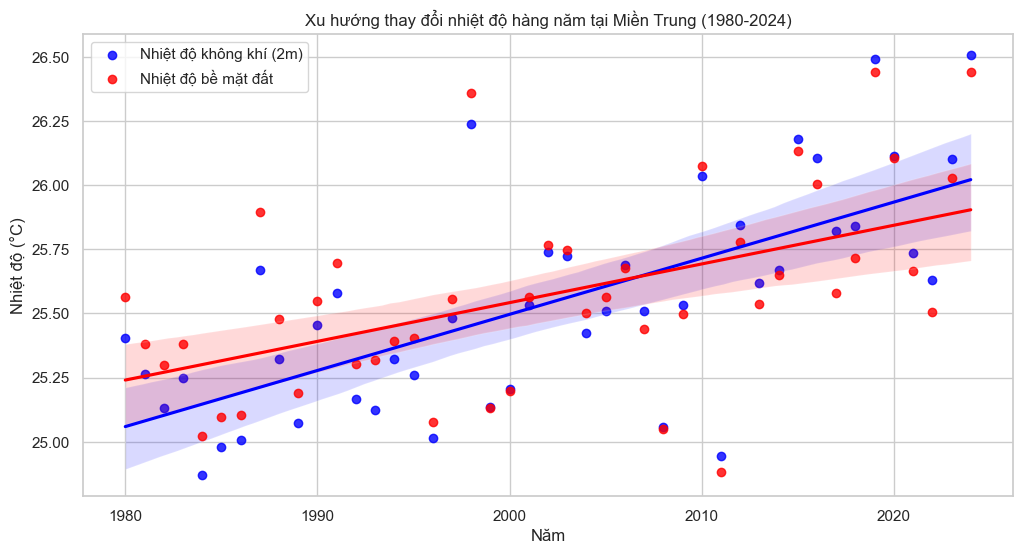
\includegraphics[width=\textwidth]{images/3.1.1.png}
        \caption{Xu hướng hàng năm}
    \end{subfigure}
    \hfill
    \begin{subfigure}[b]{0.48\textwidth}
        \centering
        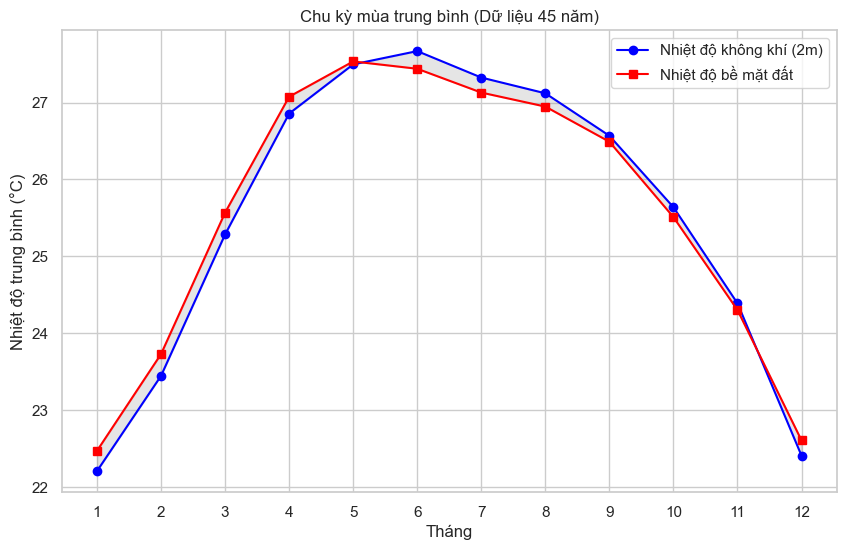
\includegraphics[width=\textwidth]{images/3.1.2.png}
        \caption{Chu kỳ mùa trung bình}
    \end{subfigure}
    \caption{Phân tích biến động nhiệt độ dài hạn và đặc trưng chu kỳ mùa tại miền Trung}
    \label{fig:temp_annual_seasonal}
\end{figure}
\FloatBarrier

\subsubsection{Ma trận dị thường nhiệt độ hàng tháng}
Ma trận tại \textbf{Hình \ref{fig:temp_anomaly_heatmap}} cung cấp cái nhìn chi tiết về độ lệch nhiệt độ so với trung bình nhiều năm trong giai đoạn 1980--2024.

\begin{itemize}
    \item \textbf{Đặc trưng khí hậu (RQ1):} Ma trận phản ánh sự chuyển dịch rõ rệt từ trạng thái "mát mẻ" ở hai thập kỷ đầu sang trạng thái "nóng liên tục" từ sau năm 2014. Dị thường dương không chỉ xuất hiện tập trung vào mùa hè mà còn lấn sang các tháng mùa đông, cho thấy xu hướng ấm hóa toàn phần đang diễn ra.
    \item \textbf{Tác nhân khắc nghiệt (RQ2):} Sự xuất hiện dày đặc của các mảng đỏ đậm trong thập kỷ gần đây minh chứng cho tác động của \textbf{biến đổi khí hậu toàn cầu} đã vượt qua khả năng điều tiết của hệ thống tự nhiên. Các năm El Niño cực đoan tạo ra những vệt nóng bất thường kéo dài, làm trầm trọng hóa tình trạng hạn hán và thiếu hụt nguồn nước.
\end{itemize}

\FloatBarrier
\begin{figure}[H]
    \centering
    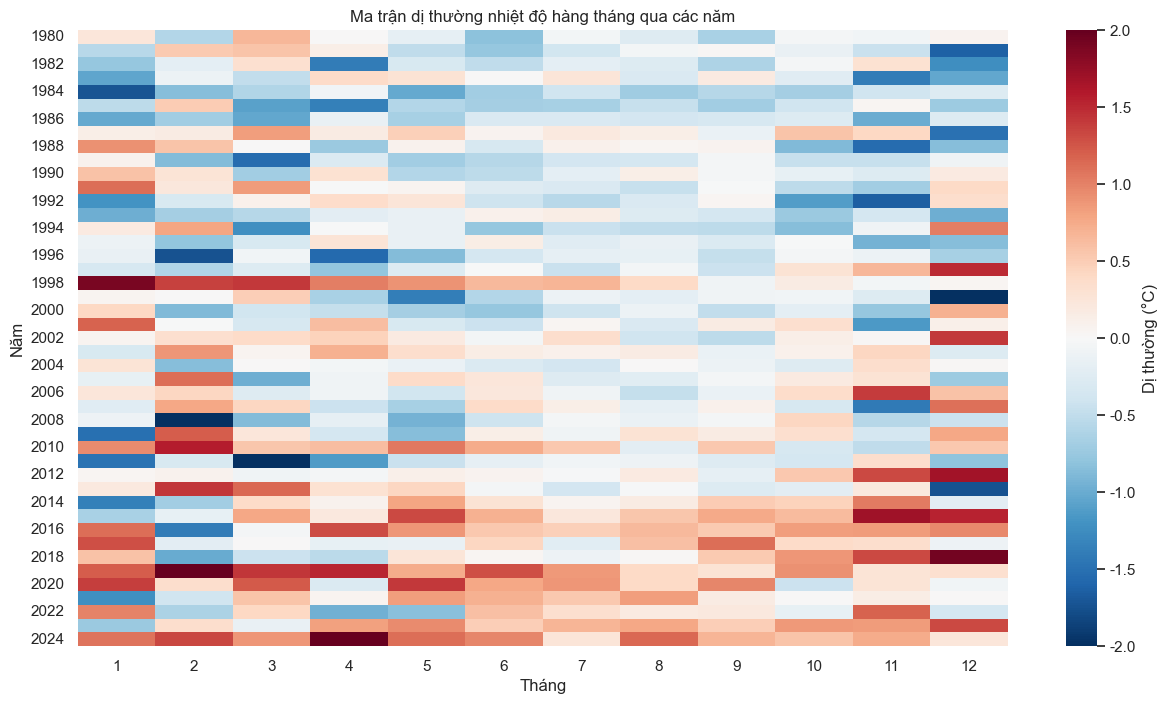
\includegraphics[width=0.7\textwidth]{images/3.1.3.png}
    \caption{Ma trận dị thường nhiệt độ hàng tháng tại miền Trung (1980--2024)}
    \label{fig:temp_anomaly_heatmap}
\end{figure}
\FloatBarrier

\subsubsection{Tần suất các ngày nắng nóng cực đoan}
Số lượng ngày nắng nóng (T\_trung bình $>32^\circ$C) tại \textbf{Hình \ref{fig:temp_extreme_dtr}(a)} cho thấy mức độ khốc liệt ngày càng gia tăng.

\begin{itemize}
    \item \textbf{Đặc trưng khí hậu (RQ1):} Tần suất nắng nóng cực đoan gia tăng đột biến, chuyển dịch từ mức dưới 10 ngày/năm trong quá khứ lên ngưỡng 20--35 ngày hiện nay. Đặc trưng này xác lập một "trạng thái bình thường mới" cho miền Trung, nơi các đợt nóng gay gắt xuất hiện với mật độ dày đặc hơn.
    \item \textbf{Tác nhân khắc nghiệt (RQ2):} Kỷ lục hơn 35 ngày vào năm 2024 phản ánh tác động cộng hưởng giữa biến đổi khí hậu và \textbf{vùng áp thấp nóng phía Tây} bị dãy Trường Sơn khuếch đại cường độ. Tác nhân này kết hợp với địa hình hẹp tạo ra các "bẫy nhiệt" kéo dài, trực tiếp đe dọa sức khỏe cộng đồng và an ninh năng lượng.
\end{itemize}

\subsubsection{Biến động biên độ nhiệt ngày (DTR)}
Chênh lệch nhiệt độ ngày đêm tại \textbf{Hình \ref{fig:temp_extreme_dtr}(b)} thể hiện xu hướng sụt giảm biên độ dao động nhiệt theo thời gian.

\begin{itemize}
    \item \textbf{Đặc trưng khí hậu (RQ1):} Xu hướng giảm DTR khẳng định nhiệt độ ban đêm tại miền Trung đang tăng nhanh hơn nhiệt độ ban ngày. Đặc trưng này làm mất đi tính ổn định nhiệt truyền thống, khiến chu kỳ nhiệt ngày đêm trở nên lệch lạc và khó thích nghi hơn cho sinh vật.
    \item \textbf{Tác nhân khắc nghiệt (RQ2):} Tác nhân gây giảm DTR chủ yếu là sự gia tăng \textbf{độ ẩm và mây đêm} từ Biển Đông, kết hợp hiệu ứng nhà kính cục bộ giữ nhiệt sát mặt đất. Điều này tạo ra sự khắc nghiệt "âm thầm" khi con người và cây trồng không có giai đoạn "nghỉ nhiệt" vào ban đêm trong các đợt nắng nóng.
\end{itemize}

\FloatBarrier
\begin{figure}[H]
    \centering
    \begin{subfigure}[b]{0.48\textwidth}
        \centering
        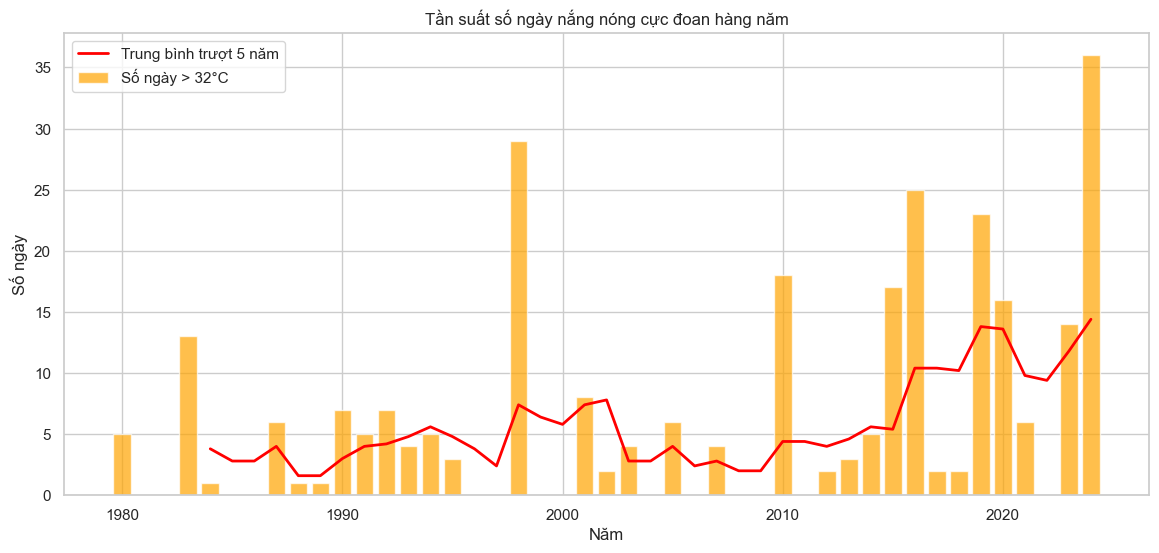
\includegraphics[width=\textwidth]{images/3.1.4.png}
        \caption{Tần suất ngày nắng nóng}
    \end{subfigure}
    \hfill
    \begin{subfigure}[b]{0.48\textwidth}
        \centering
        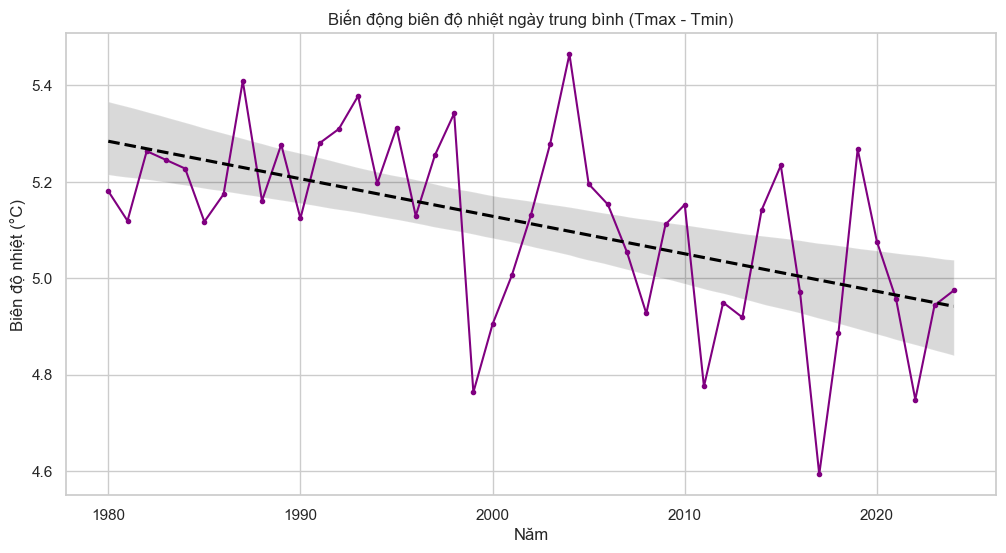
\includegraphics[width=\textwidth]{images/3.1.5.png}
        \caption{Biến động chỉ số DTR}
    \end{subfigure}
    \caption{Phân tích tần suất cực trị nhiệt độ và động lực biên độ nhiệt ngày đêm}
    \label{fig:temp_extreme_dtr}
\end{figure}
\FloatBarrier

\subsubsection{Sự dịch chuyển phân phối nhiệt độ qua các thập kỷ}
Sử dụng biểu đồ hộp tại \textbf{Hình \ref{fig:temp_dist_scatter}(a)} để quan sát sự thay đổi cấu trúc nhiệt độ qua 5 thập kỷ nghiên cứu.

\begin{itemize}
    \item \textbf{Đặc trưng khí hậu (RQ1):} Toàn bộ phân phối nhiệt độ dịch chuyển tịnh tiến lên phía nóng, với giá trị trung vị thập niên 2020 nay đã tiệm cận mức cực đại của thập niên 1980. Đây là minh chứng thống kê vững chắc cho việc miền Trung đang nóng lên một cách toàn diện và đồng nhất.
    \item \textbf{Tác nhân khắc nghiệt (RQ2):} Việc mở rộng giới hạn trên của các râu boxplot chứng minh các \textbf{hệ thống thời tiết nhiệt đới} đang tạo ra các ngưỡng nhiệt vượt ra ngoài các kịch bản lịch sử. Tác nhân cực đoan này buộc khu vực phải đối mặt với các sự kiện nhiệt độ "ngoại lai" xuất hiện với tần suất cao hơn.
\end{itemize}

\subsubsection{Tương quan vật lý giữa bề mặt đất và khí quyển}
Mối liên kết hữu cơ giữa đất và không khí tại \textbf{Hình \ref{fig:temp_dist_scatter}(b)} khẳng định vai trò nguồn nhiệt của mặt đệm.

\begin{itemize}
    \item \textbf{Đặc trưng khí hậu (RQ1):} Tương quan thuận cực mạnh ($r \approx 1$) duy trì qua các tháng, khẳng định bề mặt đất miền Trung là nguồn sưởi ấm chính cho khí quyển. Trong mùa đông, đất giữ nhiệt tốt hơn nên luôn ấm hơn không khí, tạo ra một đệm nhiệt ổn định cho lớp biên khí quyển.
    \item \textbf{Tác nhân khắc nghiệt (RQ2):} Sự đảo chiều tương quan vào mùa hè (không khí nóng hơn đất) là minh chứng cho tác động của \textbf{gió Lào}. Luồng gió này nung nóng khí quyển một cách cưỡng bức, phá vỡ thế cân bằng nhiệt tự nhiên và gây ra các đợt nóng khô khốc liệt ảnh hưởng đến sản xuất nông nghiệp.
\end{itemize}

\FloatBarrier
\begin{figure}[H]
    \centering
    \begin{subfigure}[b]{0.48\textwidth}
        \centering
        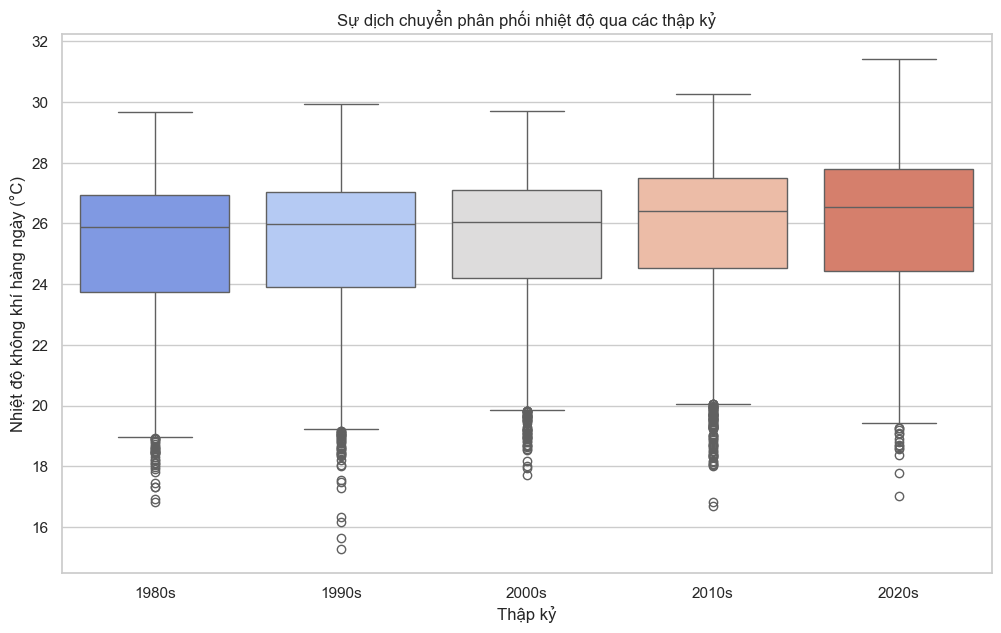
\includegraphics[width=\textwidth]{images/3.1.6.png}
        \caption{Phân phối qua các thập kỷ}
    \end{subfigure}
    \hfill
    \begin{subfigure}[b]{0.48\textwidth}
        \centering
        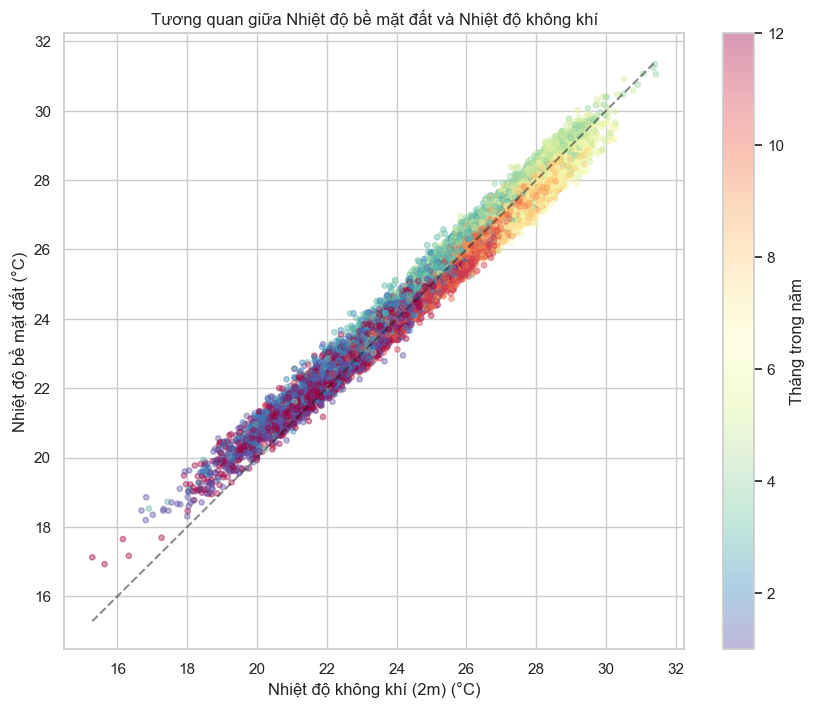
\includegraphics[width=\textwidth]{images/3.1.7.png}
        \caption{Tương quan Đất - Không khí}
    \end{subfigure}
    \caption{Phân tích dịch chuyển xác suất nhiệt độ và tương tác vật lý bề mặt đệm}
    \label{fig:temp_dist_scatter}
\end{figure}
\FloatBarrier

\subsection{Nhiệt độ đất}

\subsubsection{Sự lan truyền sóng nhiệt theo độ sâu đất \& Dấu hiệu nóng lên}
Sự xâm nhập nhiệt vào địa tầng miền Trung qua các thời kỳ được trực quan hóa tại \textbf{Hình \ref{fig:soil_propagation}}.

\begin{itemize}
    \item \textbf{Đặc trưng khí hậu (RQ1):} Nhiệt độ đất tuân theo quy luật trễ pha rõ rệt, khi đỉnh nhiệt ở độ sâu 289cm chậm hơn tầng mặt tới 3 tháng. Thổ nhưỡng khu vực đóng vai trò như một bộ lưu trữ nhiệt lượng, điều hòa các tác động tức thời từ khí quyển xuống sâu trong lòng đất.
    \item \textbf{Tác nhân khắc nghiệt (RQ2):} Việc nóng lên sâu 3m dưới lòng đất trong thập kỷ 2020 chứng minh \textbf{áp lực nhiệt bền vững} đã tích lũy trong địa tầng. Tác nhân này đe dọa sự ổn định của mực nước ngầm và làm thay đổi môi trường sống của hệ sinh vật đất vốn nhạy cảm với nhiệt độ.
\end{itemize}

\FloatBarrier
\begin{figure}[H]
    \centering
    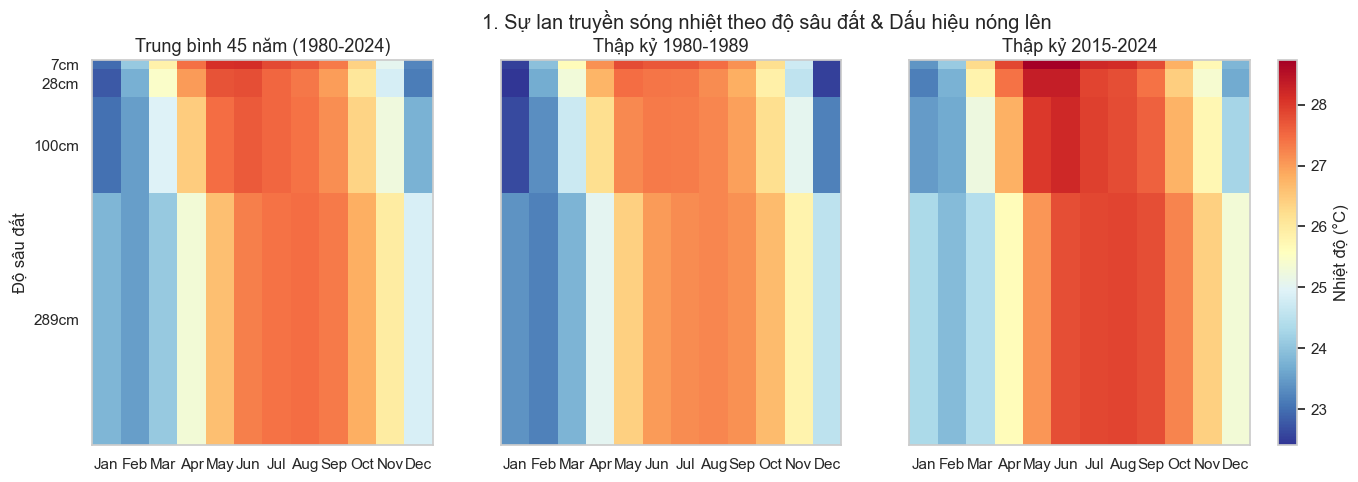
\includegraphics[width=0.7\textwidth]{images/3.2.1.png}
    \caption{Mặt cắt sự lan truyền sóng nhiệt theo độ sâu đất qua các thập kỷ}
    \label{fig:soil_propagation}
\end{figure}
\FloatBarrier

\subsubsection{Chu kỳ mùa nhiệt độ đất: Độ trễ pha và suy giảm biên độ}
Biến động nhiệt độ đất theo tháng tại \textbf{Hình \ref{fig:soil_cycle_trend}(a)} mô tả rõ sự suy giảm biên độ dao động nhiệt khi xuống sâu.

\begin{itemize}
    \item \textbf{Đặc trưng khí hậu (RQ1):} Biên độ dao động nhiệt giảm dần từ 5.3$^\circ$C xuống 4.0$^\circ$C ở tầng sâu nhất. Hiện tượng nghịch đảo nhiệt vào mùa đông (đất sâu ấm hơn bề mặt) là đặc trưng điều hòa nhiệt độ cốt lõi của thổ nhưỡng khu vực miền Trung.
    \item \textbf{Tác nhân khắc nghiệt (RQ2):} Sự chậm trễ của tầng 289cm khiến lòng đất vẫn duy trì mức nhiệt cao nhất của mùa hè đúng vào thời điểm bắt đầu mùa mưa bão tháng 10. Tác nhân tích nhiệt này tạo ra một môi trường nhiệt-ẩm phức tạp, ảnh hưởng đến các quá trình sinh hóa trong đất ngay khi bão lũ đổ bộ.
\end{itemize}

\subsubsection{Xu hướng nóng lên dài hạn tại các tầng đất}
Tốc độ tăng nhiệt năm tại \textbf{Hình \ref{fig:soil_cycle_trend}(b)} cho thấy sự biến đổi đồng nhất ở mọi tầng đất nghiên cứu.

\begin{itemize}
    \item \textbf{Đặc trưng khí hậu (RQ1):} Tốc độ nóng lên đạt trung bình +0.18$^\circ$C/thập kỷ tại mọi độ sâu, khẳng định biến đổi khí hậu đã trở thành xu hướng thay đổi cấu trúc nhiệt địa chất ổn định. Đặc trưng nóng lên toàn phần này chứng tỏ miền Trung đang chịu tác động sâu sắc từ khí quyển đến địa tầng.
    \item \textbf{Tác nhân khắc nghiệt (RQ2):} Tốc độ tăng nhanh nhất tại tầng mặt phản ánh tác động trực tiếp của các đợt \textbf{nắng nóng do gió Lào} ngày càng gay gắt. Tác nhân này đang dần nung nóng lớp đất canh tác nông nghiệp, làm gia tăng tốc độ bốc hơi ẩm từ lòng đất.
\end{itemize}

\FloatBarrier
\begin{figure}[H]
    \centering
    \begin{subfigure}[b]{0.48\textwidth}
        \centering
        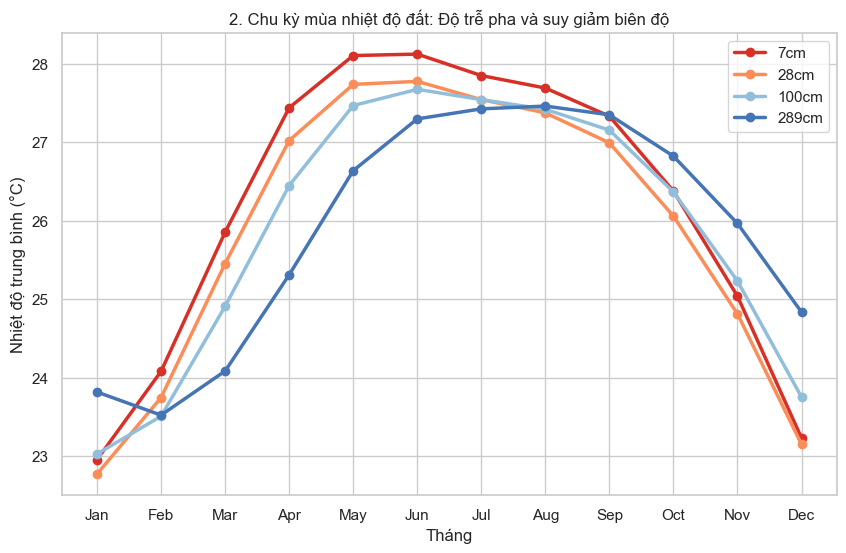
\includegraphics[width=\textwidth]{images/3.2.2.png}
        \caption{Chu kỳ mùa nhiệt độ đất}
    \end{subfigure}
    \hfill
    \begin{subfigure}[b]{0.48\textwidth}
        \centering
        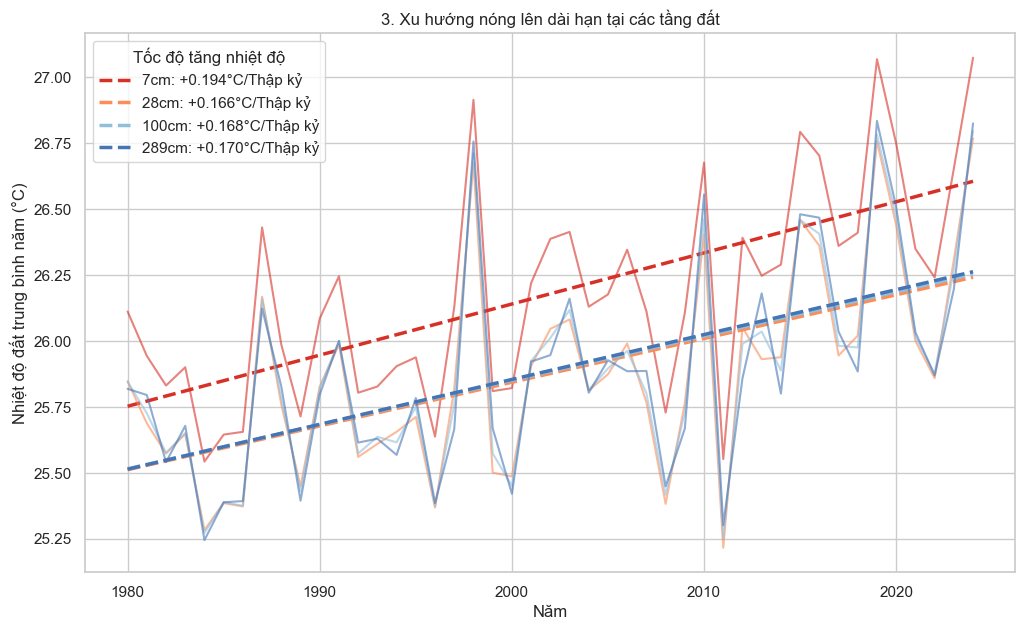
\includegraphics[width=\textwidth]{images/3.2.3.png}
        \caption{Xu hướng nóng lên dài hạn}
    \end{subfigure}
    \caption{Phân tích đặc trưng chu kỳ mùa và xu hướng biến đổi nhiệt độ địa chất}
    \label{fig:soil_cycle_trend}
\end{figure}
\FloatBarrier

\subsubsection{Ma trận dị thường nhiệt độ đất: Sự thẩm thấu của các năm cực đoan}
Ma trận tại \textbf{Hình \ref{fig:soil_anomaly_heatmap}} cung cấp cái nhìn chi tiết về cách các xung nhiệt bề mặt ngấm sâu xuống lòng đất qua 45 năm.

\begin{itemize}
    \item \textbf{Đặc trưng khí hậu (RQ1):} Đất miền Trung đóng vai trò như một "bộ nhớ khí hậu" lưu giữ các dị thường nhiệt bền vững hơn khí quyển. Các dị thường nóng xuất hiện ngắt quãng ở bề mặt thường được đất tầng sâu kết nối lại thành những mảng nóng liên tục kéo dài nhiều tháng.
    \item \textbf{Tác nhân khắc nghiệt (RQ2):} Sự biến mất hoàn toàn của dị thường âm (lạnh) sau năm 2014 ở các tầng sâu cho thấy \textbf{gió mùa Đông Bắc} không còn đủ sức trung hòa nhiệt lượng tích lũy. Tác nhân nóng lên từ biến đổi khí hậu đang chiếm ưu thế tuyệt đối, làm thay đổi nền nhiệt địa chất khu vực một cách tiêu cực.
\end{itemize}

\FloatBarrier
\begin{figure}[H]
    \centering
    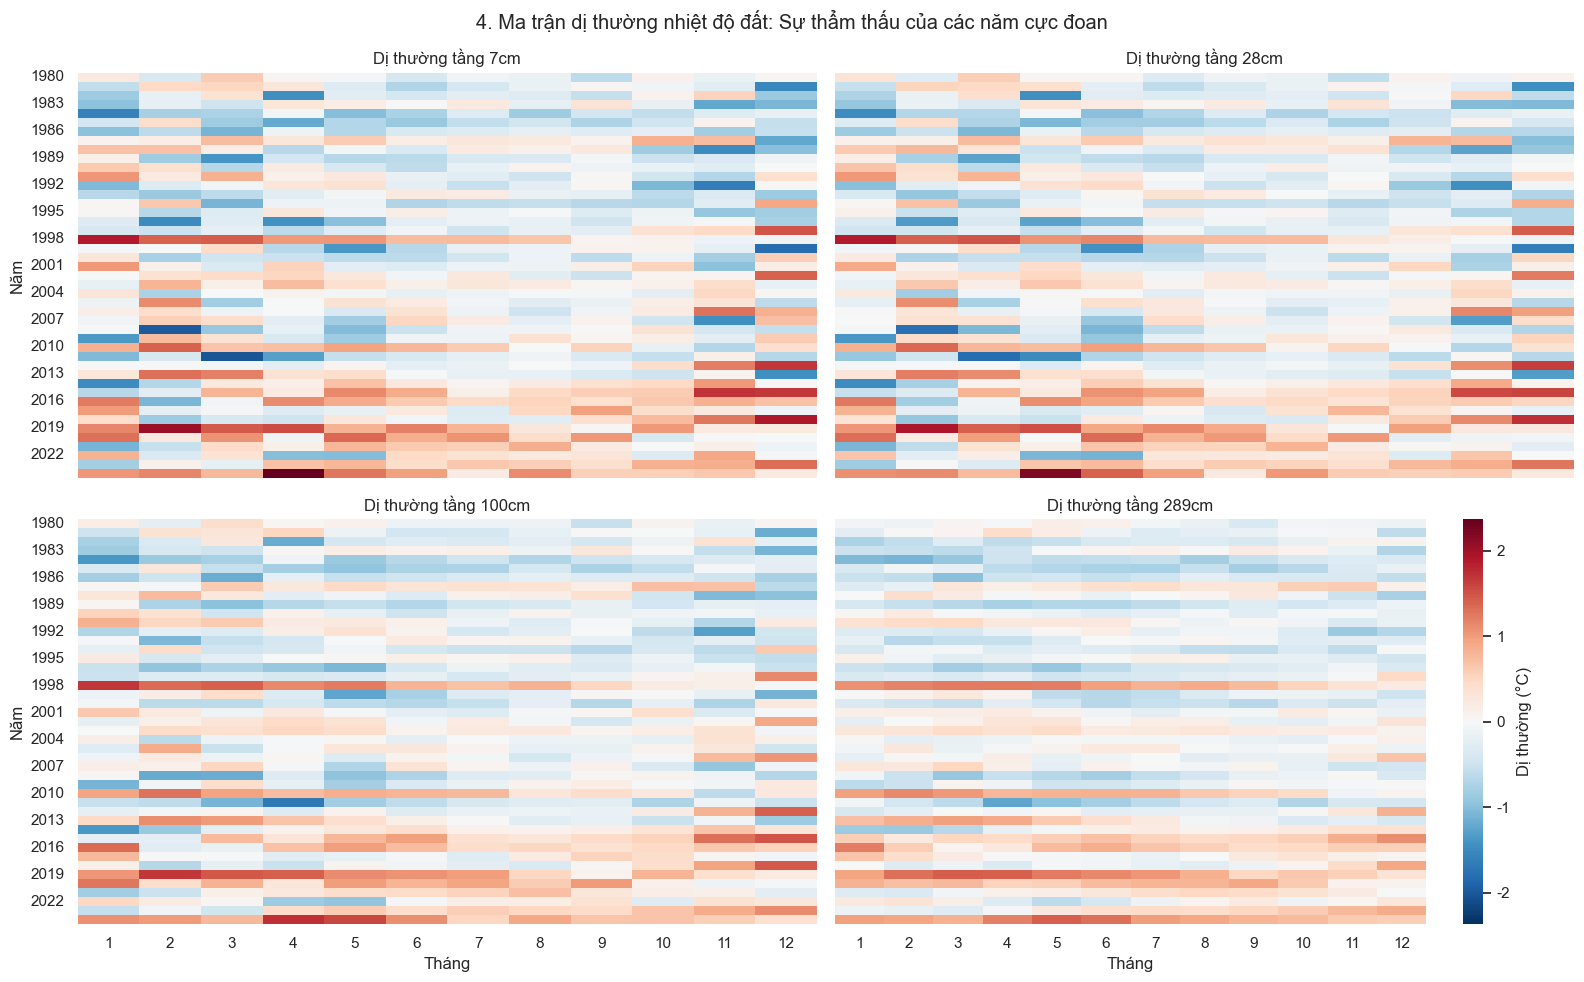
\includegraphics[width=0.7\textwidth]{images/3.2.4.png}
    \caption{Ma trận dị thường nhiệt độ đất tại 4 tầng sâu (1980--2024)}
    \label{fig:soil_anomaly_heatmap}
\end{figure}
\FloatBarrier

\subsubsection{Lượng hóa Độ trễ pha nhiệt (Thermal Lag) theo Độ sâu}
Mô hình hồi quy tại \textbf{Hình \ref{fig:soil_lag_correlation}(a)} xác lập đặc tính dẫn nhiệt định lượng của thổ nhưỡng miền Trung.

\begin{itemize}
    \item \textbf{Đặc trưng khí hậu (RQ1):} Quy luật truyền nhiệt được xác lập với tốc độ trễ trung bình \textbf{+1.1 tháng/mét sâu} với độ tin cậy $R^2=0.91$. Đây là thông số đặc trưng hệ thống mô tả khả năng trì hoãn và truyền dẫn năng lượng của cấu trúc địa chất địa phương.
    \item \textbf{Tác nhân khắc nghiệt (RQ2):} Quán tính nhiệt lớn khiến sự khắc nghiệt của nắng nóng mùa hè bị "kéo dài" thời gian ảnh hưởng xuống lòng đất thêm nhiều tháng. Tác nhân này tạo ra áp lực nhiệt tiềm tàng, làm suy kiệt độ ẩm rễ cây ngay cả khi không khí bề mặt đã bắt đầu mát mẻ.
\end{itemize}

\subsubsection{Tương quan và Cross-Correlation giữa các tầng đất}
Phân tích tương quan chéo tại \textbf{Hình \ref{fig:soil_lag_correlation}(b)} khẳng định sự liên kết động lực chặt chẽ giữa các tầng đất.

\begin{itemize}
    \item \textbf{Đặc trưng khí hậu (RQ1):} Hệ số tương quan chéo đạt đỉnh ($r=0.91$) chính xác tại \textbf{ngày thứ 33} cho độ sâu gần 3m. Điều này xác lập đặc trưng hệ thống về thời gian phản ứng đồng bộ của lòng đất miền Trung trước các biến động nhiệt bề mặt.
    \item \textbf{Tác nhân khắc nghiệt (RQ2):} Độ trễ 33 ngày khẳng định các tác nhân gây nóng bề mặt có sức ảnh hưởng xuyên suốt và bền bỉ. Một đợt nắng nóng kỷ lục sẽ mất trung bình 1 tháng để đạt đỉnh tác động ở tầng nước ngầm, duy trì trạng thái khắc nghiệt địa chất kéo dài.
\end{itemize}

\FloatBarrier
\begin{figure}[H]
    \centering
    \begin{subfigure}[b]{0.48\textwidth}
        \centering
        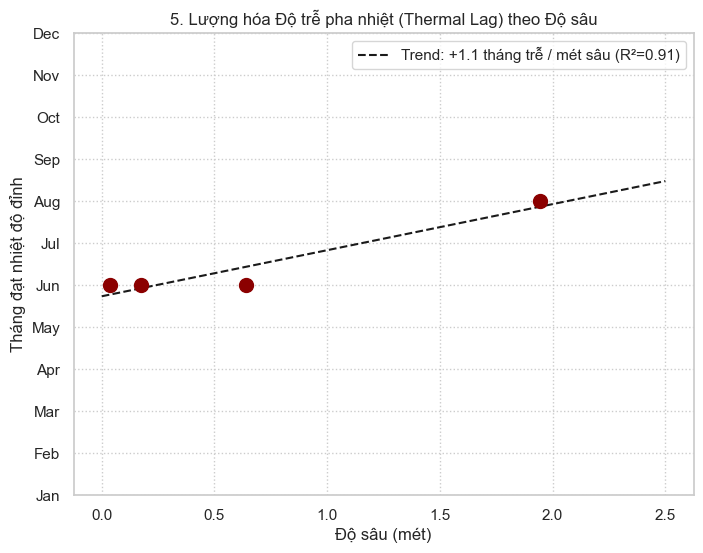
\includegraphics[width=\textwidth]{images/3.2.5.png}
        \caption{Lượng hóa độ trễ pha}
    \end{subfigure}
    \hfill
    \begin{subfigure}[b]{0.48\textwidth}
        \centering
        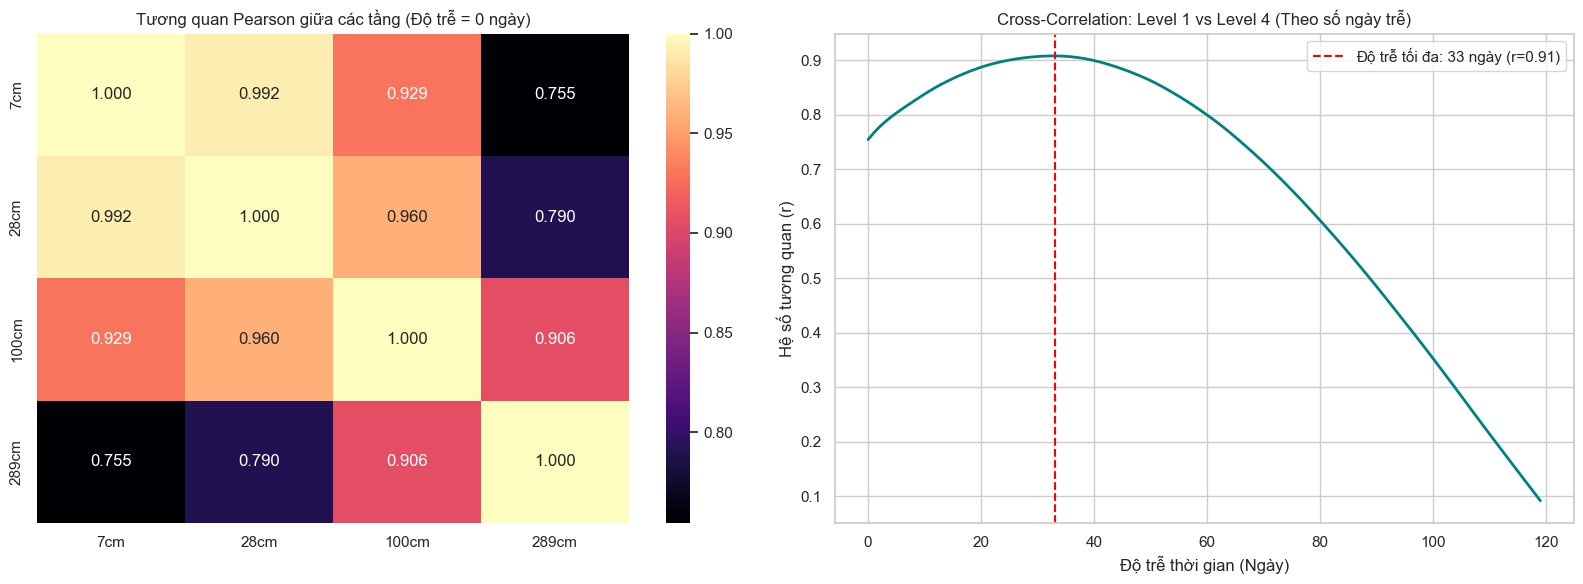
\includegraphics[width=\textwidth]{images/3.2.6.png}
        \caption{Phân tích Cross-Correlation}
    \end{subfigure}
    \caption{Định lượng đặc tính dẫn nhiệt và thời gian phản ứng của hệ thống đất}
    \label{fig:soil_lag_correlation}
\end{figure}
\FloatBarrier

\subsubsection{So sánh tương tác: Nhiệt độ bề mặt đất (Level 1) vs Nhiệt độ không khí}
Chênh lệch nhiệt lượng tại lớp biên tiếp giáp được thể hiện rõ qua chuỗi số liệu tại \textbf{Hình \ref{fig:soil_air_comp}}.

\begin{itemize}
    \item \textbf{Đặc trưng khí hậu (RQ1):} Bề mặt đất miền Trung luôn nóng hơn không khí khoảng 0.5--0.8$^\circ$C quanh năm, đóng vai trò "lò nhiệt" sưởi ấm khí quyển. Đặc trưng này biến mặt đất thành nguồn năng lượng chính chi phối toàn bộ chu trình nhiệt-ẩm của khu vực.
    \item \textbf{Tác nhân khắc nghiệt (RQ2):} Sự chênh lệch nhiệt độ này đạt đỉnh vào các năm nắng nóng kỷ lục, thúc đẩy quá trình đối lưu mạnh gây dông lốc cực đoan. Tác nhân chênh lệch nhiệt lớn cũng làm trầm trọng hóa quá trình bốc hơi ẩm, khiến hạn hán khốc liệt hơn tại miền Trung.
\end{itemize}

\FloatBarrier
\begin{figure}[H]
    \centering
    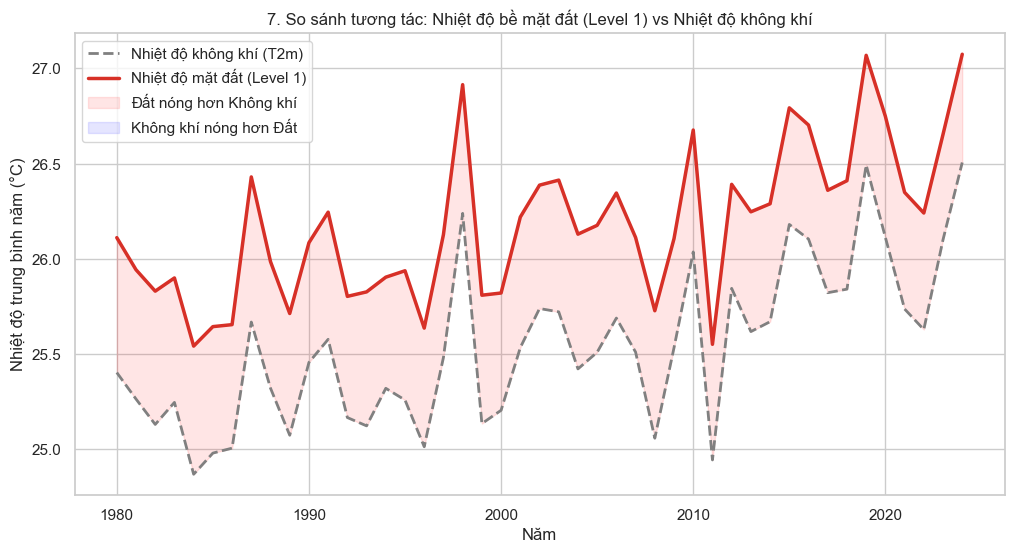
\includegraphics[width=0.7\textwidth]{images/3.2.7.png}
    \caption{So sánh biến động nhiệt độ bề mặt đất (Level 1) và nhiệt độ không khí (2m)}
    \label{fig:soil_air_comp}
\end{figure}
\FloatBarrier

\subsection{Điểm sương và độ ẩm}

\subsubsection{Khí hậu học theo mùa: Nhiệt độ điểm sương vs Nhiệt độ không khí}
Đặc trưng nhiệt-ẩm tại \textbf{Hình \ref{fig:dewpoint_overview}(a)} cho thấy độ ẩm miền Trung luôn duy trì ở nền cao ổn định.

\begin{itemize}
    \item \textbf{Đặc trưng khí hậu (RQ1):} Nhiệt độ điểm sương ($T_d$) bám sát nhiệt độ không khí quanh năm, đạt đáy tháng 1 (~17$^\circ$C) và đỉnh tháng 6 (~24$^\circ$C). Chênh lệch điểm sương thấp cho thấy không khí khu vực luôn ở trạng thái gần bão hòa hơi nước, xác lập đặc tính nóng ẩm điển hình.
    \item \textbf{Tác nhân khắc nghiệt (RQ2):} Vào mùa hè, tác nhân \textbf{Biển Đông} bơm ẩm liên tục khiến $T_d$ duy trì mức rất cao ngay cả khi nhiệt độ không khí cực đại. Tác nhân này làm tăng chỉ số nhiệt (Heat Index), biến các đợt nắng nóng miền Trung trở nên "oi bức cực đoan", gây áp lực lớn lên cơ thể người.
\end{itemize}

\subsubsection{Chu kỳ mùa và xu hướng của chênh lệch điểm sương (DPD)}
Dựa trên \textbf{Hình \ref{fig:dewpoint_overview}(b)}, DPD thấp nhất vào tháng 9 (~3.0$^\circ$C) cho thấy trạng thái gần bão hòa hơi nước nhất vào cuối năm.

\begin{itemize}
    \item \textbf{Đặc trưng khí hậu (RQ1):} Đặc trưng không khí miền Trung gần đạt bão hòa hoàn toàn vào cao điểm mùa mưa bão, tạo điều kiện thuận lợi cho sự ngưng tụ mạnh. Xu hướng dài hạn ổn định cho thấy đặc tính khô/ẩm của khu vực không có sự dịch chuyển quá lớn về cấu trúc mùa.
    \item \textbf{Tác nhân khắc nghiệt (RQ2):} Khoảng cách DPD nới rộng tháng 2--3 do khối khí lục địa khô từ phía Bắc tràn về. Sự sụt giảm DPD mạnh từ tháng 5 là dấu ấn của nguồn ẩm dồi dào từ \textbf{Biển Đông} và dải hội tụ ITCZ bắt đầu chi phối hoàn toàn khí quyển khu vực.
\end{itemize}

\FloatBarrier
\begin{figure}[H]
    \centering
    \begin{subfigure}[b]{0.48\textwidth}
        \centering
        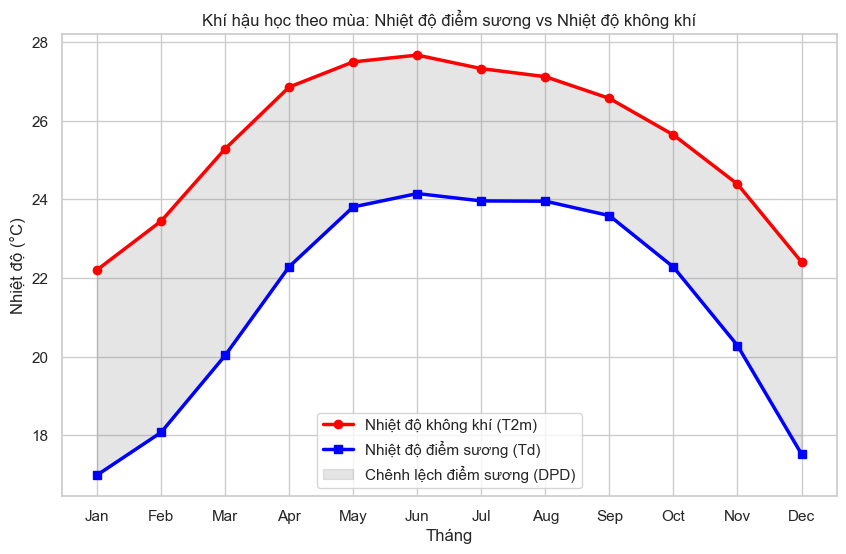
\includegraphics[width=\textwidth]{images/3.3.1.png}
        \caption{Chu kỳ mùa Td và T2m}
    \end{subfigure}
    \hfill
    \begin{subfigure}[b]{0.48\textwidth}
        \centering
        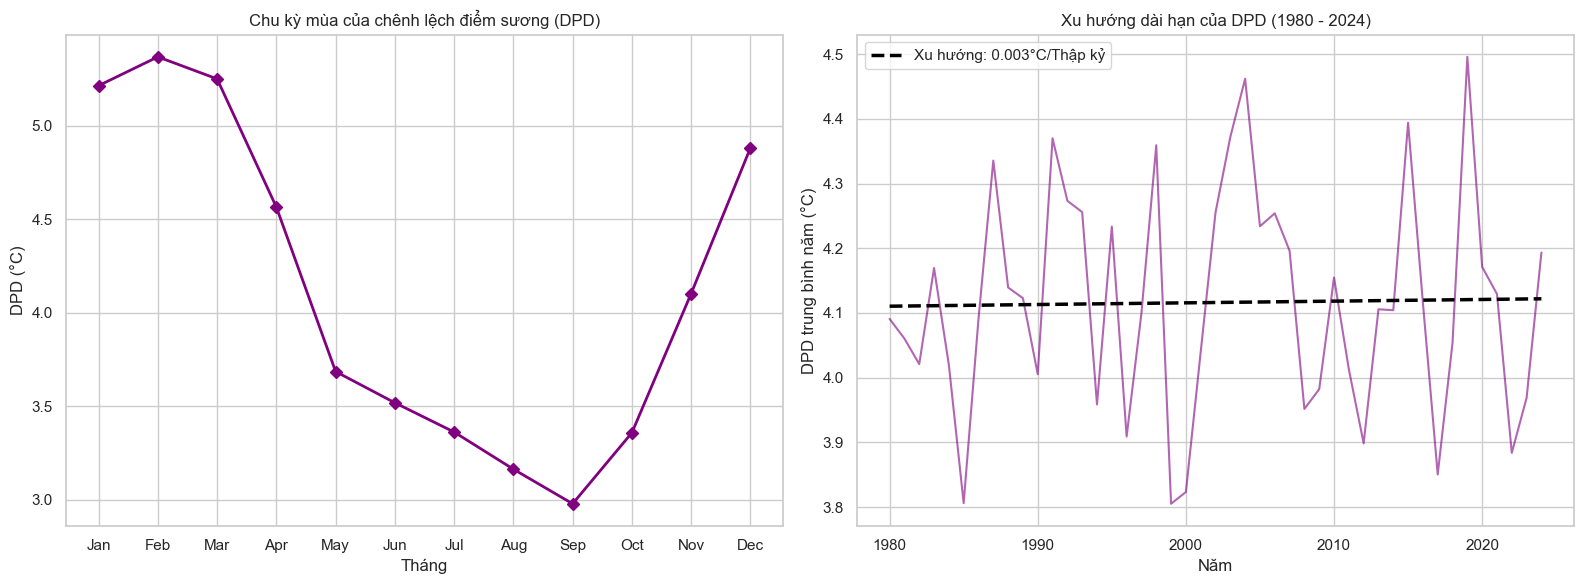
\includegraphics[width=\textwidth]{images/3.3.2.png}
        \caption{Chu kỳ và xu hướng DPD}
    \end{subfigure}
    \caption{Đặc trưng trạng thái ẩm và độ lệch nhiệt độ điểm sương khí quyển miền Trung}
    \label{fig:dewpoint_overview}
\end{figure}
\FloatBarrier

\subsubsection{Xu hướng dài hạn của Nhiệt độ điểm sương (so sánh với T2m)}
Xu hướng tăng hơi nước khí quyển được minh chứng rõ rệt tại \textbf{Hình \ref{fig:td_trend_anomaly}(a)}.

\begin{itemize}
    \item \textbf{Đặc trưng khí hậu (RQ1):} $T_d$ tăng với tốc độ +0.216$^\circ$C/thập kỷ, song hành cùng tốc độ nóng lên của nhiệt độ không khí. Điều này xác lập đặc trưng miền Trung đang trở nên "giàu ẩm" hơn trong bối cảnh ấm hóa toàn cầu, làm thay đổi cán cân nhiệt-ẩm khu vực.
    \item \textbf{Tác nhân khắc nghiệt (RQ2):} Việc tăng $T_d$ song hành với nhiệt độ làm gia tăng năng lượng tiềm tàng trong khí quyển. Tác nhân này khiến các sóng nhiệt không chỉ nóng hơn mà còn ẩm hơn, làm suy giảm khả năng thoát mồ hôi của con người, trực tiếp gia tăng rủi ro sốc nhiệt.
\end{itemize}

\subsubsection{Ma trận dị thường Nhiệt độ điểm sương}
Biến động độ ẩm lịch sử được trực quan hóa qua ma trận tại \textbf{Hình \ref{fig:td_trend_anomaly}(b)}.

\begin{itemize}
    \item \textbf{Đặc trưng khí hậu (RQ1):} Có sự chuyển dịch từ trạng thái khô hơn trung bình (màu nâu) sang trạng thái ẩm bất thường (xanh lục) sau mốc 2010. Dị thường dương (ẩm) ngày càng áp đảo dị thường âm, phản ánh đặc trưng biến đổi khí hậu đang làm giàu hơi nước khí quyển.
    \item \textbf{Tác nhân khắc nghiệt (RQ2):} Các năm dị thường dương mạnh gần đây trùng khớp với các đợt bão lũ kỷ lục tại miền Trung. Tác nhân hơi nước tăng cao bất thường là tiền đề cho các hiện tượng mưa cực đoan có cường suất lớn, vượt quá khả năng chống chịu của hạ tầng khu vực.
\end{itemize}

\FloatBarrier
\begin{figure}[H]
    \centering
    \begin{subfigure}[b]{0.48\textwidth}
        \centering
        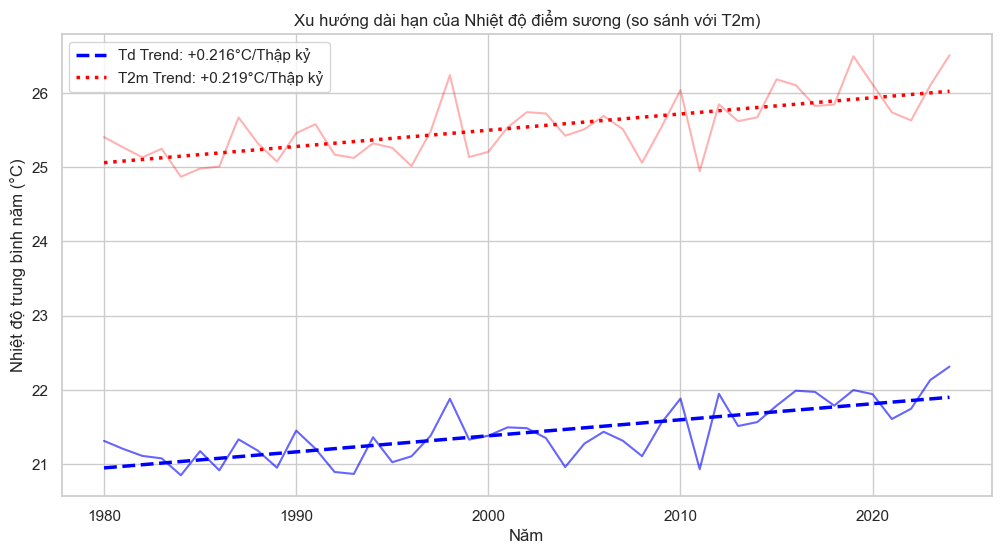
\includegraphics[width=\textwidth]{images/3.3.3.png}
        \caption{Xu hướng dài hạn Td}
    \end{subfigure}
    \hfill
    \begin{subfigure}[b]{0.48\textwidth}
        \centering
        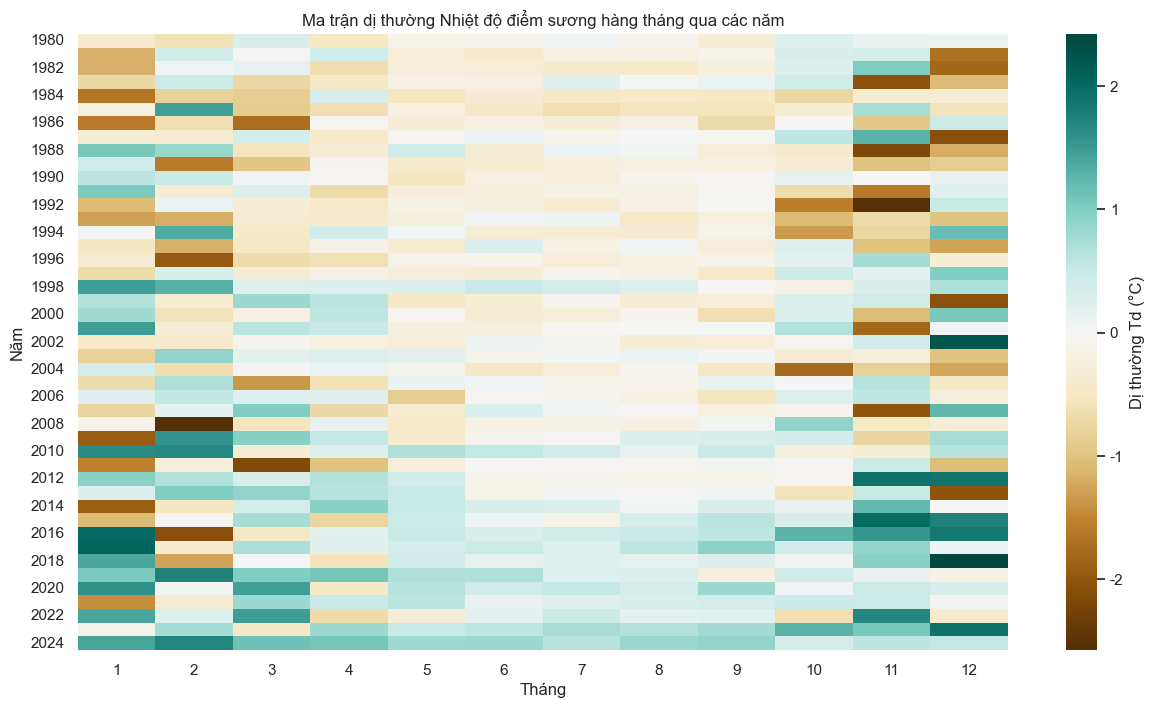
\includegraphics[width=\textwidth]{images/3.3.4.png}
        \caption{Ma trận dị thường Td}
    \end{subfigure}
    \caption{Phân tích xu hướng ấm hóa hơi nước và phân bổ dị thường điểm sương lịch sử}
    \label{fig:td_trend_anomaly}
\end{figure}
\FloatBarrier

\subsubsection{Tương quan Nhiệt độ điểm sương và Nhiệt độ không khí}
Biểu đồ phân tán tại \textbf{Hình \ref{fig:td_scatter_extreme}(a)} thể hiện giới hạn vật lý của hơi nước khí quyển miền Trung.

\begin{itemize}
    \item \textbf{Đặc trưng khí hậu (RQ1):} Các điểm dữ liệu bám sát đường bão hòa ở mọi dải nhiệt độ, khẳng định độ ẩm khu vực luôn duy trì ở mức cận bão hòa. Đặc trưng này cho thấy khí quyển miền Trung phản ứng cực kỳ nhạy bén với bất kỳ sự thay đổi nhiệt độ nào từ mặt đệm.
    \item \textbf{Tác nhân khắc nghiệt (RQ2):} Ở dải nhiệt độ cao mùa hè, $T_d$ duy trì cao là do tác nhân \textbf{Biển Đông} liên tục bơm ẩm vào đất liền. Sự kết hợp giữa nhiệt cao và ẩm lớn tạo ra môi trường cực đoan cho sinh vật, làm tăng cảm giác oi bức thực tế so với nhiệt độ dự báo.
\end{itemize}

\subsubsection{Tần suất số ngày độ ẩm cao cực đoan}
Số ngày bão hòa ẩm được trình bày cụ thể qua biểu đồ tại \textbf{Hình \ref{fig:td_scatter_extreme}(b)}.

\begin{itemize}
    \item \textbf{Đặc trưng khí hậu (RQ1):} Số ngày có độ ẩm trung bình $>85\%$ thường xuyên vượt mức 50 ngày/năm và duy trì nền cao qua chu kỳ trung bình trượt 5 năm. Đây là đặc trưng khí hậu "ướt" bền bỉ của dải đất ven biển miền Trung, ảnh hưởng trực tiếp đến hệ sinh thái và đời sống dân cư.
    \item \textbf{Tác nhân khắc nghiệt (RQ2):} Các đỉnh điểm ẩm cao cực đoan trùng khớp hoàn toàn các năm hoạt động mạnh của \textbf{bão và ITCZ}. Tác nhân hơi nước bão hòa duy trì nhiều ngày liên tục là nguyên nhân gây hư hỏng hạ tầng, nấm mốc nông sản và các dịch bệnh liên quan đến độ ẩm cao.
\end{itemize}

\FloatBarrier
\begin{figure}[H]
    \centering
    \begin{subfigure}[b]{0.48\textwidth}
        \centering
        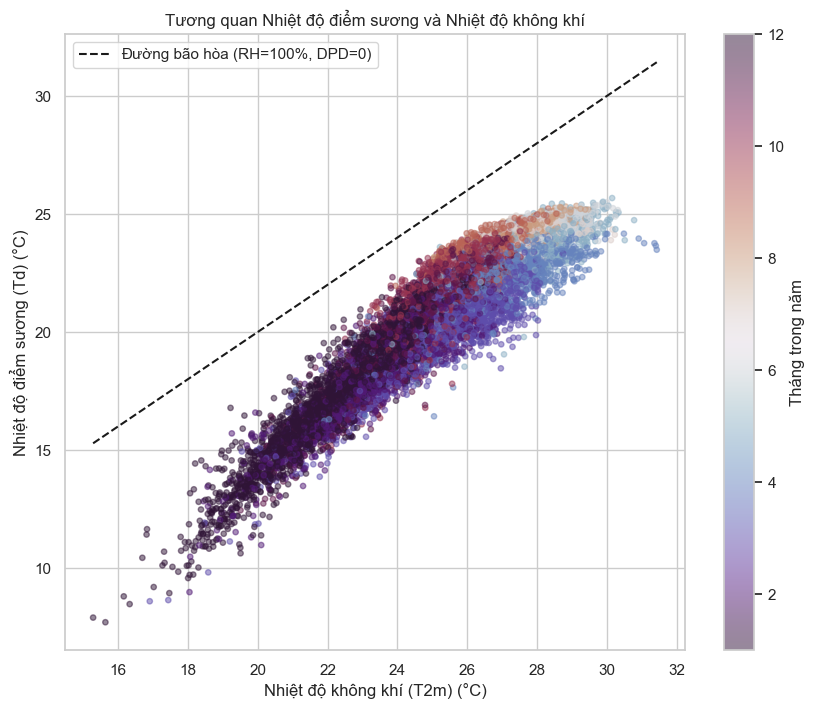
\includegraphics[width=\textwidth]{images/3.3.5.png}
        \caption{Tương quan Td vs T2m}
    \end{subfigure}
    \hfill
    \begin{subfigure}[b]{0.48\textwidth}
        \centering
        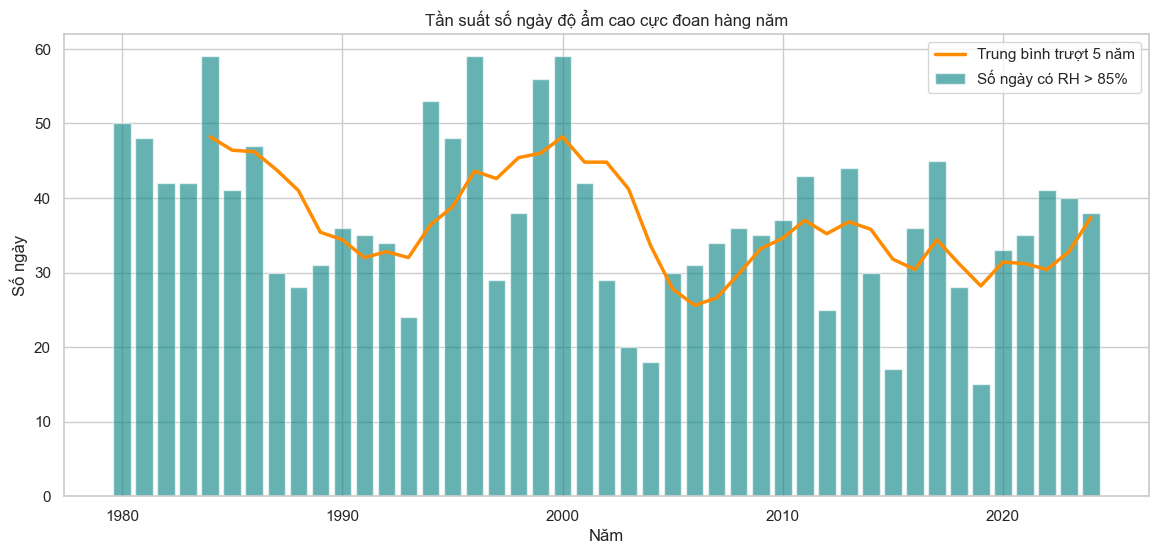
\includegraphics[width=\textwidth]{images/3.3.6.png}
        \caption{Số ngày RH $> 85\%$}
    \end{subfigure}
    \caption{Phân tích giới hạn chứa ẩm và tần suất trạng thái ẩm cực đoan khí quyển}
    \label{fig:td_scatter_extreme}
\end{figure}
\FloatBarrier

\subsubsection{Chu kỳ ngày đêm của Nhiệt độ điểm sương theo mùa}
Đặc trưng ngày đêm của độ ẩm tại \textbf{Hình \ref{fig:td_diurnal}} cho thấy $T_d$ có tính ổn định rất cao suốt 24 giờ.

\begin{itemize}
    \item \textbf{Đặc trưng khí hậu (RQ1):} $T_d$ có biên độ dao động ngày đêm cực nhỏ so với nhiệt độ không khí. Mùa Hè đạt mức $T_d$ cao nhất và ổn định nhất (~24$^\circ$C), trong khi mùa Đông thấp nhất (~17.5$^\circ$C) nhưng vẫn duy trì đường ngang thẳng tắp suốt chu kỳ ngày.
    \item \textbf{Tác nhân khắc nghiệt (RQ2):} Sự ổn định của $T_d$ cao vào ban đêm mùa hè ngăn cản quá trình giải nhiệt tự nhiên của khí quyển. Do tác nhân \textbf{khối khí biển} xâm nhập sâu, miền Trung không thể hạ nhiệt ban đêm, tạo trạng thái ngột ngạt xuyên suốt 24 giờ gây căng thẳng nhiệt cho hệ sinh vật.
\end{itemize}

\FloatBarrier
\begin{figure}[H]
    \centering
    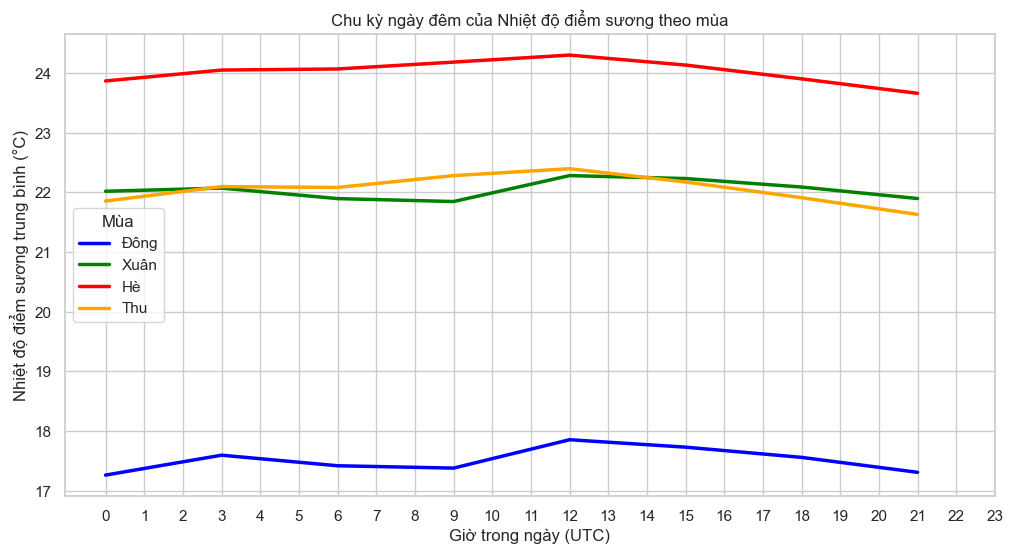
\includegraphics[width=0.7\textwidth]{images/3.3.7.png}
    \caption{Chu kỳ ngày đêm của Nhiệt độ điểm sương trung bình theo các mùa}
    \label{fig:td_diurnal}
\end{figure}
\FloatBarrier

\subsection{Lượng hơi nước và mây}

\subsubsection{Khí hậu học mùa: Hơi nước và Thành phần mây}
Động lực hơi nước và nước mây tại \textbf{Hình \ref{fig:vapor_cloud_overview}(a)} phản ánh quá trình tích ẩm nhiệt đới khu vực.

\begin{itemize}
    \item \textbf{Đặc trưng khí hậu (RQ1):} Tổng hơi nước cột (TCWV) đạt đỉnh tháng 6--8 (~55 kg/m$^2$), trong khi nước lỏng trong mây đạt đỉnh muộn hơn vào tháng 9--10. Đặc trưng này cho thấy một quá trình tích lũy ẩm dài ngày trước khi bùng nổ các hệ thống gây mưa dồn dập vào cuối năm.
    \item \textbf{Tác nhân khắc nghiệt (RQ2):} Sự hội tụ hơi nước tối đa tháng 9--10 trùng khớp hoàn toàn với cao điểm \textbf{mùa bão miền Trung}. Khối lượng hơi nước khổng lồ này bị cưỡng bức ngưng tụ bởi các động lực xoáy thuận, là tác nhân trực tiếp gây ra các trận mưa lũ có quy mô thảm họa.
\end{itemize}

\subsubsection{Chu kỳ mùa của tỷ lệ băng trong mây (Ice Fraction)}
Tỷ lệ pha băng khí quyển tại \textbf{Hình \ref{fig:vapor_cloud_overview}(b)} cho thấy cấu trúc vật lý của mây miền Trung theo mùa.

\begin{itemize}
    \item \textbf{Đặc trưng khí hậu (RQ1):} Tỷ lệ băng duy trì ở ngưỡng cao ($>0.3$) suốt mùa hè từ tháng 6 đến tháng 9. Đặc trưng này phản ánh bầu trời miền Trung mùa hè bị thống trị bởi các đám mây đối lưu phát triển mạnh lên các tầng cao lạnh của khí quyển.
    \item \textbf{Tác nhân khắc nghiệt (RQ2):} Tỷ lệ băng cao mùa hè minh chứng cho các \textbf{quá trình đối lưu sâu} cực mạnh do nung nóng mặt đệm kết hợp hiệu ứng phơn. Tác nhân này kích phát các hiện tượng giông sét, lốc xoáy và mưa đá đột ngột vùng giáp ranh Trường Sơn, gây thiệt hại lớn cho nông nghiệp.
\end{itemize}

\FloatBarrier
\begin{figure}[H]
    \centering
    \begin{subfigure}[b]{0.48\textwidth}
        \centering
        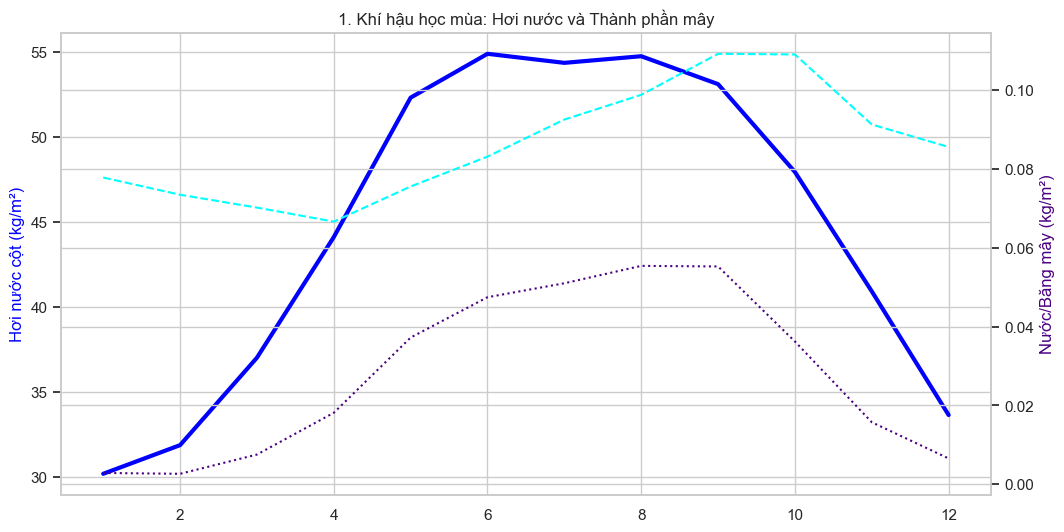
\includegraphics[width=\textwidth]{images/3.4.1.png}
        \caption{Chu kỳ mùa TCWV}
    \end{subfigure}
    \hfill
    \begin{subfigure}[b]{0.48\textwidth}
        \centering
        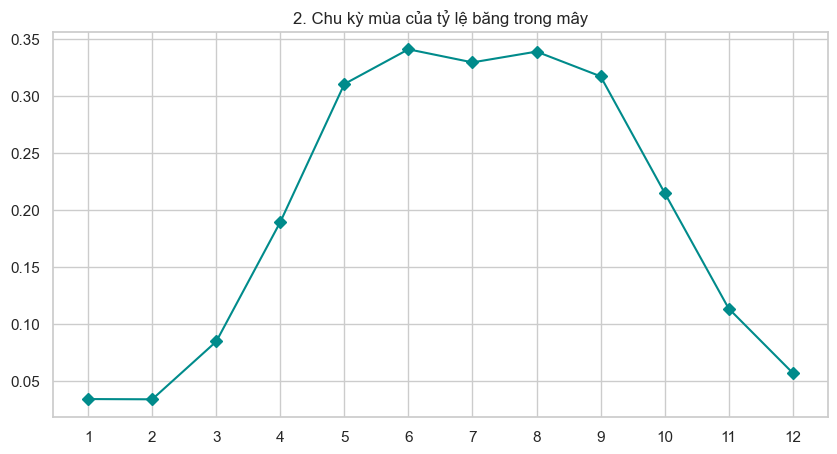
\includegraphics[width=\textwidth]{images/3.4.2.png}
        \caption{Chu kỳ tỷ lệ băng trong mây}
    \end{subfigure}
    \caption{Đặc trưng tích ẩm và pha ngưng tụ của hệ thống mây nhiệt đới miền Trung}
    \label{fig:vapor_cloud_overview}
\end{figure}
\FloatBarrier

\subsubsection{Xu hướng dài hạn của Tổng hơi nước cột (TCWV)}
Biến đổi dài hạn hơi nước tại \textbf{Hình \ref{fig:tcwv_trend_anomaly}(a)} đạt mức tăng +0.531 kg/m$^2$ mỗi thập kỷ.

\begin{itemize}
    \item \textbf{Đặc trưng khí hậu (RQ1):} Khí quyển miền Trung ngày càng trở nên "giàu năng lượng" hơn do chứa nhiều hơi nước tích hợp theo cột đứng. Đặc trưng ấm hóa hơi nước này tạo tiền đề cho sự gia tăng cường độ của tất cả các hệ thống thời tiết nhiệt đới hoạt động tại khu vực.
    \item \textbf{Tác nhân khắc nghiệt (RQ2):} Sự nóng lên của nước biển \textbf{Biển Đông} làm tăng cường bốc hơi, bơm thêm ẩm vào cột khí quyển. Tác nhân hơi nước dồi dào này đóng vai trò "nhiên liệu" làm bão nhiệt đới khi tiến vào ven bờ có xu hướng duy trì hoặc tăng cấp đột ngột, khó dự báo hơn.
\end{itemize}

\subsubsection{Ma trận dị thường Hơi nước cột}
Biến động dị thường ẩm lịch sử được trực quan hóa qua ma trận tại \textbf{Hình \ref{fig:tcwv_trend_anomaly}(b)}.

\begin{itemize}
    \item \textbf{Đặc trưng khí hậu (RQ1):} Ma trận phản ánh sự áp đảo của các tháng dư thừa ẩm (màu xanh) từ sau năm 2015 so với giai đoạn trước. Các giai đoạn khô hạn (màu đỏ) và ẩm ướt đan xen cực đoan, xác lập tính bất ổn định cao của năng lượng ẩm miền Trung.
    \item \textbf{Tác nhân khắc nghiệt (RQ2):} Sự thiếu hụt ẩm nghiêm trọng vào các năm \textbf{El Niño mạnh} (1998, 2010) là tác nhân trực tiếp gây ra hạn hán và xâm nhập mặn. Ngược lại, các vệt xanh đậm kéo dài là dấu ấn của các đợt mưa lũ kỷ lục tàn phá hạ tầng khu vực trong thập kỷ qua.
\end{itemize}

\FloatBarrier
\begin{figure}[H]
    \centering
    \begin{subfigure}[b]{0.48\textwidth}
        \centering
        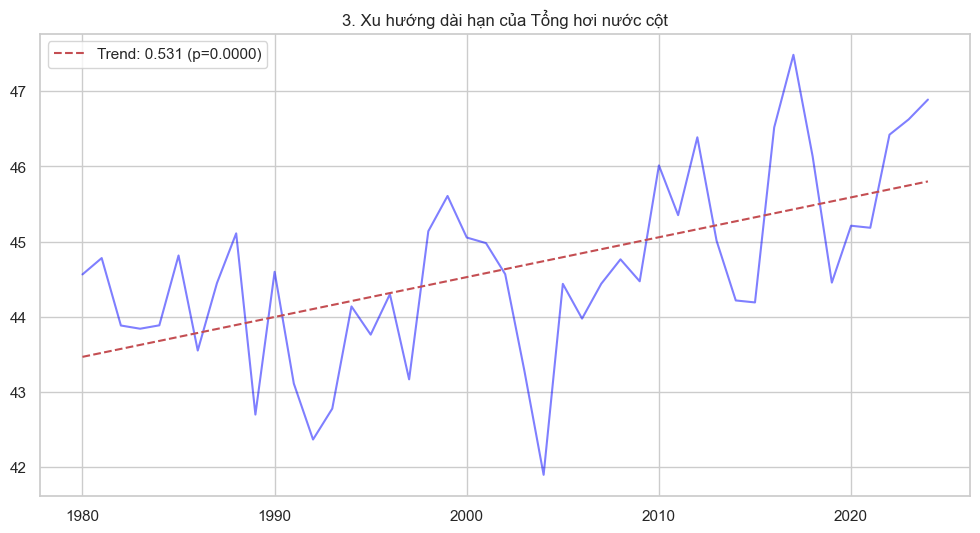
\includegraphics[width=\textwidth]{images/3.4.3.png}
        \caption{Xu hướng dài hạn TCWV}
    \end{subfigure}
    \hfill
    \begin{subfigure}[b]{0.48\textwidth}
        \centering
        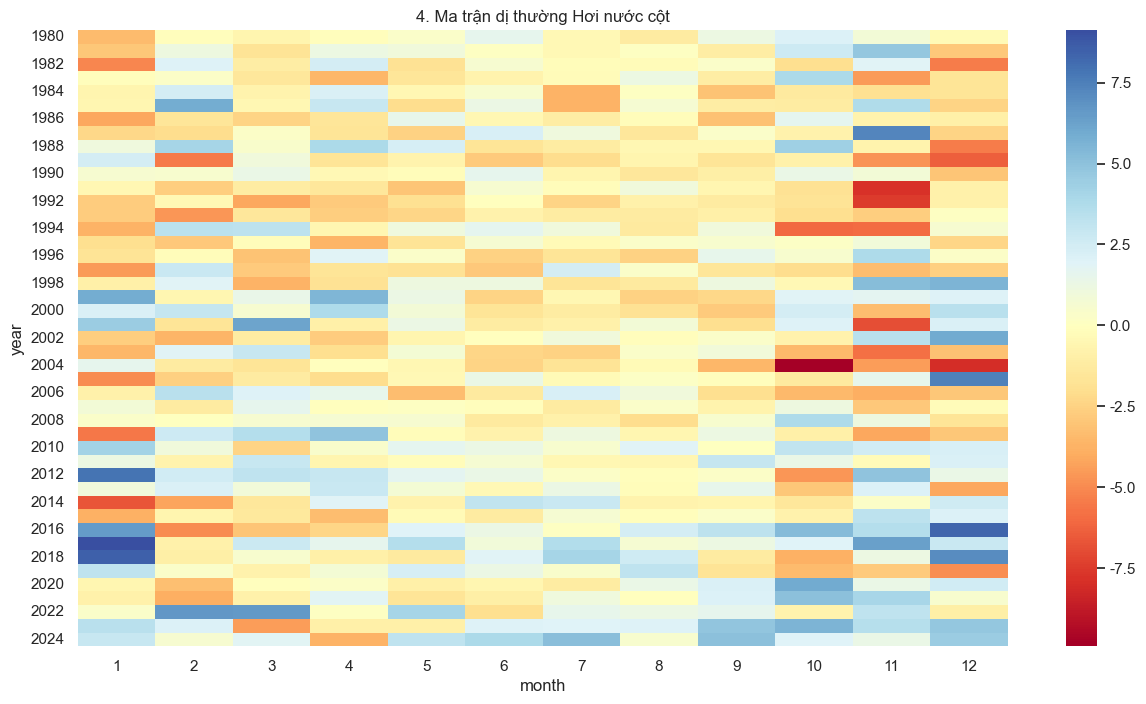
\includegraphics[width=\textwidth]{images/3.4.4.png}
        \caption{Ma trận dị thường TCWV}
    \end{subfigure}
    \caption{Phân tích xu hướng ấm hóa hơi nước cột và dị thường năng lượng ẩm khí quyển}
    \label{fig:tcwv_trend_anomaly}
\end{figure}
\FloatBarrier

\subsubsection{Phân chia pha mây theo thời gian}
Động lực các thành phần nước mây tại \textbf{Hình \ref{fig:cloud_phase_scatter}(a)} thể hiện tính chất đa dạng của mây khu vực.

\begin{itemize}
    \item \textbf{Đặc trưng khí hậu (RQ1):} Mây miền Trung chủ yếu tồn tại ở pha lỏng (CLW), các xung đỉnh pha băng (CIW) xuất hiện dồn dập vào mùa mưa bão. Đặc trưng này phản ánh một hệ thống mây nhiệt đới có cấu trúc thẳng đứng phát triển mạnh, đặc biệt vào nửa cuối năm.
    \item \textbf{Tác nhân khắc nghiệt (RQ2):} Sự gia tăng đồng thời cả hai pha mây trong chuỗi thời gian gần đây báo hiệu cường độ thiên tai đang mạnh dần lên. Các hệ thống mây giàu pha băng là tác nhân gây mưa cường suất lớn, trực tiếp dẫn đến các trận lũ quét đột ngột tại miền Trung.
\end{itemize}

\subsubsection{Kiểm định vật lý: Hơi nước cột vs Lượng mưa}
Tương quan phi tuyến tính tại \textbf{Hình \ref{fig:cloud_phase_scatter}(b)} khẳng định giới hạn kích phát mưa cực đoan khu vực.

\begin{itemize}
    \item \textbf{Đặc trưng khí hậu (RQ1):} Mưa lớn cường độ cao chỉ thực sự bùng nổ khi hơi nước cột vượt ngưỡng quan trọng \textbf{50 kg/m$^2$}. Đặc trưng này xác lập mối liên hệ giữa trữ lượng ẩm khí quyển và hiệu suất giải phóng lượng mưa tại miền Trung.
    \item \textbf{Tác nhân khắc nghiệt (RQ2):} Tác nhân gây mưa thảm khốc chính là sự hội tụ hơi nước vượt ngưỡng kết hợp các nhiễu động bão mạnh. Khi vượt mốc 50 kg/m$^2$, lượng ẩm khổng lồ giải phóng tức thì thành mưa lũ, đánh bại khả năng tiêu thoát của hạ tầng kỹ thuật và dòng sông.
\end{itemize}

\FloatBarrier
\begin{figure}[H]
    \centering
    \begin{subfigure}[b]{0.48\textwidth}
        \centering
        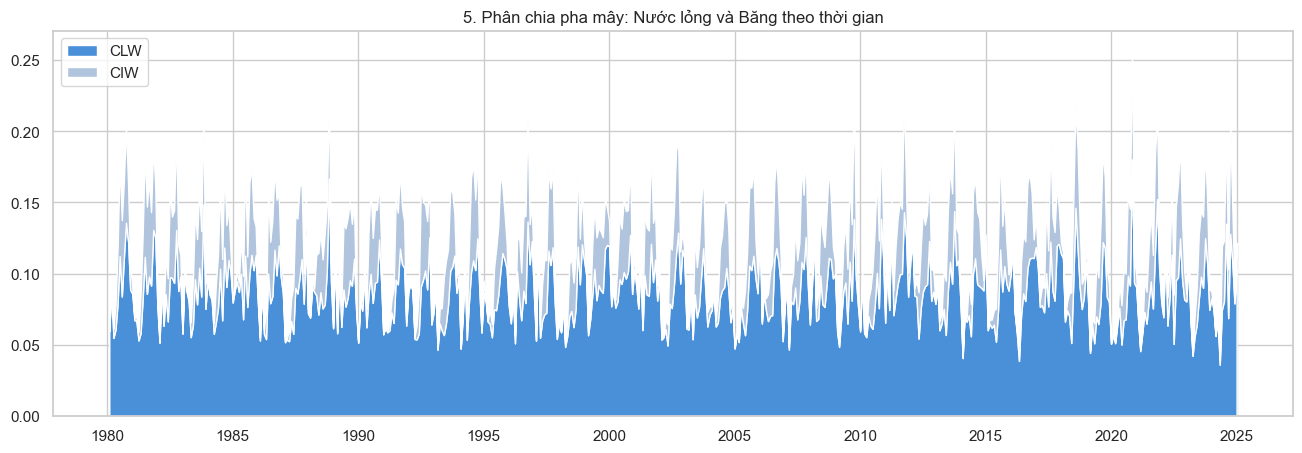
\includegraphics[width=\textwidth]{images/3.4.5.png}
        \caption{Phân chia pha mây CLW/CIW}
    \end{subfigure}
    \hfill
    \begin{subfigure}[b]{0.48\textwidth}
        \centering
        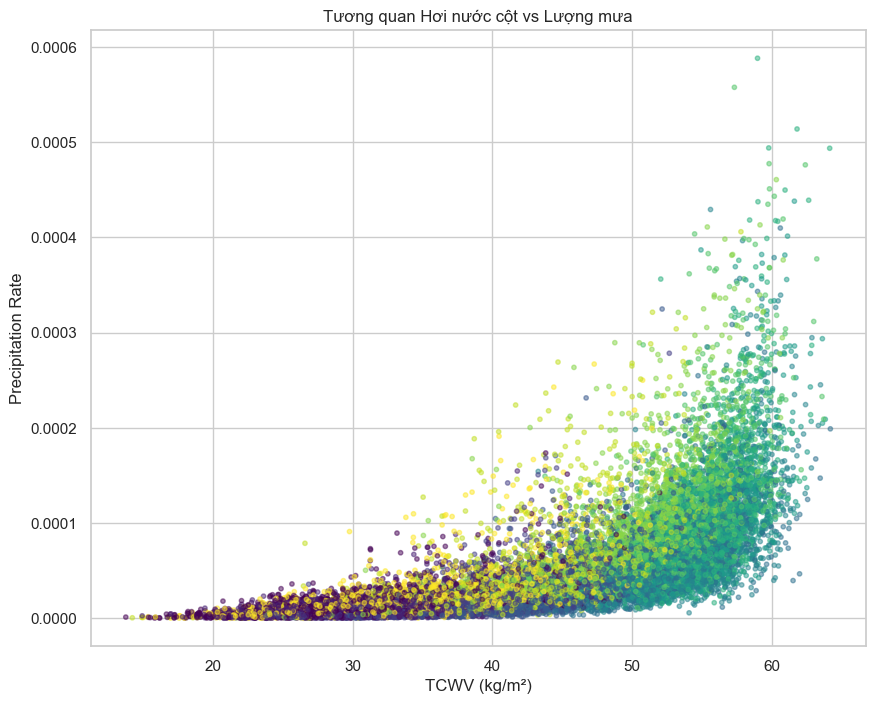
\includegraphics[width=\textwidth]{images/3.4.6.png}
        \caption{Tương quan TCWV vs Mưa}
    \end{subfigure}
    \caption{Động lực thành phần pha mây và kiểm định vật lý giới hạn kích phát mưa}
    \label{fig:cloud_phase_scatter}
\end{figure}
\FloatBarrier

\subsection{Lượng mưa}

\subsubsection{Khí hậu học lượng mưa theo mùa}
Chu kỳ mưa trung bình mùa được thể hiện tại \textbf{Hình \ref{fig:precip_cycle_annual}(a)} minh chứng tính chất mưa đặc thù khu vực.

\begin{itemize}
    \item \textbf{Đặc trưng khí hậu (RQ1):} Lượng mưa miền Trung có đặc trưng "lệch muộn" cực kỳ rõ nét, bắt đầu tăng mạnh từ tháng 5 và đạt đỉnh cao nhất vào tháng 9 (~10 mm/ngày). Mưa đối lưu luôn chiếm tỷ trọng chủ đạo xuyên suốt cả năm, duy trì nguồn cung nước chính cho mặt đệm.
    \item \textbf{Tác nhân khắc nghiệt (RQ2):} Đỉnh mưa cực đại tháng 9--10 là hệ quả từ sự tương tác khốc liệt giữa bão, dải hội tụ ITCZ và địa hình dốc của dãy Trường Sơn. Sự kết hợp các tác nhân này giải phóng lượng ẩm khổng lồ thành mưa lũ thảm khốc trong thời gian cực ngắn.
\end{itemize}

\subsubsection{Biến động lượng mưa tổng cộng hàng năm}
Dựa trên chuỗi số liệu tại \textbf{Hình \ref{fig:precip_cycle_annual}(b)}, lượng mưa năm miền Trung thể hiện tính bất ổn định cao.

\begin{itemize}
    \item \textbf{Đặc trưng khí hậu (RQ1):} Lượng mưa năm dao động rất rộng giữa các năm, từ mức 1500 mm đến trên 2100 mm. Tính biến động liên năm mạnh mẽ này xác lập đặc trưng khí hậu miền Trung là khu vực nhạy cảm bậc nhất cả nước về thủy văn.
    \item \textbf{Tác nhân khắc nghiệt (RQ2):} Sự trồi sụt thất thường của lượng mưa năm gắn liền chặt chẽ với chu kỳ \textbf{ENSO}. Tác nhân La Niña gây ra các trận lũ lịch sử vượt mọi giới hạn, trong khi El Niño tạo ra hạn hán khắc nghiệt kéo dài làm cạn kiệt sông ngòi.
\end{itemize}

\FloatBarrier
\begin{figure}[H]
    \centering
    \begin{subfigure}[b]{0.48\textwidth}
        \centering
        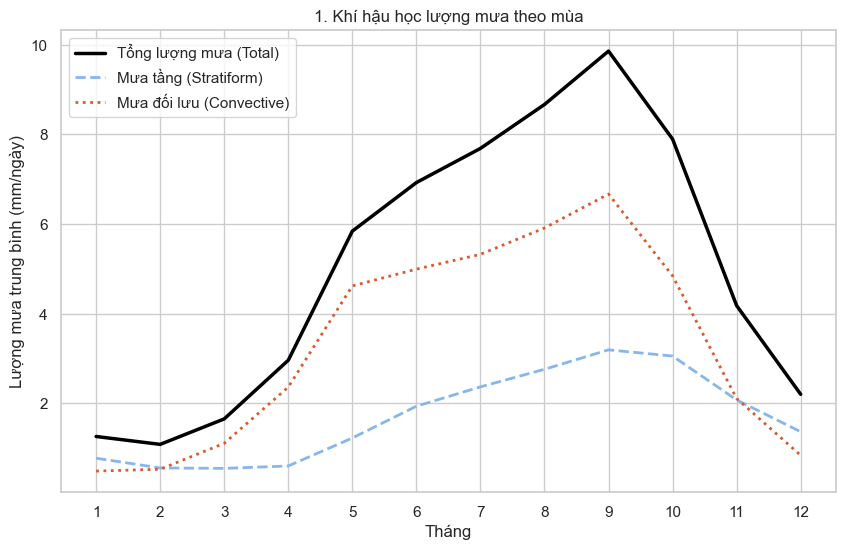
\includegraphics[width=\textwidth]{images/3.5.1.png}
        \caption{Chu kỳ mùa theo loại mưa}
    \end{subfigure}
    \hfill
    \begin{subfigure}[b]{0.48\textwidth}
        \centering
        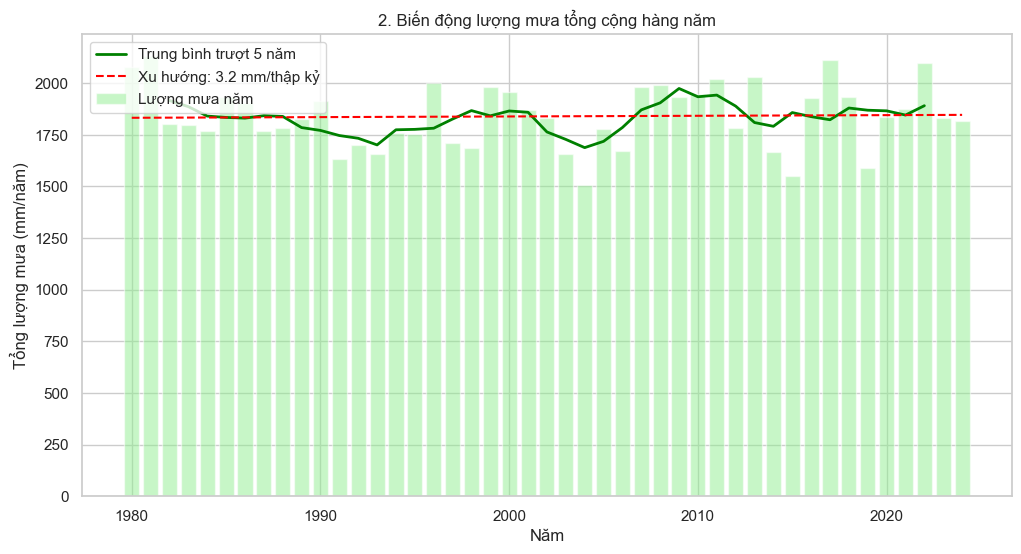
\includegraphics[width=\textwidth]{images/3.5.2.png}
        \caption{Biến động lượng mưa năm}
    \end{subfigure}
    \caption{Phân tích đặc trưng chu kỳ mùa và biên độ biến động lượng mưa miền Trung}
    \label{fig:precip_cycle_annual}
\end{figure}
\FloatBarrier

\subsubsection{Xu hướng tỷ lệ mưa đối lưu (Convective Fraction)}
Dịch chuyển cấu trúc vật lý gây mưa được minh chứng rõ rệt qua xu hướng tại \textbf{Hình \ref{fig:precip_fraction_anomaly}(a)}.

\begin{itemize}
    \item \textbf{Đặc trưng khí hậu (RQ1):} Mưa đối lưu đóng góp khoảng 68% nhưng đang có xu hướng giảm nhẹ (-0.0063/thập kỷ) nhường chỗ cho mưa tầng diện rộng. Đặc trưng này phản ánh một sự chuyển dịch âm thầm trong bản chất của các trận mưa tại khu vực miền Trung.
    \item \textbf{Tác nhân khắc nghiệt (RQ2):} Việc gia tăng tỷ trọng mưa tầng diện rộng kết hợp địa hình \textbf{Trường Sơn} làm kéo dài thời gian ngập lụt tại các lưu vực sông. Tác nhân mưa tầng bão hòa ẩm địa chất lâu ngày là nguyên nhân chính gây ra các đợt sạt lở đất đá thảm khốc tại vùng núi.
\end{itemize}

\subsubsection{Ma trận dị thường lượng mưa hàng tháng}
Tính chất cực đoan hóa lượng mưa qua ma trận tại \textbf{Hình \ref{fig:precip_fraction_anomaly}(b)} ghi lại những năm thiên tai trọng điểm.

\begin{itemize}
    \item \textbf{Đặc trưng khí hậu (RQ1):} Ma trận phản ánh sự xuất hiện đột ngột và bất quy luật của dị thường dương (xanh - mưa rất to) và dị thường âm (nâu - hạn hán). Đặc trưng khí hậu miền Trung đang trở nên khó dự báo hơn khi các mảng dị thường xuất hiện dày đặc.
    \item \textbf{Tác nhân khắc nghiệt (RQ2):} Vệt xanh đậm cuối năm (như năm 2020) minh chứng tác nhân bão chồng bão khốc liệt đánh bại khả năng tiêu thoát nước hạ tầng. Ngược lại, mảng nâu đỏ phản ánh sức tàn phá của El Niño làm triệt tiêu mùa mưa truyền thống.
\end{itemize}

\FloatBarrier
\begin{figure}[H]
    \centering
    \begin{subfigure}[b]{0.48\textwidth}
        \centering
        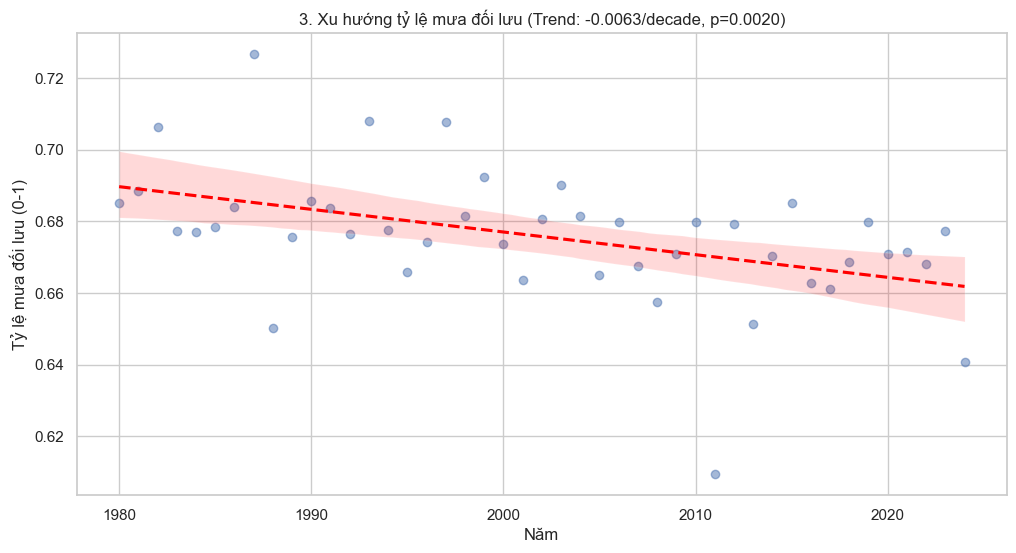
\includegraphics[width=\textwidth]{images/3.5.3.png}
        \caption{Xu hướng tỷ lệ mưa đối lưu}
    \end{subfigure}
    \hfill
    \begin{subfigure}[b]{0.48\textwidth}
        \centering
        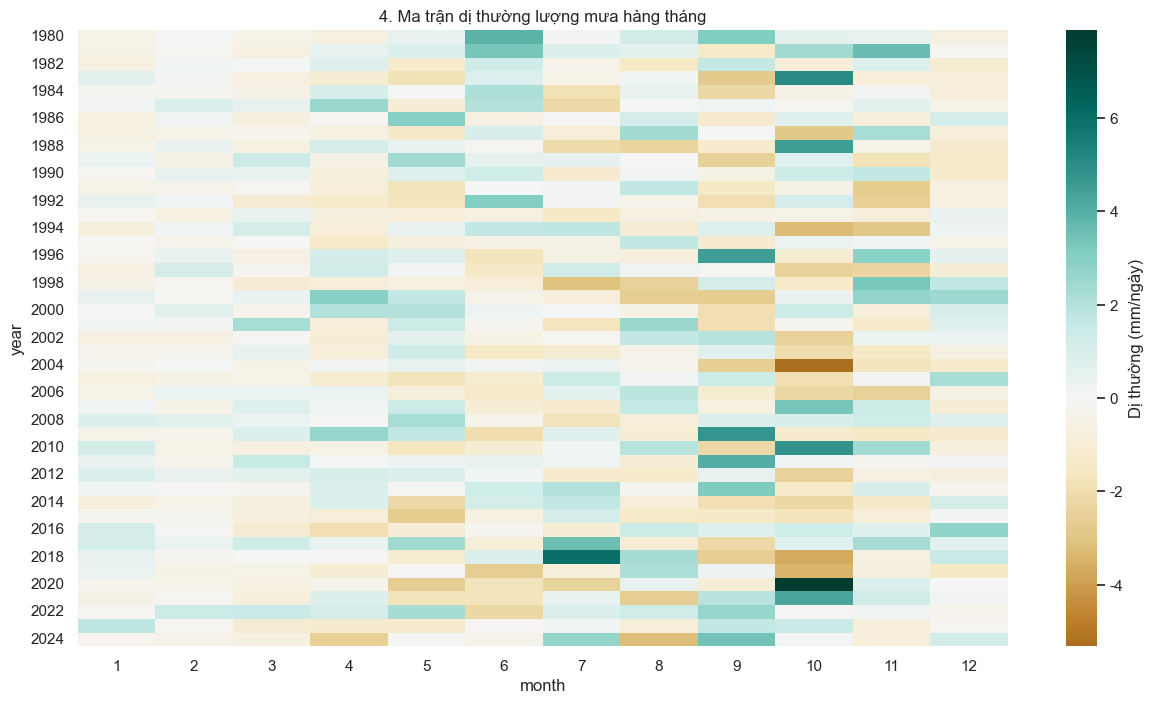
\includegraphics[width=\textwidth]{images/3.5.4.png}
        \caption{Ma trận dị thường lượng mưa}
    \end{subfigure}
    \caption{Phân tích dịch chuyển tính chất mưa và ma trận dị thường hàng tháng lịch sử}
    \label{fig:precip_fraction_anomaly}
\end{figure}
\FloatBarrier

\subsubsection{Phân hóa tính chất mưa: Đối lưu vs Tầng}
Xung đột tính chất mưa tại \textbf{Hình \ref{fig:precip_type_threshold}(a)} mô tả động lực phức tạp của các đợt mưa lớn.

\begin{itemize}
    \item \textbf{Đặc trưng khí hậu (RQ1):} Mưa miền Trung là sự đan xen liên tục giữa các xung đối lưu ngắn hạn cường độ cao và các đợt mưa tầng bão hòa kéo dài. Đặc trưng hỗn hợp này biến khu vực thành một trong những điểm nóng mưa lũ phức tạp nhất thế giới nhiệt đới.
    \item \textbf{Tác nhân khắc nghiệt (RQ2):} Sự cộng hưởng đồng thời cả hai loại mưa trong mùa bão lũ chính là tác nhân đẩy rủi ro thiên tai lên mức cực hạn. Mưa đối lưu gây lũ quét cục bộ, trong khi mưa tầng gây ngập lụt diện rộng kéo dài nhiều tuần.
\end{itemize}

\subsubsection{Tần suất các ngày mưa cực đoan theo ngưỡng}
Biến động cực trị mưa vượt ngưỡng tại \textbf{Hình \ref{fig:precip_type_threshold}(b)} lượng hóa rủi ro thiên tai liên năm.

\begin{itemize}
    \item \textbf{Đặc trưng khí hậu (RQ1):} Những ngày mưa rất to ($>40$mm) dù tần suất thấp nhưng lại quyết định hoàn toàn trữ lượng nước và rủi ro lũ lụt của cả năm. Số lượng ngày cực đoan này có biên độ dao động mạnh nhất trong các ngưỡng mưa nghiên cứu.
    \item \textbf{Tác nhân khắc nghiệt (RQ2):} Tần suất mưa R40mm tăng vọt minh chứng cho sự \textbf{cực đoan hóa khí hậu} do nhiệt độ biển tăng nén ẩm mạnh hơn. Tác nhân này khiến miền Trung đối mặt với các trận mưa cường suất lớn thường xuyên hơn, đe dọa sự an toàn của các công trình hồ đập.
\end{itemize}

\FloatBarrier
\begin{figure}[H]
    \centering
    \begin{subfigure}[b]{0.48\textwidth}
        \centering
        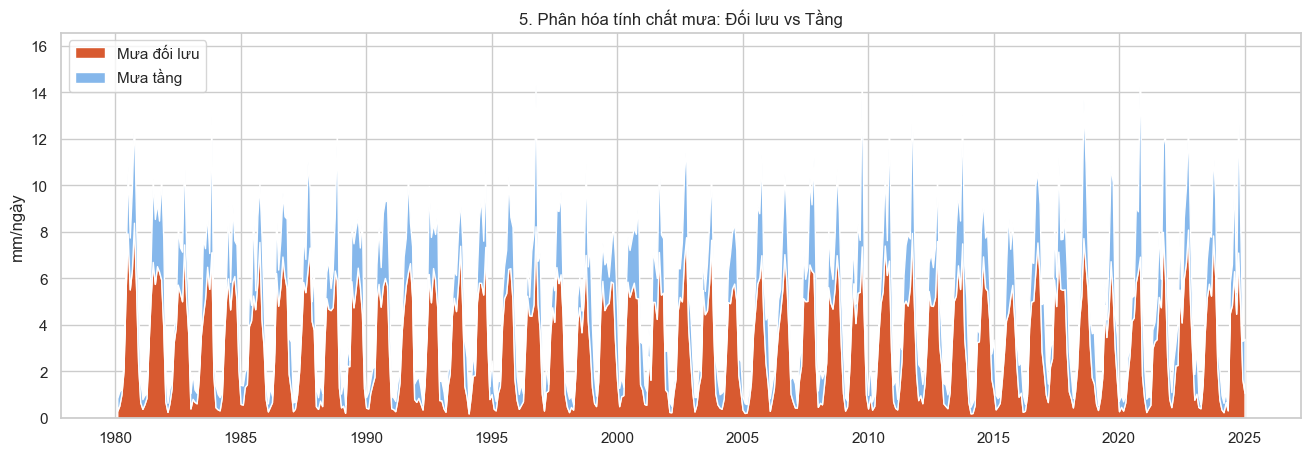
\includegraphics[width=\textwidth]{images/3.5.5.png}
        \caption{Diễn biến Đối lưu vs Tầng}
    \end{subfigure}
    \hfill
    \begin{subfigure}[b]{0.48\textwidth}
        \centering
        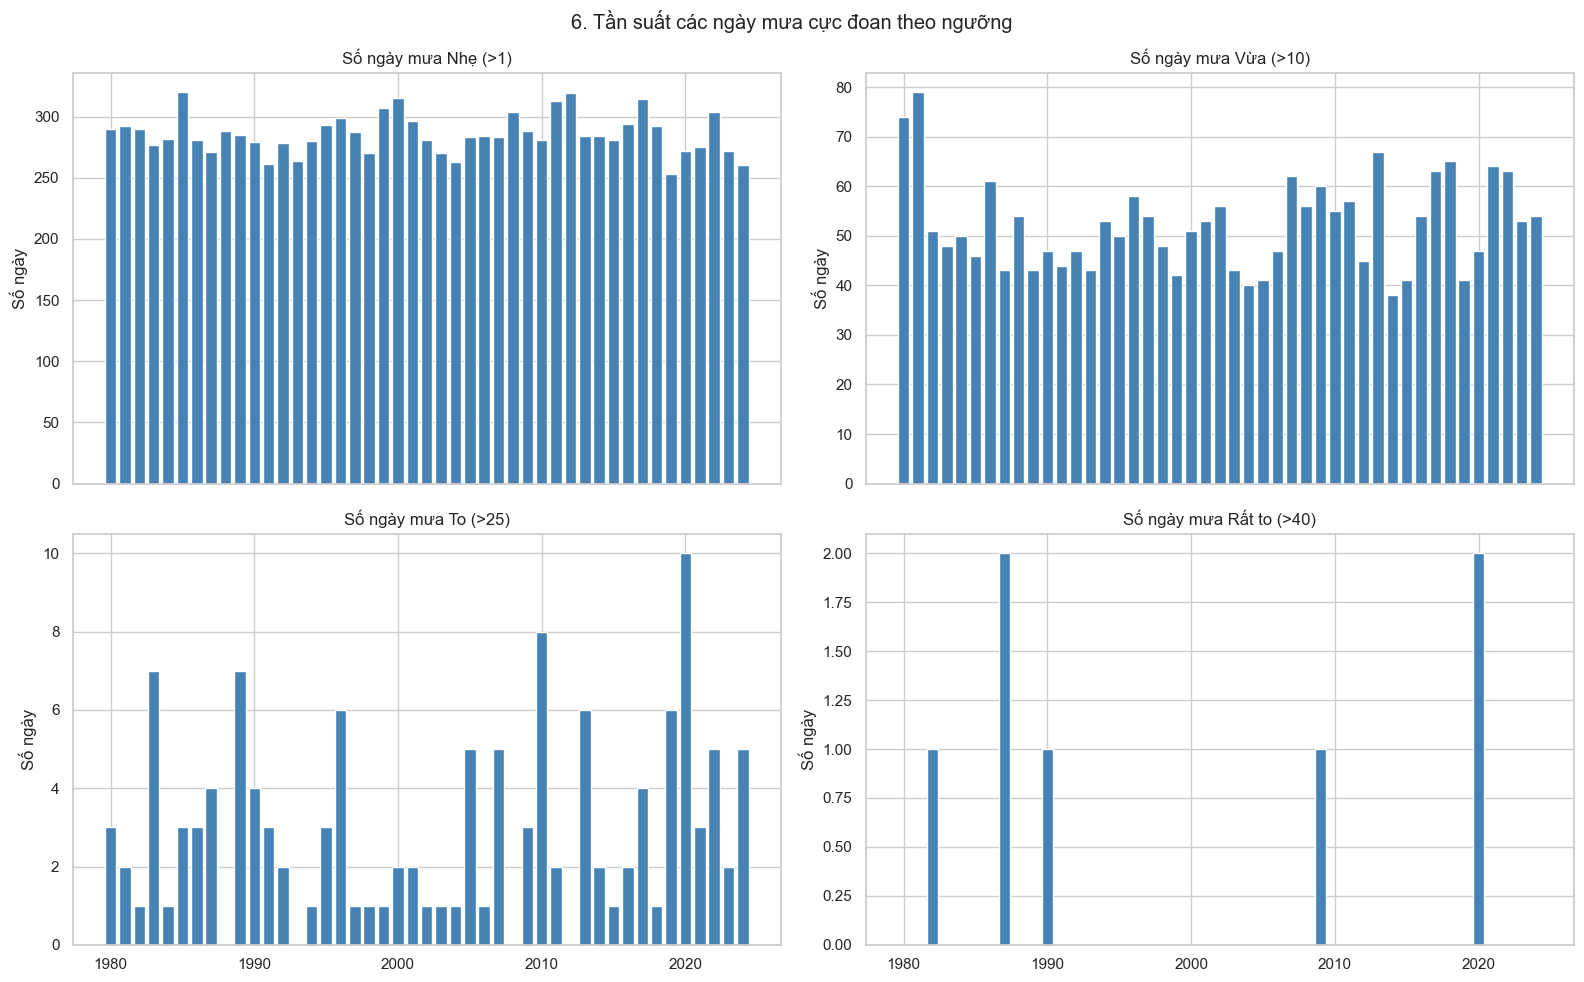
\includegraphics[width=\textwidth]{images/3.5.6.png}
        \caption{Tần suất mưa theo ngưỡng}
    \end{subfigure}
    \caption{Phân tích động lực cấu trúc mưa và phân bổ tần suất cực trị vượt ngưỡng}
    \label{fig:precip_type_threshold}
\end{figure}
\FloatBarrier

\subsubsection{Sự dịch chuyển phân phối lượng mưa theo thập kỷ (ECDF)}
Hàm phân phối tích lũy tại \textbf{Hình \ref{fig:precip_ecdf_dry}(a)} xác nhận sự thay đổi cấu trúc xác suất các trận mưa.

\begin{itemize}
    \item \textbf{Đặc trưng khí hậu (RQ1):} Đường cong ECDF của thập kỷ 2020 lệch phải rõ rệt ở vùng cường độ cao, khẳng định mưa đang trở nên nặng hạt hơn. Đặc trưng "mưa to hơn trong thời gian ngắn" ngày càng phổ biến trong cấu trúc thời tiết miền Trung.
    \item \textbf{Tác nhân khắc nghiệt (RQ2):} Sự dịch chuyển này là minh chứng cho việc biến đổi khí hậu làm gia tăng khả năng giải phóng năng lượng ẩm cực bộ. Tác nhân này trực tiếp làm trầm trọng hóa bài toán thoát lũ cho các đô thị ven biển miền Trung trong thập kỷ qua.
\end{itemize}

\subsubsection{Độ dài đợt khô hạn nhất trong năm (Dry Spell Length)}
Chu kỳ khô hạn khắc nghiệt được thể hiện qua chuỗi thời gian tại \textbf{Hình \ref{fig:precip_ecdf_dry}(b)}.

\begin{itemize}
    \item \textbf{Đặc trưng khí hậu (RQ1):} Khu vực thường chịu các đợt không mưa kéo dài liên tục từ 10 đến 30 ngày, xác lập ranh giới mùa khô - mùa mưa vô cùng gắt gao. Đặc trưng này gây áp lực cực lớn lên việc dự trữ và điều tiết nguồn nước mặt.
    \item \textbf{Tác nhân khắc nghiệt (RQ2):} Các đợt hạn hán dài ngày ($>25$ ngày) thường do tác nhân \textbf{gió Lào} nung nóng bề mặt và sự thiếu hụt bão từ đại dương. Tác nhân khô nóng bền bỉ này làm kiệt quệ nguồn nước tầng nông, trực tiếp đe dọa sự sống của hệ sinh thái nông nghiệp khu vực.
\end{itemize}

\FloatBarrier
\begin{figure}[H]
    \centering
    \begin{subfigure}[b]{0.48\textwidth}
        \centering
        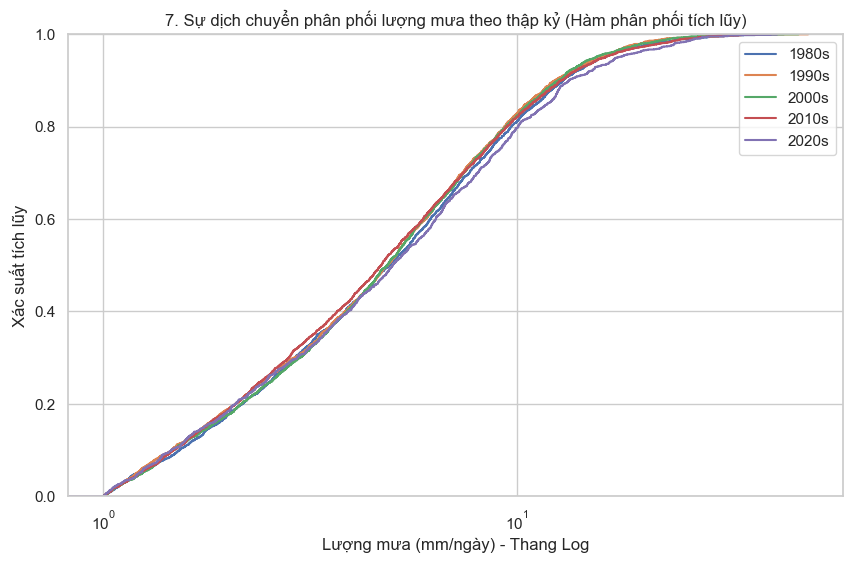
\includegraphics[width=\textwidth]{images/3.5.7.png}
        \caption{Hàm phân phối tích lũy ECDF}
    \end{subfigure}
    \hfill
    \begin{subfigure}[b]{0.48\textwidth}
        \centering
        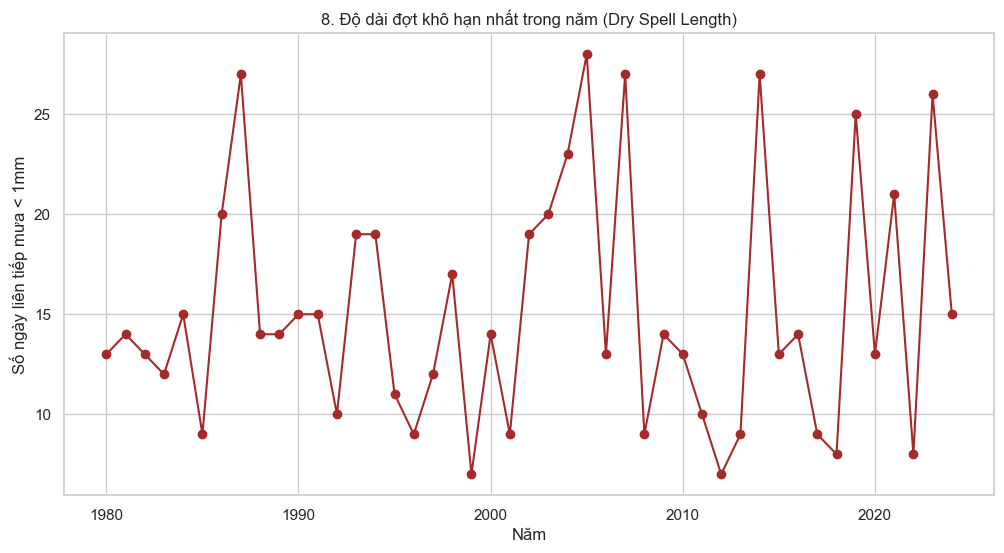
\includegraphics[width=\textwidth]{images/3.5.8.png}
        \caption{Độ dài đợt khô hạn nhất}
    \end{subfigure}
    \caption{Phân tích dịch chuyển xác suất mưa và động lực chu kỳ khô hạn liên năm}
    \label{fig:precip_ecdf_dry}
\end{figure}
\FloatBarrier

\subsection{Bốc hơi}

\subsubsection{Lượng bốc hơi thực tế và lượng bốc hơi tiềm năng}
Cân bằng bốc hơi tại \textbf{Hình \ref{fig:evap_cycle_stress}(a)} cho thấy thâm hụt nước khổng lồ vào nửa đầu năm.

\begin{itemize}
    \item \textbf{Đặc trưng khí hậu (RQ1):} Nhu cầu bốc hơi khí quyển ($E_p$) luôn vượt xa khả năng cung cấp ẩm thực tế ($E$) từ đất vào các tháng 1--5. Đặc trưng này xác lập giai đoạn thâm hụt nước sinh lý cực đoan cho toàn bộ thảm thực vật miền Trung trước khi mùa mưa bắt đầu.
    \item \textbf{Tác nhân khắc nghiệt (RQ2):} Tác nhân \textbf{gió Lào} đẩy nhu cầu hút ẩm $E_p$ lên ngưỡng cực hạn, nén chặt độ ẩm mặt đệm trong bối cảnh thiếu hụt mưa. Sự kết hợp này kích phát trạng thái hạn hán nông nghiệp nghiêm trọng, làm suy kiệt độ ẩm tích lũy của đất rừng.
\end{itemize}

\subsubsection{Mức độ căng thẳng của nước}
Dựa trên chỉ số tại \textbf{Hình \ref{fig:evap_cycle_stress}(b)}, đỉnh điểm căng thẳng nước tháng 3 xác lập ranh giới sinh tồn của hệ sinh thái.

\begin{itemize}
    \item \textbf{Đặc trưng khí hậu (RQ1):} Chỉ số căng thẳng nước đạt cực đại tháng 3 (~1.5) minh chứng tính chất khô hạn đặc hữu của dải ven biển. Đặc trưng này cho thấy sự mâu thuẫn gay gắt giữa nhu cầu sinh trưởng của cây trồng và khả năng đáp ứng ẩm của khí quyển.
    \item \textbf{Tác nhân khắc nghiệt (RQ2):} Khối khí lục địa khô kết hợp bức xạ tăng cường là tác nhân nới rộng vùng thâm hụt nước bề mặt. Tình trạng căng thẳng nước kéo dài là nguyên nhân trực tiếp dẫn đến nguy cơ cháy rừng cao độ tại vùng phía Tây miền Trung.
\end{itemize}

\FloatBarrier
\begin{figure}[H]
    \centering
    \begin{subfigure}[b]{0.48\textwidth}
        \centering
        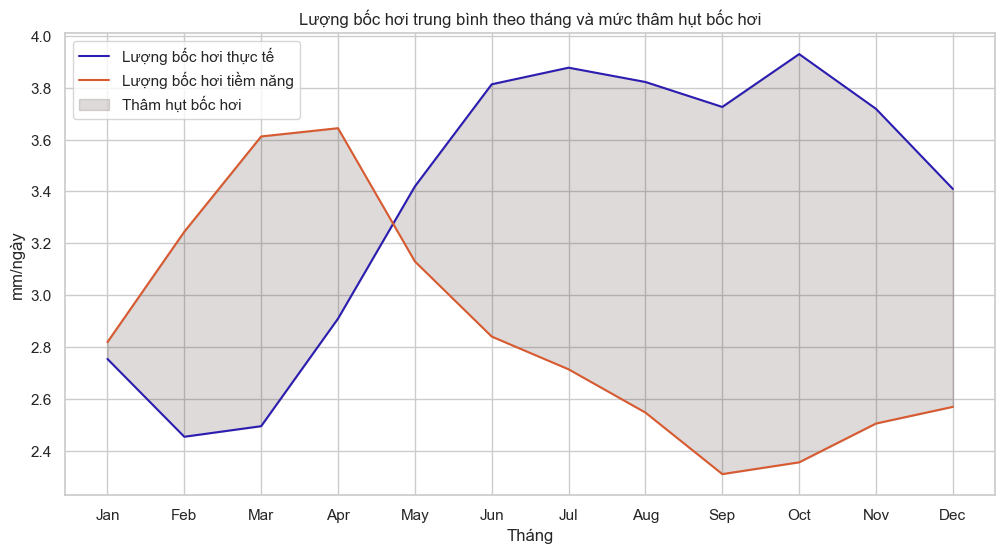
\includegraphics[width=\textwidth]{images/3.6.1.png}
        \caption{Cân bằng bốc hơi theo tháng}
    \end{subfigure}
    \hfill
    \begin{subfigure}[b]{0.48\textwidth}
        \centering
        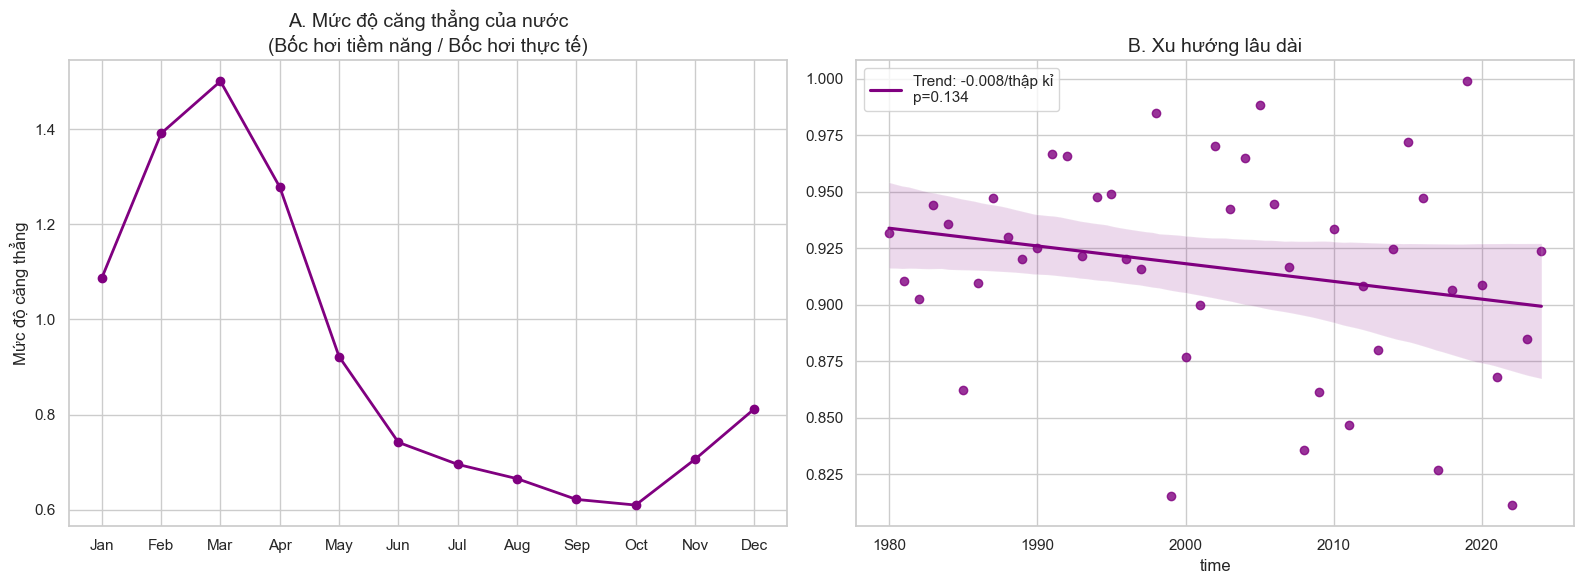
\includegraphics[width=\textwidth]{images/3.6.5.png}
        \caption{Mức độ căng thẳng nước}
    \end{subfigure}
    \caption{Phân tích đặc trưng nhu cầu ẩm khí quyển và trạng thái căng thẳng nước bề mặt}
    \label{fig:evap_cycle_stress}
\end{figure}
\FloatBarrier

\subsubsection{Chu kỳ mùa và xu hướng dài hạn của hệ số bốc hơi}
Dịch chuyển hệ số EF tại \textbf{Hình \ref{fig:evap_ef_trend}(a)} phản ánh độ khô kiệt mặt đệm cực đoan tháng 3.

\begin{itemize}
    \item \textbf{Đặc trưng khí hậu (RQ1):} Hệ số EF thấp nhất (~0.7) vào mùa khô khẳng định đặc tính thổ nhưỡng khu vực rất dễ mất ẩm mặt đệm. Trạng thái bão hòa EF bám sát mùa mưa bão, xác lập chu trình thủy văn mặt đất vô cùng nhạy bén với hoàn lưu gió mùa.
    \item \textbf{Tác nhân khắc nghiệt (RQ2):} Sự sụt giảm đột ngột EF trong các chu kỳ El Niño mạnh là minh chứng cho sự khắc nghiệt của tình trạng hạn hán quy mô vùng. Tác nhân biến động liên năm làm suy yếu khả năng cung cấp ẩm thực tế của đất, đẩy EF xuống ngưỡng nguy hiểm cho nông nghiệp.
\end{itemize}

\subsubsection{Xu hướng lâu dài bốc hơi thực tế/tiềm năng}
Tăng cường chu trình thủy văn tại \textbf{Hình \ref{fig:evap_ef_trend}(b)} với tốc độ tăng bốc hơi thực tế $E$ rất mạnh.

\begin{itemize}
    \item \textbf{Đặc trưng khí hậu (RQ1):} Vòng tuần hoàn nước miền Trung đang diễn ra nhanh hơn với lượng bay hơi thực tế tăng +0.0351 mm/ngày/thập kỷ. Đặc trưng này cho thấy bề mặt miền Trung đang giải phóng hơi nước mãnh liệt hơn vào khí quyển bối cảnh ấm hóa.
    \item \textbf{Tác nhân khắc nghiệt (RQ2):} Nhiệt độ tăng mạnh là tác nhân trực tiếp nung nóng mặt đệm và Biển Đông, kích phát bốc hơi mạnh. Bay hơi thực tế tăng nhanh làm trầm trọng hóa sự kiệt quệ độ ẩm rễ cây sau mỗi đợt sóng nhiệt, làm giảm khả năng phục hồi của thảm xanh.
\end{itemize}

\FloatBarrier
\begin{figure}[H]
    \centering
    \begin{subfigure}[b]{0.48\textwidth}
        \centering
        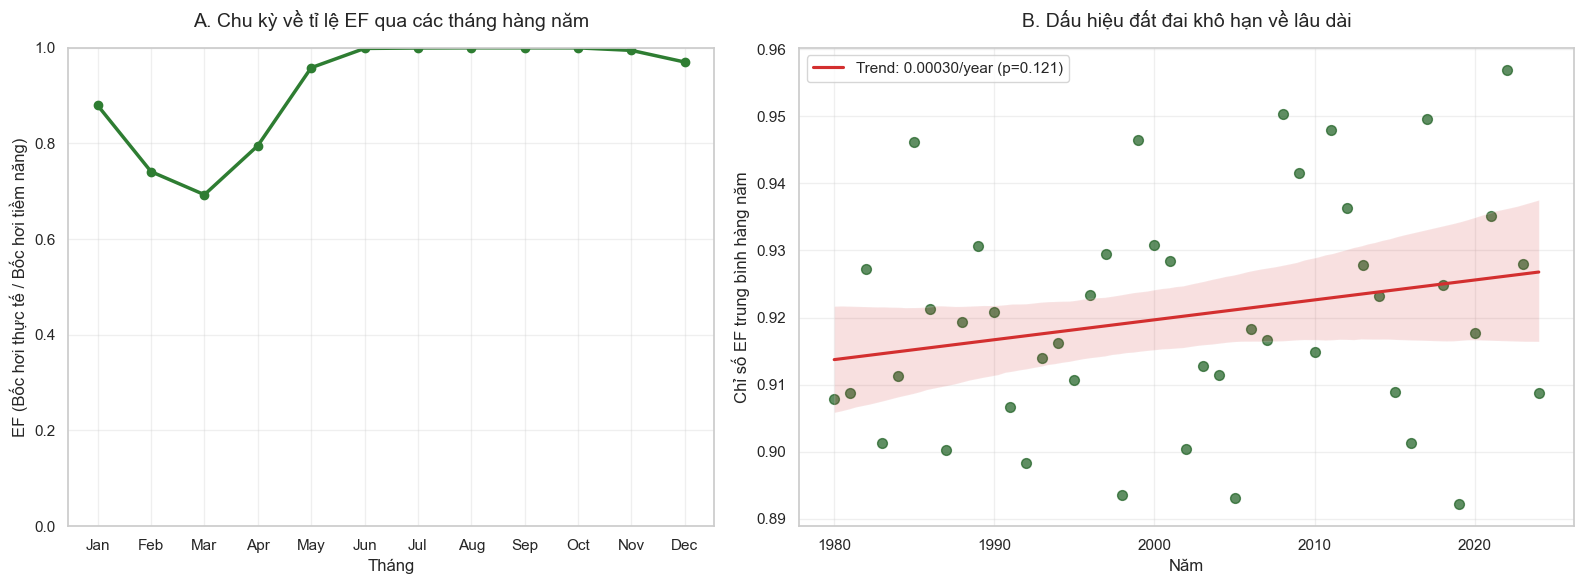
\includegraphics[width=\textwidth]{images/3.6.2.png}
        \caption{Hệ số bốc hơi EF}
    \end{subfigure}
    \hfill
    \begin{subfigure}[b]{0.48\textwidth}
        \centering
        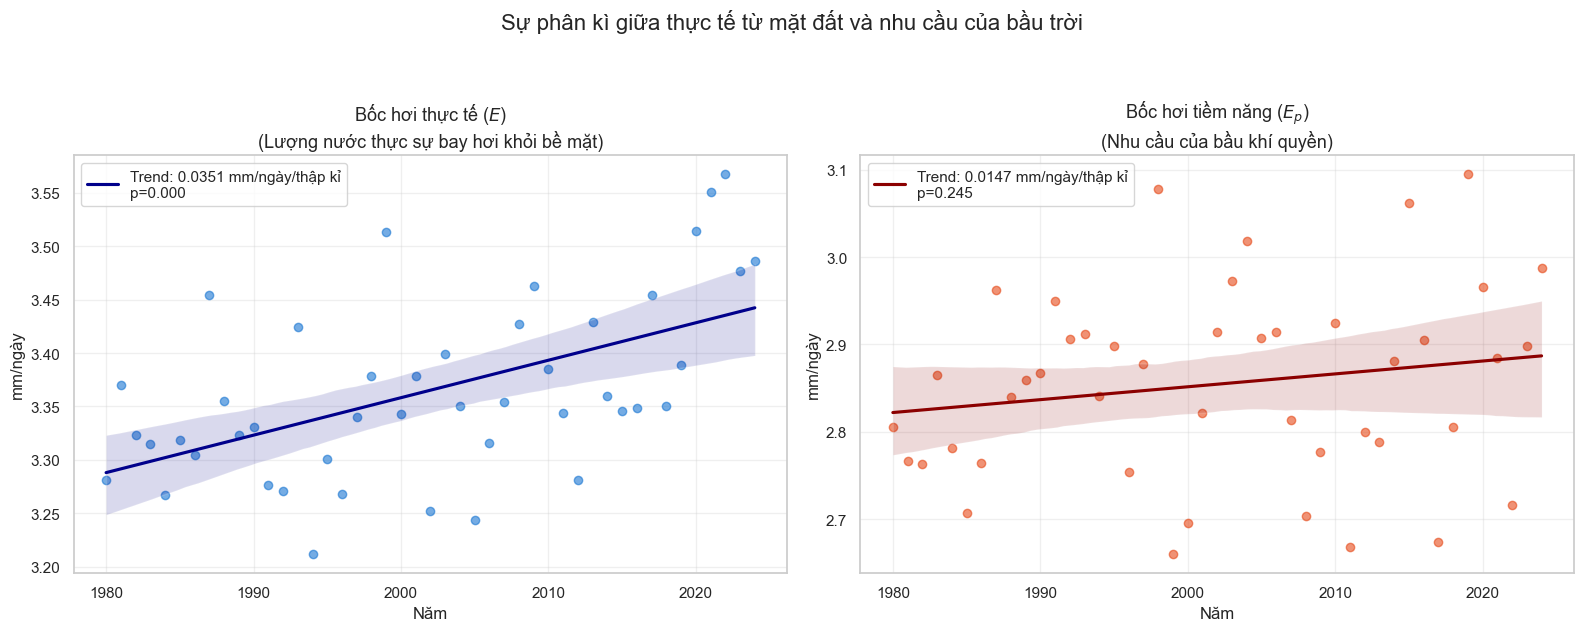
\includegraphics[width=\textwidth]{images/3.6.4.png}
        \caption{Xu hướng dài hạn bốc hơi}
    \end{subfigure}
    \caption{Phân tích động lực hệ số EF và xu hướng tăng cường chu trình nước mặt đệm}
    \label{fig:evap_ef_trend}
\end{figure}
\FloatBarrier

\subsubsection{Heatmap mức độ thâm hụt bốc hơi qua các tháng trong các năm}
Ma trận thâm hụt tại \textbf{Hình \ref{fig:evap_deficit_heatmap}} ghi dấu ấn khô hạn lịch sử định kỳ vào các tháng 4--5.

\begin{itemize}
    \item \textbf{Đặc trưng khí hậu (RQ1):} Các chu kỳ khô hạn đỏ đậm tập trung nửa đầu năm và ngày càng xuất hiện với cường độ cao hơn từ sau năm 2014. Đặc trưng này xác lập tính chất thâm hụt ẩm bầu trời ngày càng khắc nghiệt hơn qua từng năm.
    \item \textbf{Tác nhân khắc nghiệt (RQ2):} Các năm thâm hụt cực đại gắn liền với tác nhân \textbf{El Niño mạnh} (1998, 2016, 2024). Sự thiếu hụt nước bầu trời đầu hè là nguyên nhân kích phát các trận cháy rừng quy mô lớn tàn phá hệ sinh thái rừng Trường Sơn.
\end{itemize}

\FloatBarrier
\begin{figure}[H]
    \centering
    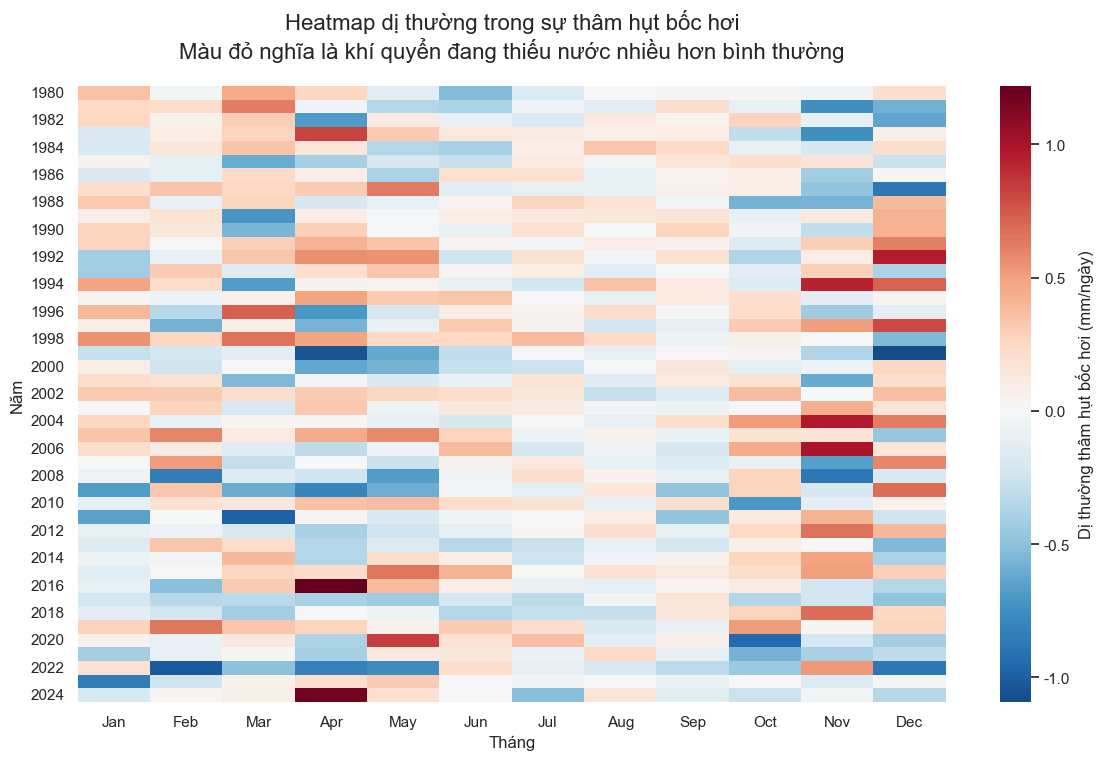
\includegraphics[width=0.7\textwidth]{images/3.6.3.png}
    \caption{Ma trận dị thường thâm hụt bốc hơi hàng tháng (1980--2024)}
    \label{fig:evap_deficit_heatmap}
\end{figure}
\FloatBarrier

\subsubsection{So sánh sự phân bố theo từng thập kỷ}
Dịch chuyển mật độ tại \textbf{Hình \ref{fig:evap_violin}} cho thấy dải bốc hơi thực tế đang dâng cao hệ thống qua các thập kỷ.

\begin{itemize}
    \item \textbf{Đặc trưng khí hậu (RQ1):} Hình dáng phân phối mở rộng rõ rệt ở phần đỉnh trong mùa mưa, khẳng định các sự kiện bốc hơi cường độ cao xuất hiện ngày càng thường xuyên. Sự chuyển dịch tịnh tiến của các hộp phân phối là minh chứng cho biến đổi khí hậu đang làm nóng dần chu trình nước.
    \item \textbf{Tác nhân khắc nghiệt (RQ2):} Tác động từ nhiệt độ bề mặt \textbf{Biển Đông} tăng cao khiến miền Trung chịu bốc hơi mạnh ngay sau khi kết thúc các đợt mưa bão. Tác nhân này làm xáo trộn cân bằng năng lượng bề mặt, tăng cảm giác oi bức thực tế sau các thiên tai mưa lũ.
\end{itemize}

\FloatBarrier
\begin{figure}[H]
    \centering
    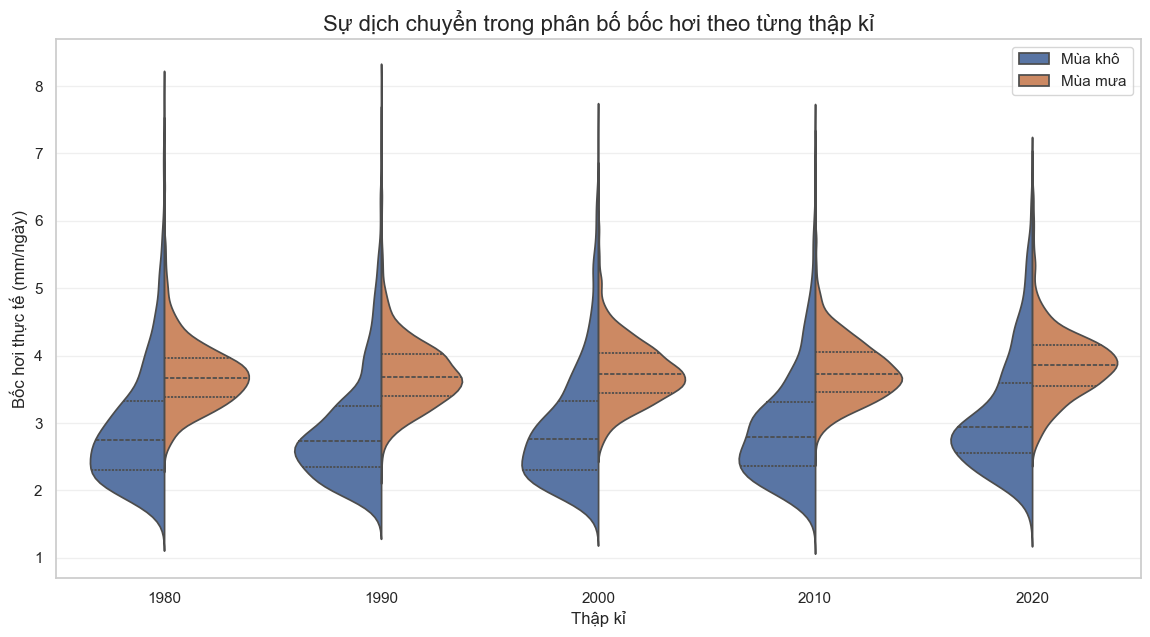
\includegraphics[width=0.7\textwidth]{images/3.6.6.png}
    \caption{Phân phối mật độ bốc hơi thực tế qua các thập kỷ}
    \label{fig:evap_violin}
\end{figure}
\FloatBarrier

\subsection{Độ ẩm đất}

\subsubsection{Chỉ số độ ẩm của đất trên từng tầng và theo độ sâu}
Phân bổ ẩm địa tầng theo chu kỳ mùa được trình bày chi tiết tại cụm \textbf{Hình \ref{fig:soil_moisture_overview}}.

\begin{itemize}
    \item \textbf{Đặc trưng khí hậu (RQ1):} Độ ẩm đạt đáy tháng 2--3 (~0.19 $m^3/m^3$ ở tầng mặt) và đạt đỉnh tháng 9--10 bão hòa ẩm. Tầng sâu 289cm trễ pha đạt đỉnh vào cuối năm, xác lập đặc trưng điều hòa hơi nước lâu dài của địa tầng miền Trung.
    \item \textbf{Tác nhân khắc nghiệt (RQ2):} Sụt giảm độ ẩm tầng mặt tháng 3 là kết quả của việc thiếu mưa kết hợp \textbf{gió Lào} thiêu đốt bề mặt. Trạng thái bão hòa tháng 9--10 do bão lớn đẩy hệ thống thủy văn địa tầng đạt ngưỡng giới hạn gây lũ quét thảm khốc.
\end{itemize}

\FloatBarrier
\begin{figure}[H]
    \centering
    \begin{subfigure}[b]{1\textwidth}
        \centering
        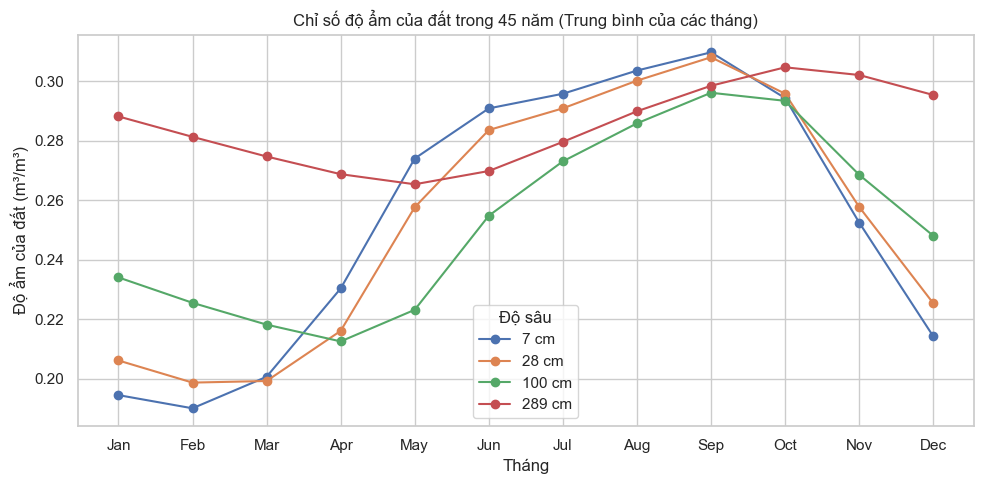
\includegraphics[width=0.7\textwidth]{images/3.7.1.png}
        \caption{Chu kỳ mùa độ ẩm theo tầng}
    \end{subfigure}
    \vspace{8pt}
    \begin{subfigure}[b]{1\textwidth}
        \centering
        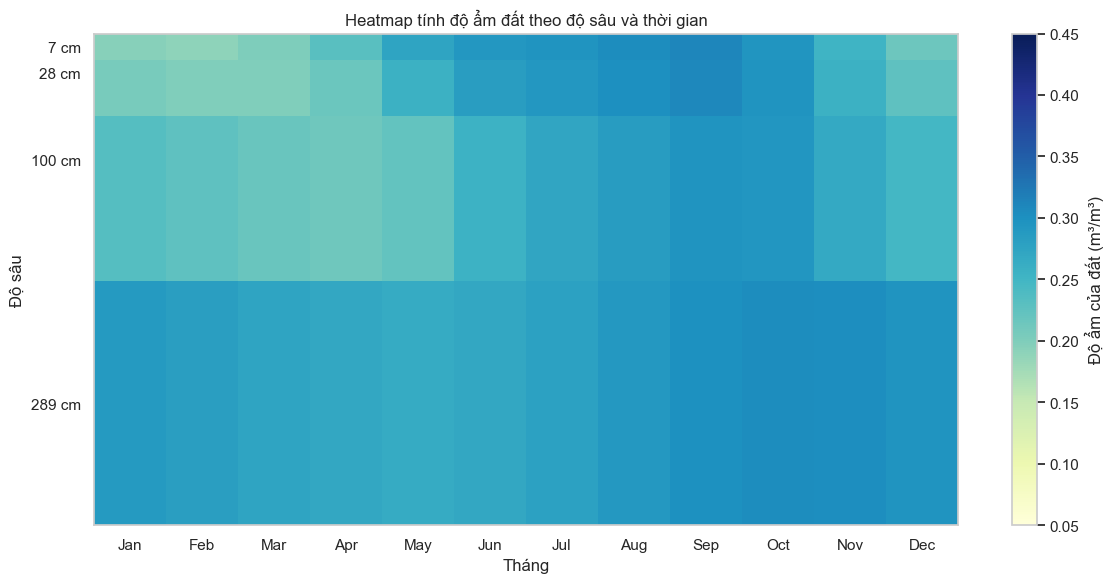
\includegraphics[width=0.7\textwidth]{images/3.7.2.png}
        \caption{Heatmap phân hóa độ sâu theo tháng}
    \end{subfigure}
    \caption{Đặc điểm phân phối độ ẩm đất hệ thống tại miền Trung}
    \label{fig:soil_moisture_overview}
\end{figure}
\FloatBarrier

\subsubsection{Tổng lượng nước trung bình năm \& Ma trận dị thường độ ẩm đất qua các tầng}
Trữ lượng nước đất tại \textbf{Hình \ref{fig:soil_water_series_anomaly}(a)} và dị thường tại \textbf{Hình \ref{fig:soil_water_series_anomaly}(b)} ghi nhận xu hướng khô hạn dài hạn.

\begin{itemize}
    \item \textbf{Đặc trưng khí hậu (RQ1):} Tổng lượng nước cột đất biến động quanh mức 0.79 mét tương đương với biên độ trồi sụt mạnh. Các dị thường đỏ (khô) ngấm sâu xuống tầng 289cm biến địa tầng thành bộ lưu trữ ký ức về thảm họa hạn hán nông nghiệp.
    \item \textbf{Tác nhân khắc nghiệt (RQ2):} Xu hướng giảm nước đất báo hiệu tình trạng \textbf{khô hạn dài hạn} âm thầm diễn ra dưới lòng đất miền Trung. Dị thường âm bao phủ cả 4 tầng (2019-2020) chứng minh thời tiết bề mặt khốc liệt đã hoàn toàn đánh bại khả năng điều tiết thảm phủ.
\end{itemize}

\FloatBarrier
\begin{figure}[H]
    \centering
    \begin{subfigure}[b]{0.48\textwidth}
        \centering
        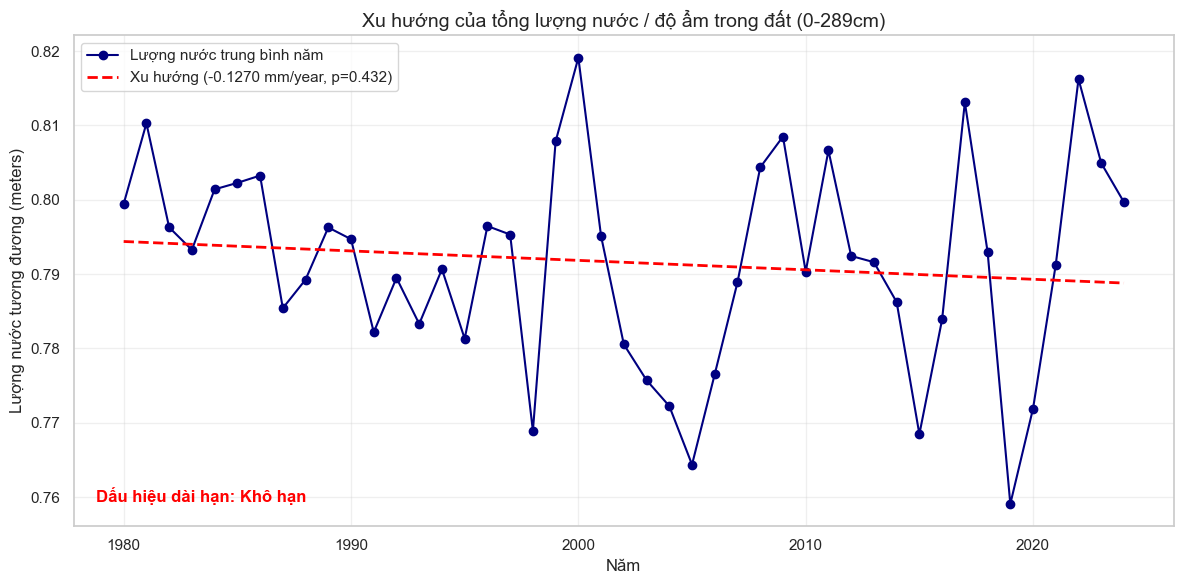
\includegraphics[width=\textwidth]{images/3.7.3.png}
        \caption{Xu hướng tổng lượng nước đất}
    \end{subfigure}
    \hfill
    \begin{subfigure}[b]{0.48\textwidth}
        \centering
        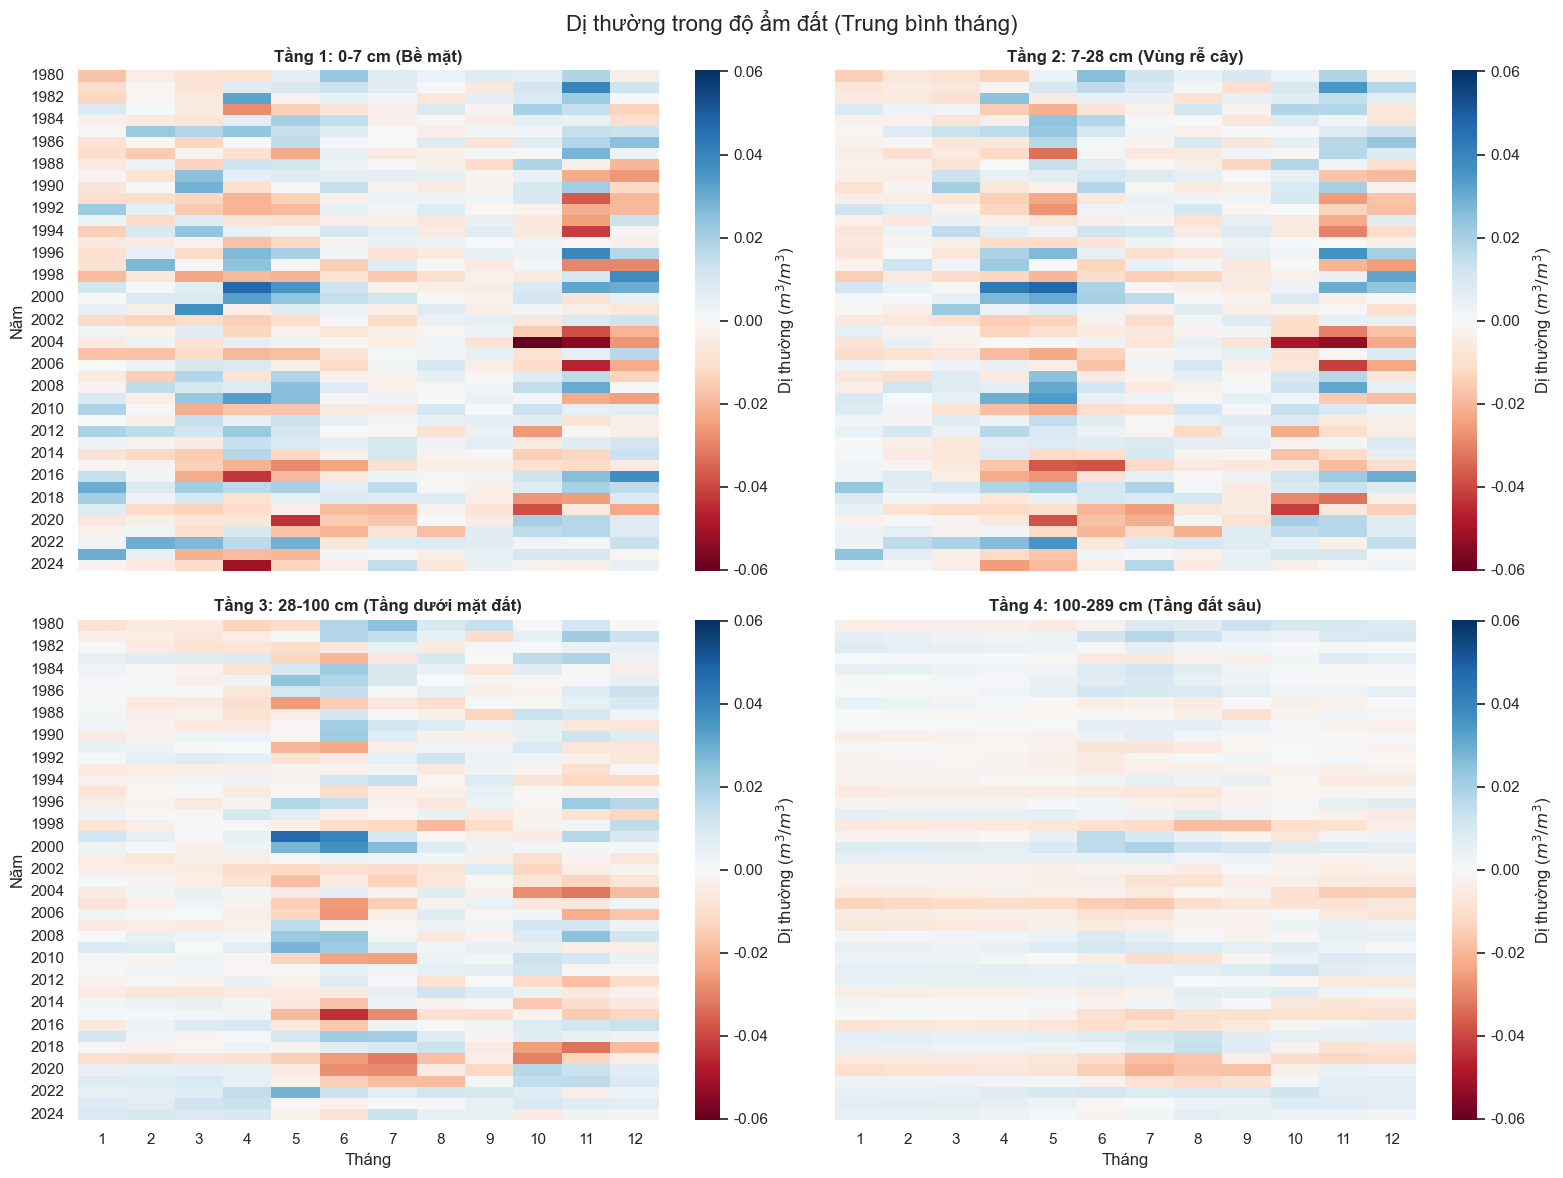
\includegraphics[width=\textwidth]{images/3.7.4.png}
        \caption{Ma trận dị thường ẩm đất}
    \end{subfigure}
    \caption{Phân tích trữ lượng nước địa chất và lan truyền dị thường liên tầng}
    \label{fig:soil_water_series_anomaly}
\end{figure}
\FloatBarrier

\subsubsection{Độ trễ lan truyền ẩm giữa các tầng đất \& Chỉ số độ ẩm đất chuẩn hóa (SSI)}
Động lực thấm ẩm địa tầng tại \textbf{Hình \ref{fig:soil_lag_ssi}(a)} và chu kỳ hạn hán chuẩn hóa tại \textbf{Hình \ref{fig:soil_lag_ssi}(b)}.

\begin{itemize}
    \item \textbf{Đặc trưng khí hậu (RQ1):} Miền Trung cần tới \textbf{39 ngày} để độ ẩm truyền từ độ sâu 1m xuống 2.89m, xác lập độ trễ thủy văn cực lớn. Chỉ số SSI biến động phi quy luật giữa hai thái cực ẩm ướt tuyệt đối và khô hạn kiệt tác, xác lập tính bất ổn định địa tầng.
    \item \textbf{Tác nhân khắc nghiệt (RQ2):} Độ trễ lớn khiến rễ cây bị khô hạn dai dẳng ngay cả khi bề mặt đã có mưa bão. Chỉ số SSI thấp kỷ lục vào các năm 1998, 2019 minh chứng tác nhân \textbf{vô bão} kết hợp nhiệt độ cao làm kiệt quệ tài nguyên nước ngầm nông nghiệp miền Trung.
\end{itemize}

\FloatBarrier
\begin{figure}[H]
    \centering
    \begin{subfigure}[b]{0.48\textwidth}
        \centering
        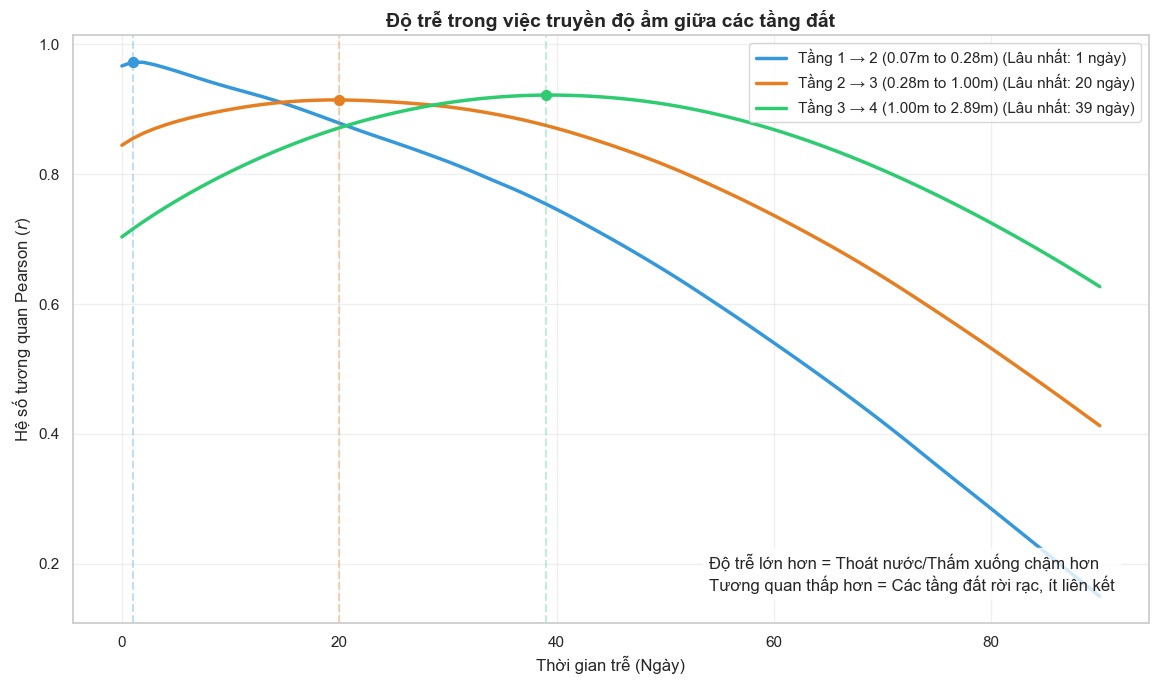
\includegraphics[width=\textwidth]{images/3.7.5.png}
        \caption{Độ trễ truyền ẩm liên tầng}
    \end{subfigure}
    \hfill
    \begin{subfigure}[b]{0.48\textwidth}
        \centering
        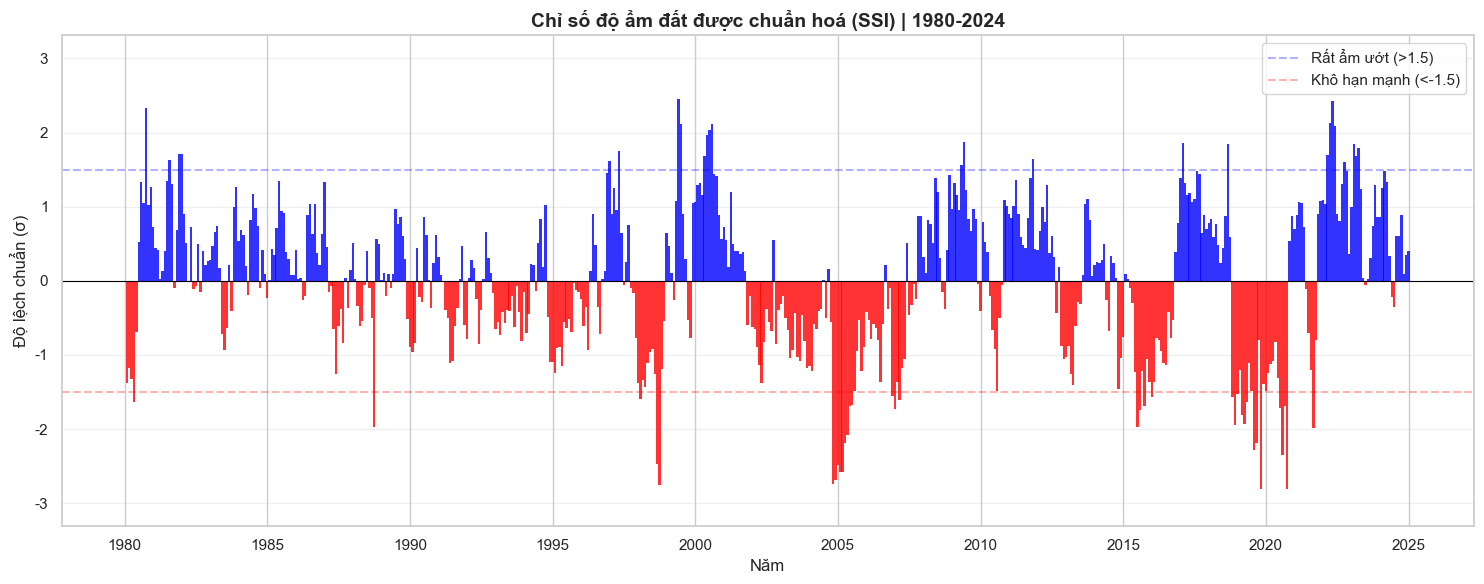
\includegraphics[width=\textwidth]{images/3.7.6.png}
        \caption{Chỉ số SSI (1980--2024)}
    \end{subfigure}
    \caption{Định lượng động lực thấm địa tầng và chu kỳ hạn hán chuẩn hóa}
    \label{fig:soil_lag_ssi}
\end{figure}
\FloatBarrier

\subsection{Dòng chảy và thoát nước}

\subsubsection{Phân tích tốc độ dòng chảy theo tháng}
Đặc trưng thủy văn mùa tại \textbf{Hình \ref{fig:runoff_cycle_series}(a)} cho thấy đỉnh tháng 9 đạt ~3.5 mm/ngày.

\begin{itemize}
    \item \textbf{Đặc trưng khí hậu (RQ1):} Dòng chảy ngầm (SSR) luôn chiếm ưu thế trong cung cấp nước sông ngòi miền Trung phần lớn thời gian trong năm. Đặc trưng này phản ánh vai trò của tầng chứa nước trong điều tiết dòng chảy mùa khô của khu vực.
    \item \textbf{Tác nhân khắc nghiệt (RQ2):} Sự gia tăng nước chảy tràn (SR) đột ngột tháng 8--10 là hệ quả bão cường suất lớn kết hợp địa hình \textbf{Trường Sơn} dốc hẹp. Lượng nước mặt tập trung cực nhanh là tác nhân chính kích phát các trận lũ quét thảm khốc tại vùng thượng lưu.
\end{itemize}

\subsubsection{Xu hướng phân chia dòng chảy (1980--2024)}
Dựa trên diễn biến chuỗi thời gian tại \textbf{Hình \ref{fig:runoff_cycle_series}(b)}, dòng chảy miền Trung mang tính phân kỳ mạnh giữa các xung đỉnh nhọn mùa bão.

\begin{itemize}
    \item \textbf{Đặc trưng khí hậu (RQ1):} Hệ thống thoát nước tự nhiên miền Trung hoàn toàn phụ thuộc vào cường độ bất ổn định của các xung mưa nhiệt đới liên năm. Đặc trưng này cho thấy tính tổn thương cao của hệ thống sông ngòi trước các biến động khí hậu cực đoan.
    \item \textbf{Tác nhân khắc nghiệt (RQ2):} Các xung SR cực đại $>6$ mm/ngày minh chứng tác nhân \textbf{Biển Đông} bơm nước khổng lồ làm hạ tầng thủy lợi khu vực bị quá tải. Tần suất bão dồn dập khiến dòng chảy bề mặt không kịp tiêu thoát, gây ngập lụt diện rộng kéo dài tại vùng hạ du.
\end{itemize}

\FloatBarrier
\begin{figure}[H]
    \centering
    \begin{subfigure}[b]{0.48\textwidth}
        \centering
        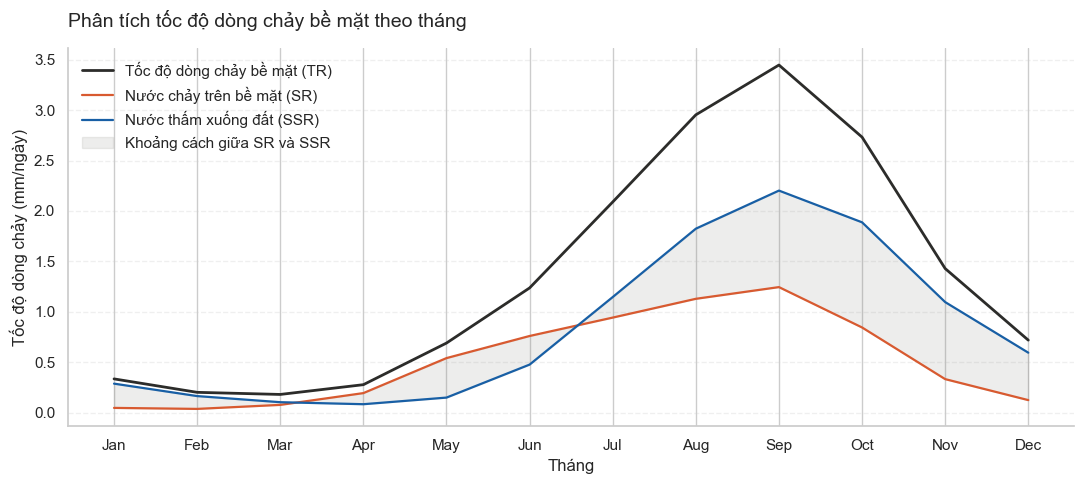
\includegraphics[width=\textwidth]{images/3.8.1.png}
        \caption{Chu kỳ dòng chảy trung bình}
    \end{subfigure}
    \hfill
    \begin{subfigure}[b]{0.48\textwidth}
        \centering
        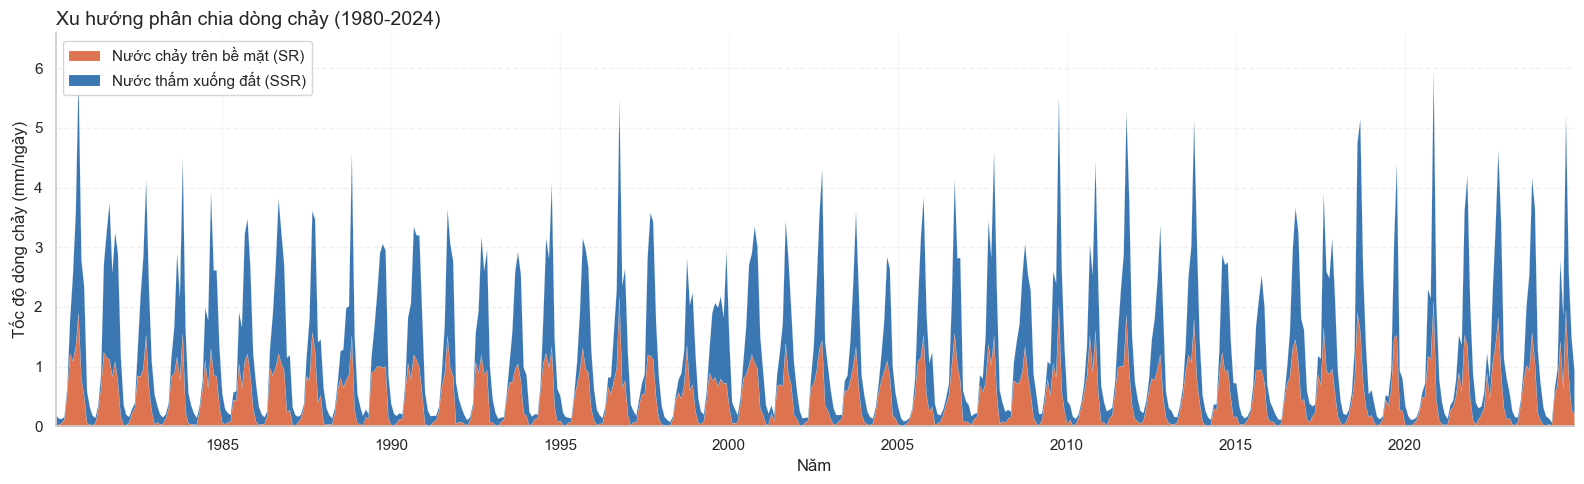
\includegraphics[width=\textwidth]{images/3.8.2.png}
        \caption{Diễn biến phân chia dòng chảy}
    \end{subfigure}
    \caption{Phân tích đặc trưng mùa thủy văn và biến động phân chia nước mặt/ngầm liên năm}
    \label{fig:runoff_cycle_series}
\end{figure}
\FloatBarrier

\subsubsection{Xu hướng lâu dài của tỉ lệ nước bề mặt (SF)}
Dịch chuyển cơ cấu dòng chảy tại \textbf{Hình \ref{fig:runoff_fraction_anomaly}(a)} ghi nhận xu hướng tăng SF hệ thống (+0.00029/năm).

\begin{itemize}
    \item \textbf{Đặc trưng khí hậu (RQ1):} Mặt đệm miền Trung đang giảm dần khả năng hấp thụ tự nhiên và tăng cường xả thẳng nước lên bề mặt sông ngòi. Đặc trưng này cảnh báo sự suy giảm độ ổn định của hệ thống nước ngầm tầng mặt tại khu vực.
    \item \textbf{Tác nhân khắc nghiệt (RQ2):} Biến đổi khí hậu làm gia tăng cường độ mưa tập trung khiến hạ tầng thoát nước quá tải, trực tiếp gây ra các trận lũ lụt thảm khốc hơn. Việc tăng SF đồng nghĩa tác nhân gây lũ bão sẽ tác động nhanh hơn, khốc liệt hơn vào vùng đồng bằng đông dân cư.
\end{itemize}

\subsubsection{Heatmap dị thường tốc độ dòng chảy bề mặt}
Ma trận dị thường tại \textbf{Hình \ref{fig:runoff_fraction_anomaly}(b)} lưu giữ các sự kiện đại hồng thủy lịch sử miền Trung.

\begin{itemize}
    \item \textbf{Đặc trưng khí hậu (RQ1):} Các mảng dị thường dương xanh đậm tập trung cô đặc tháng 9--11, trùng khớp tuyệt đối với cao điểm mùa bão lũ truyền thống. Dòng chảy miền Trung mang đặc trưng biến động cực đại vào cuối năm và cạn kiệt khắc nghiệt vào mùa hè.
    \item \textbf{Tác nhân khắc nghiệt (RQ2):} Dị thường dương xanh đen (tháng 10/1999, 10/2020) phản ánh tác nhân hơi ẩm Biển Đông vượt ngưỡng chịu đựng của thảm thực vật Trường Sơn. Khi mặt đệm bị bão hòa ẩm, mọi lượng mưa thêm vào đều biến thành dòng chảy mặt tàn phá hạ tầng ven sông.
\end{itemize}

\FloatBarrier
\begin{figure}[H]
    \centering
    \begin{subfigure}[b]{0.48\textwidth}
        \centering
        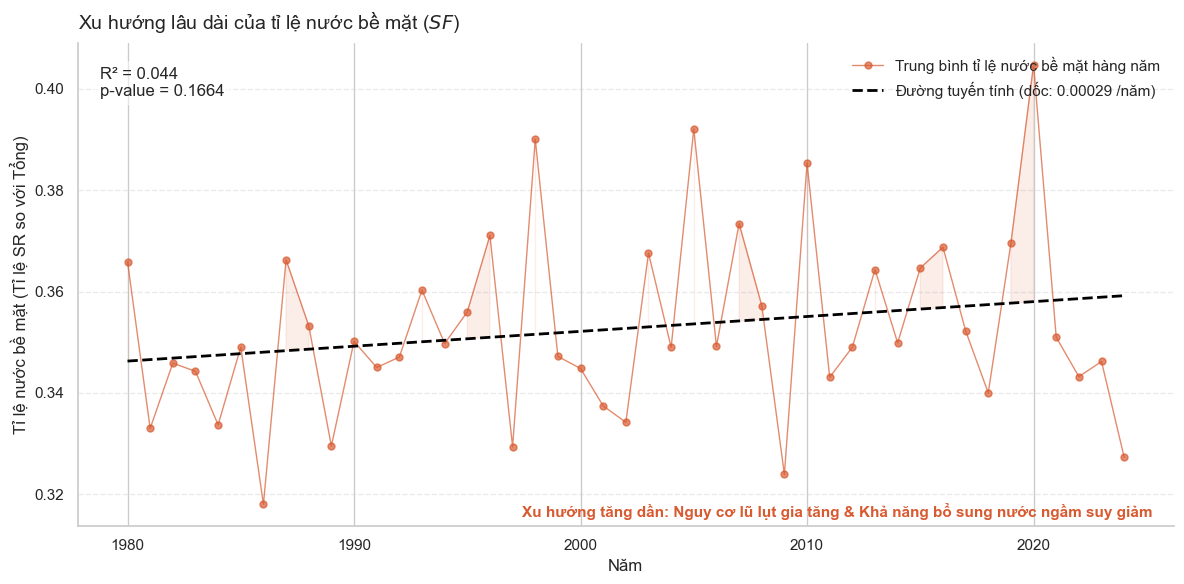
\includegraphics[width=\textwidth]{images/3.8.3.png}
        \caption{Xu hướng tỉ lệ chảy tràn SF}
    \end{subfigure}
    \hfill
    \begin{subfigure}[b]{0.48\textwidth}
        \centering
        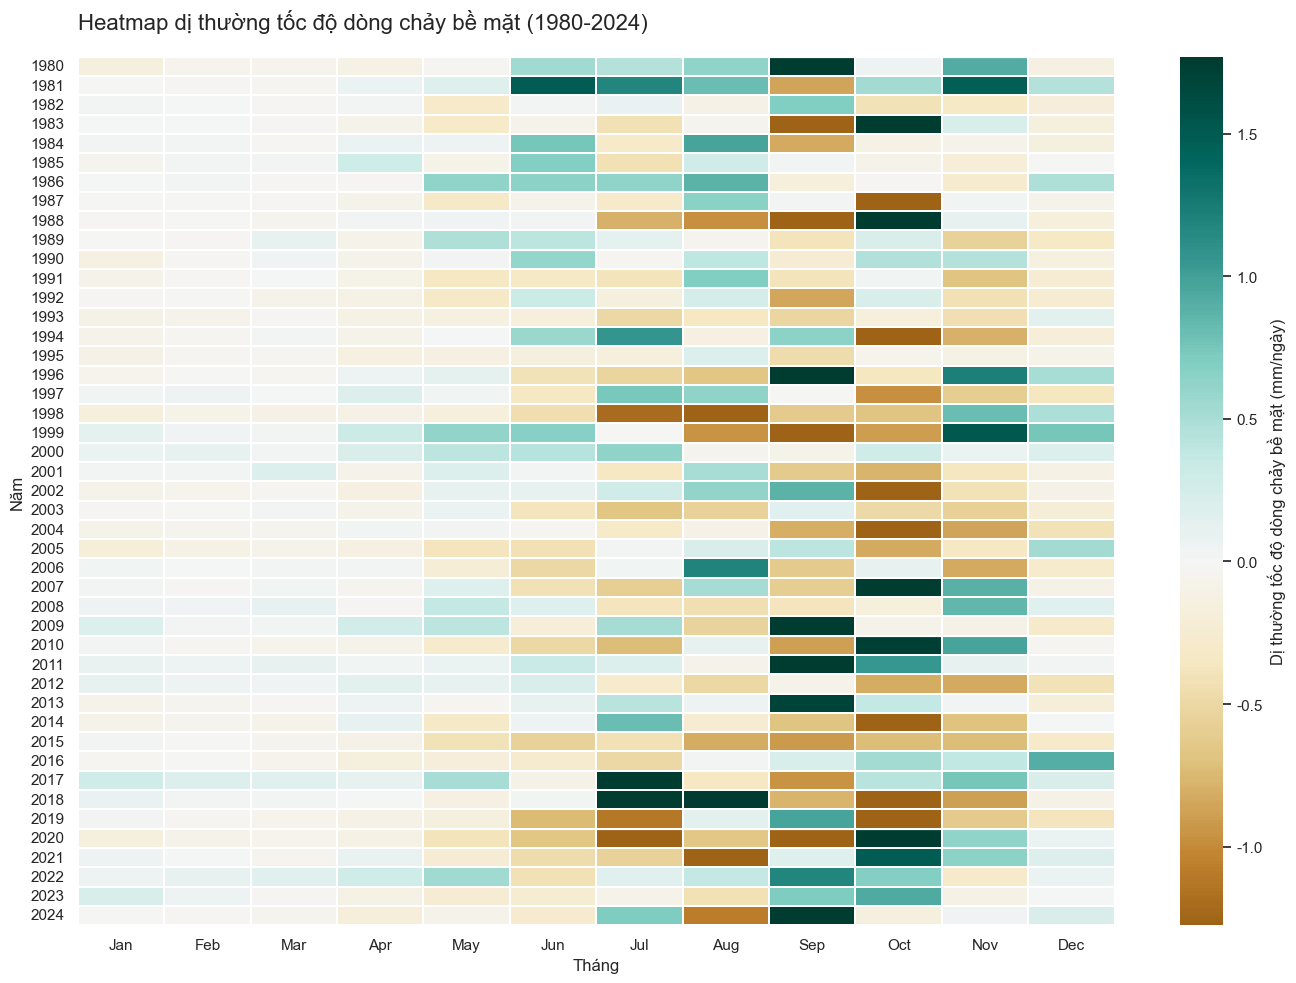
\includegraphics[width=\textwidth]{images/3.8.4.png}
        \caption{Ma trận dị thường dòng chảy mặt}
    \end{subfigure}
    \caption{Phân tích xu hướng cơ cấu xả nước bề mặt và dị thường thủy văn lịch sử}
    \label{fig:runoff_fraction_anomaly}
\end{figure}
\FloatBarrier

\subsubsection{Dấu hiệu tần suất dòng chảy cực đoan}
Số ngày dòng chảy cực đoan (> p95) tại \textbf{Hình \ref{fig:runoff_extreme_days}} cho thấy sự gia tăng tần suất đáng báo động sau mốc 2010.

\begin{itemize}
    \item \textbf{Đặc trưng khí hậu (RQ1):} Miền Trung đang xác lập đặc trưng thiên tai mới: lũ quét và sạt lở xuất hiện thường xuyên và dồn dập hơn qua từng thập kỷ. Sự gia tăng đường trung bình trượt khẳng định tính bất ổn định của chu trình thủy văn khu vực ven biển.
    \item \textbf{Tác nhân khắc nghiệt (RQ2):} Tương tác khốc liệt giữa bão nhiệt đới dồn dập và mặt đệm bão hòa ẩm là tác nhân trực tiếp làm bùng nổ các thảm họa sạt lở đất. Việc số ngày xả nước cực đoan $>25$ ngày/năm vào cuối chuỗi số liệu cảnh báo sự khắc nghiệt ngày càng hung hãn của bão lũ miền Trung.
\end{itemize}

\FloatBarrier
\begin{figure}[H]
    \centering
    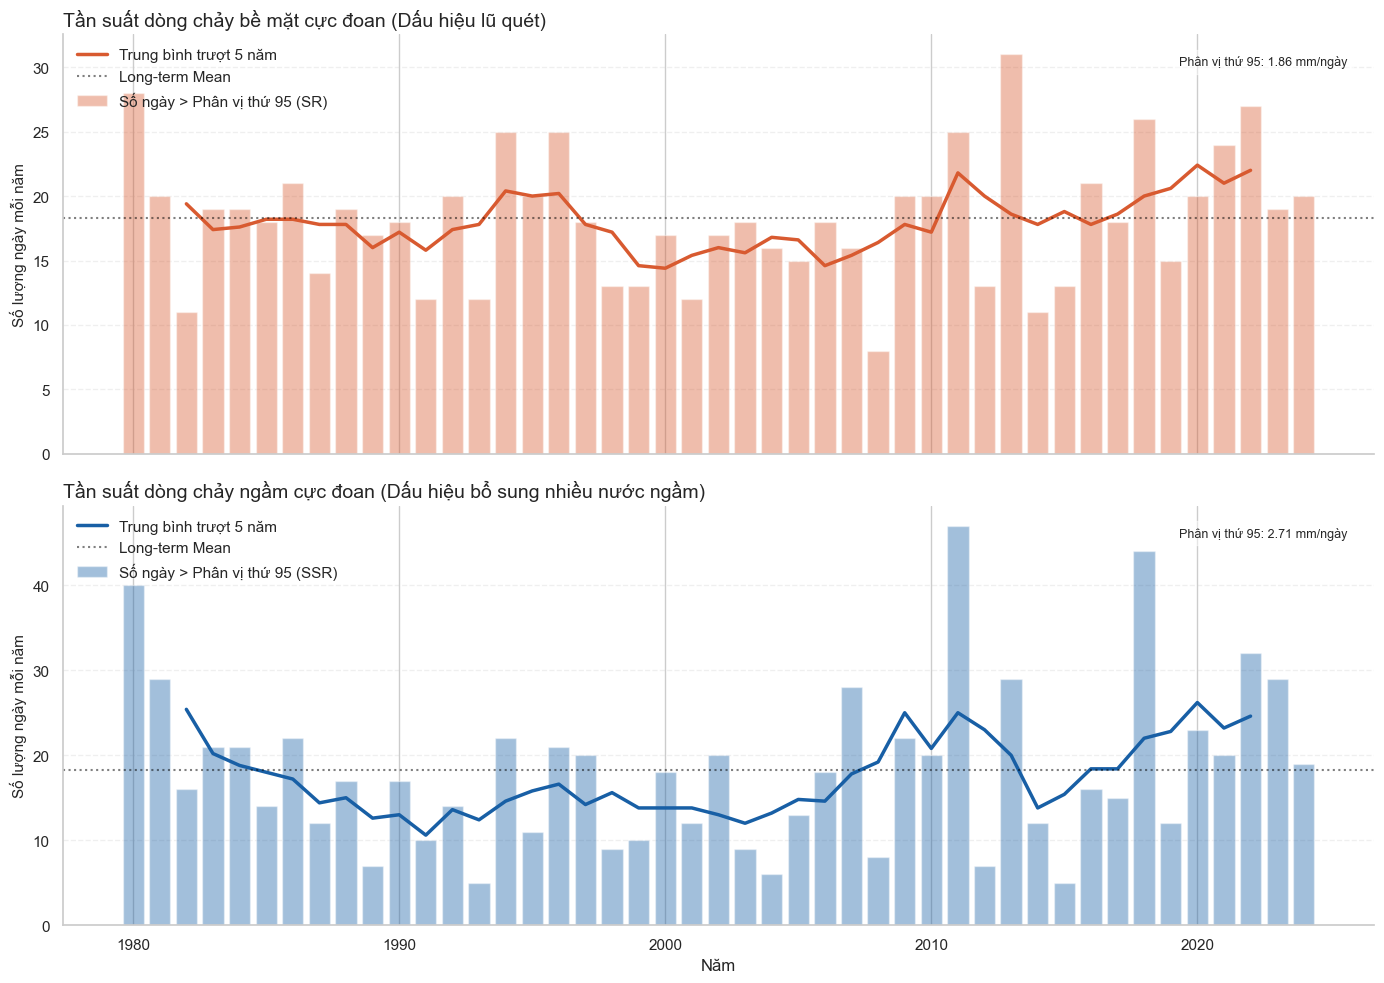
\includegraphics[width=0.7\textwidth]{images/3.8.5.png}
    \caption{Tần suất số ngày có dòng chảy cực đoan (>p95) hàng năm tại miền Trung}
    \label{fig:runoff_extreme_days}
\end{figure}
\FloatBarrier

\subsection{Bức xạ mặt trời}

\subsubsection{Xu hướng bức xạ trung bình năm (Tín hiệu tối đi / sáng lên)}
Biến động năng lượng mặt trời tại bề mặt miền Trung được thể hiện rõ nét qua mô hình hồi quy tại \textbf{Hình \ref{fig:solar_overview}(a)}.

\begin{itemize}
    \item \textbf{Đặc trưng khí hậu (RQ1):} Bức xạ mặt trời tại khu vực duy trì ở nền nhiệt cao, dao động phổ biến từ 175 đến 187.5 $W/m^2$. Giai đoạn 1980--1990 ghi nhận sự tăng trưởng năng lượng (Brightening), tuy nhiên từ sau năm 1991 đến nay, khu vực chuyển sang xu hướng "tối đi" nhẹ.
    \item \textbf{Tác nhân khắc nghiệt (RQ2):} Các đỉnh bức xạ cực đại thường xuất hiện vào những năm khô hạn. Trong các giai đoạn này, \textbf{hiệu ứng phơn} làm tan mây, tạo điều kiện cho năng lượng mặt trời thiêu đốt mặt đệm trực tiếp, đẩy nhiệt độ lên ngưỡng sóng nhiệt cực đoan gây cháy rừng.
\end{itemize}

\subsubsection{Heatmap dị thường trong bức xạ Mặt Trời}
Ma trận tại \textbf{Hình \ref{fig:solar_anomaly_heatmap}} minh chứng cho sự phân cực năng lượng gắt gao giữa hai mùa khí hậu.

\begin{itemize}
    \item \textbf{Đặc trưng khí hậu (RQ1):} Dị thường dương tập trung vào mùa khô từ tháng 3 đến tháng 5, trong khi dị thường âm chiếm ưu thế hoàn toàn vào mùa mưa bão cuối năm. Đặc trưng này xác lập một chu kỳ năng lượng ổn định, chi phối toàn bộ quá trình bốc hơi của thực vật.
    \item \textbf{Tác nhân khắc nghiệt (RQ2):} Các mảng đỏ đậm xuất hiện bất thường gắn liền với sự thống trị của \textbf{vùng áp thấp nóng phía Tây}. Ngược lại, dị thường âm mạnh vào cuối năm là dấu ấn của tác nhân \textbf{Biển Đông} gia tăng mây và các xoáy thuận nhiệt đới.
\end{itemize}

\FloatBarrier
\begin{figure}[H]
    \centering
    \begin{subfigure}[b]{0.48\textwidth}
        \centering
        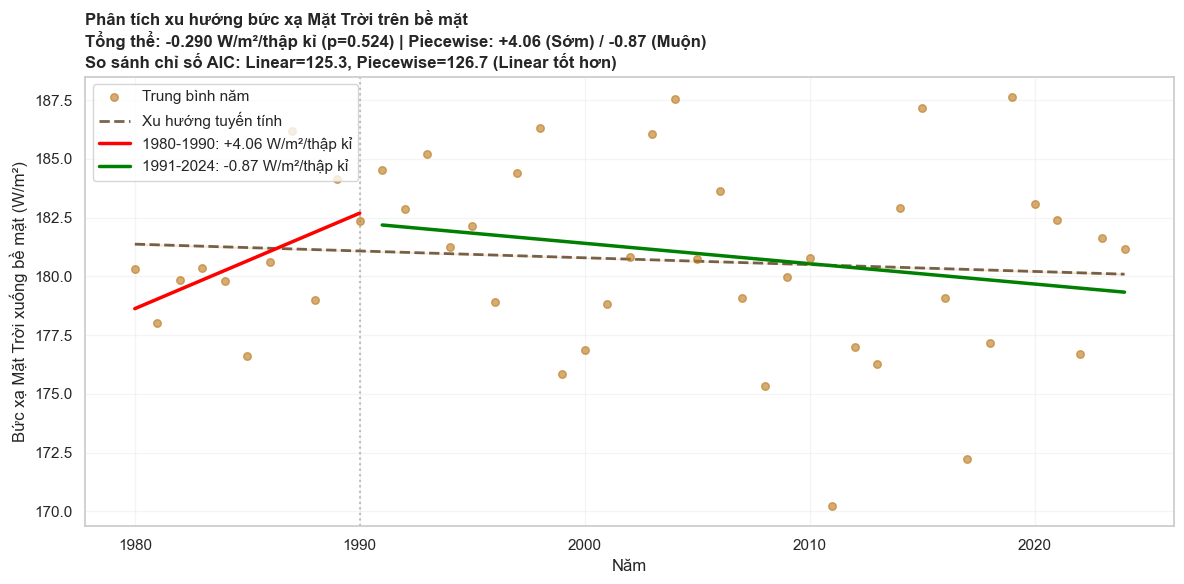
\includegraphics[width=\textwidth]{images/3.9.1.png}
        \caption{Xu hướng biến đổi dài hạn}
    \end{subfigure}
    \hfill
    \begin{subfigure}[b]{0.48\textwidth}
        \centering
        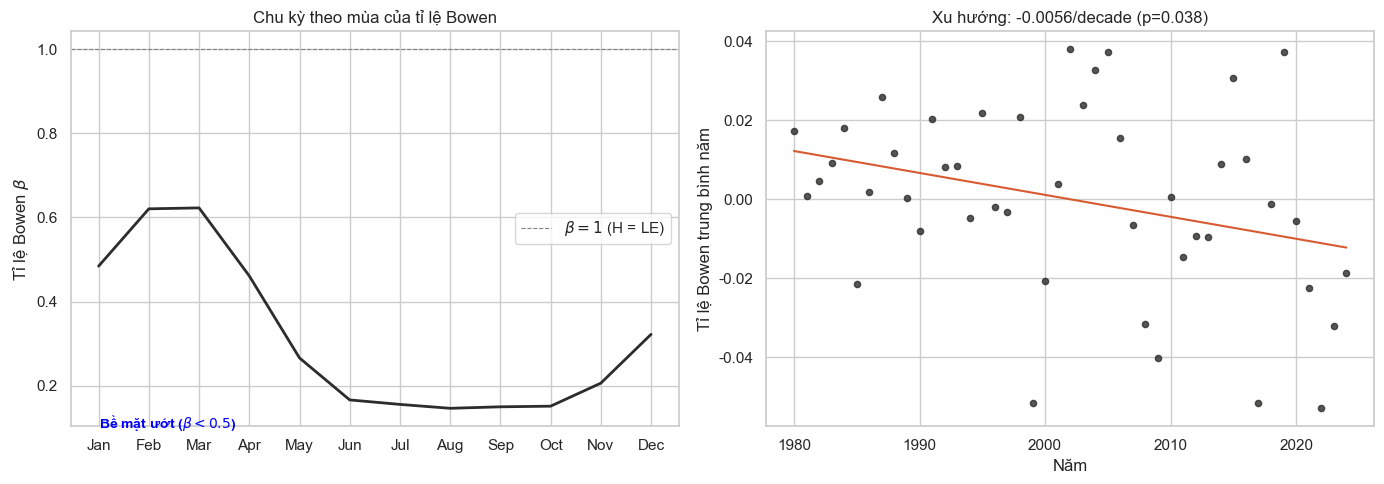
\includegraphics[width=\textwidth]{images/3.10.2.png}
        \caption{Ma trận dị thường hàng tháng}
    \end{subfigure}
    \caption{Phân tích động lực biến đổi bức xạ Mặt Trời và dị thường năng lượng bề mặt}
    \label{fig:solar_overview}
\end{figure}

\begin{figure}[H]
    \centering
    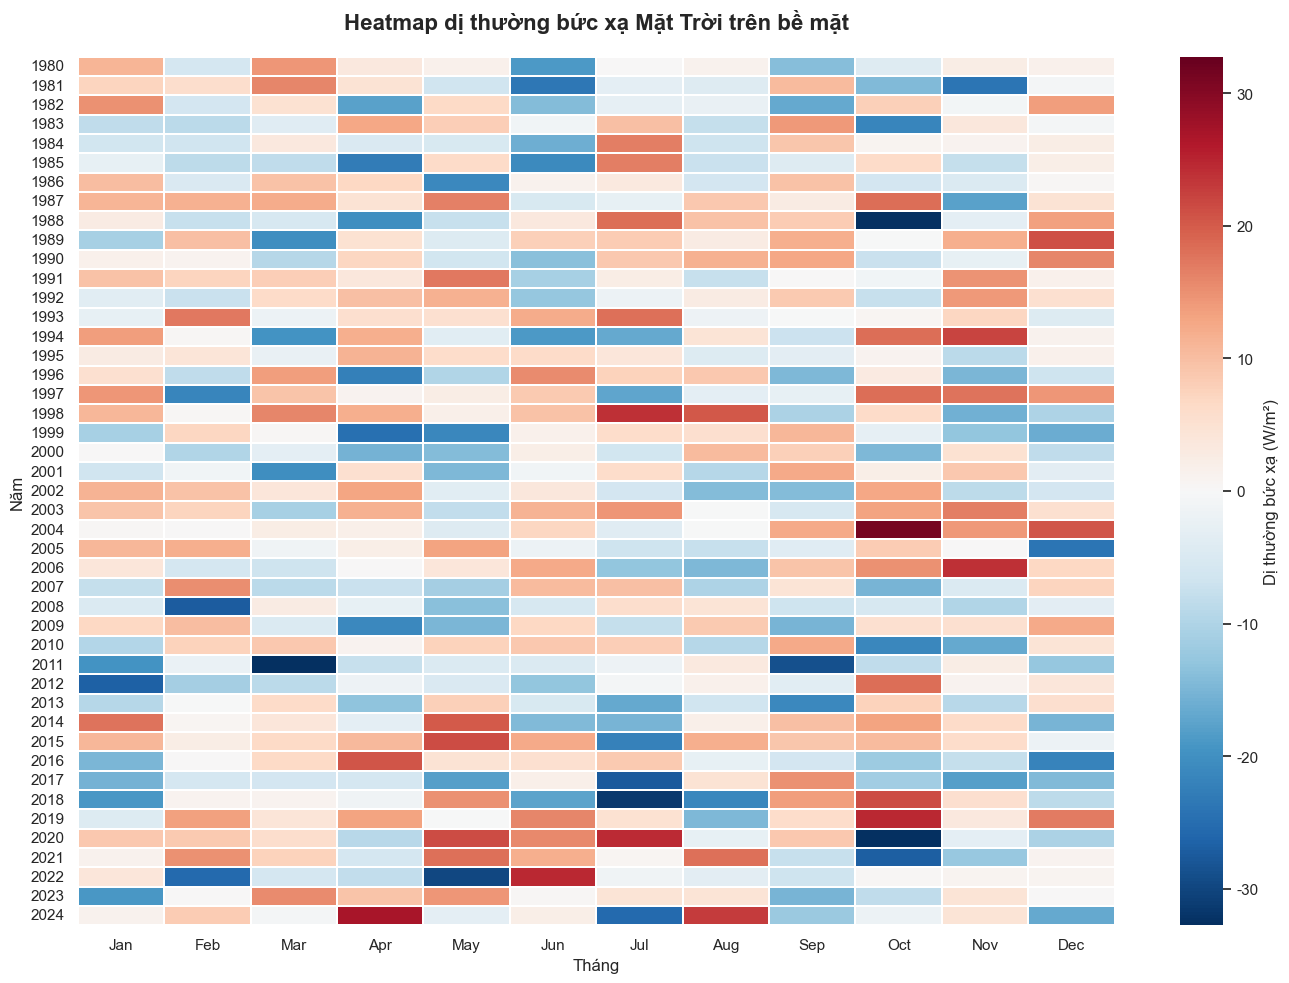
\includegraphics[width=0.7\textwidth]{images/3.9.2.png}
    \caption{Ma trận dị thường bức xạ Mặt Trời hàng tháng (1980--2024)}
    \label{fig:solar_anomaly_heatmap}
\end{figure}
\FloatBarrier

\subsection{Thông lượng nhiệt bề mặt}

\subsubsection{Chu kỳ mùa của hệ năng lượng cân bằng \& Tỉ lệ Bowen}
Cơ cấu phân bổ năng lượng tại bề mặt đệm được trình bày chi tiết tại \textbf{Hình \ref{fig:heat_flux_trends}(a)} và xu hướng tỉ lệ Bowen tại \textbf{Hình \ref{fig:heat_flux_trends}(b)}.

\begin{itemize}
    \item \textbf{Đặc trưng khí hậu (RQ1):} Mặt đệm miền Trung ưu tiên tiêu thụ năng lượng cho nhiệt ẩn ($LE$) để bay hơi hơn là nung nóng khí quyển ($H$), với tỉ lệ Bowen ($\beta$) luôn duy trì dưới ngưỡng 0.5. Đặc trưng "bề mặt đệm ướt" này chi phối toàn bộ cân bằng nhiệt của dải đất ven biển.
    \item \textbf{Tác nhân khắc nghiệt (RQ2):} Việc duy trì nhiệt ẩn cao vào mùa hè là kết quả của luồng hơi ẩm dồi dào từ \textbf{Biển Đông}. Tác nhân này biến miền Trung thành một vùng nóng ẩm oi bức đặc thù, làm gia tăng sự khắc nghiệt đối với sức khỏe con người khi kết hợp nhiệt độ cao.
\end{itemize}

\FloatBarrier
\begin{figure}[H]
    \centering
    \begin{subfigure}[b]{0.48\textwidth}
        \centering
        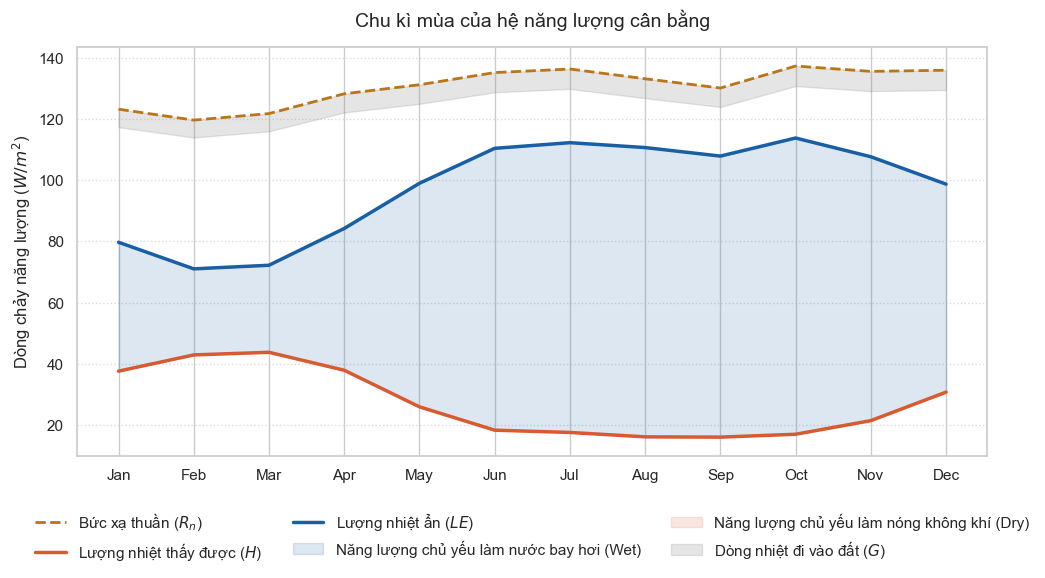
\includegraphics[width=\textwidth]{images/3.10.1.png}
        \caption{Chu kỳ hệ năng lượng cân bằng}
    \end{subfigure}
    \hfill
    \begin{subfigure}[b]{0.48\textwidth}
        \centering
        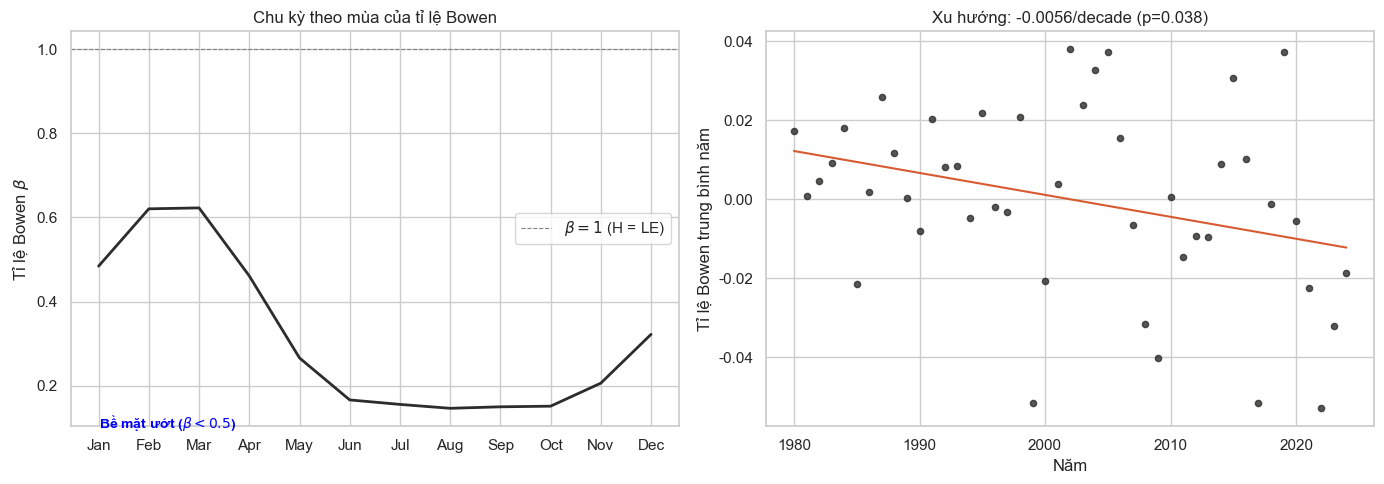
\includegraphics[width=\textwidth]{images/3.10.2.png}
        \caption{Xu hướng tỉ lệ Bowen}
    \end{subfigure}
    \caption{Phân tích đặc trưng tiêu thụ năng lượng mặt đệm và dịch chuyển tỉ lệ nhiệt ẩn}
    \label{fig:heat_flux_trends}
\end{figure}
\FloatBarrier

\subsubsection{Ma trận dị thường tỉ lệ Bowen}
Sự biến động trạng thái năng lượng mặt đệm được thể hiện qua ma trận tại \textbf{Hình \ref{fig:bowen_anomaly_heatmap}}.

\begin{itemize}
    \item \textbf{Đặc trưng khí hậu (RQ1):} Ma trận phản ánh biến động giữa trạng thái khô và ướt; dị thường dương (khô) tập trung nửa đầu năm, dị thường âm (ướt) chiếm ưu thế mùa mưa lũ. Đặc trưng này phản ánh sự nhạy bén của nhiệt độ đất trước chu trình thủy văn.
    \item \textbf{Tác nhân khắc nghiệt (RQ2):} Các mảng đỏ đậm trong năm El Niño minh chứng tác nhân \textbf{gió Lào} triệt tiêu quá trình bay hơi ẩn nhiệt. Tác nhân này đẩy toàn bộ năng lượng vào nhiệt hiện ($H$), khiến nhiệt độ bề mặt tăng vọt và làm trầm trọng hóa hạn hán.
\end{itemize}

\FloatBarrier
\begin{figure}[H]
    \centering
    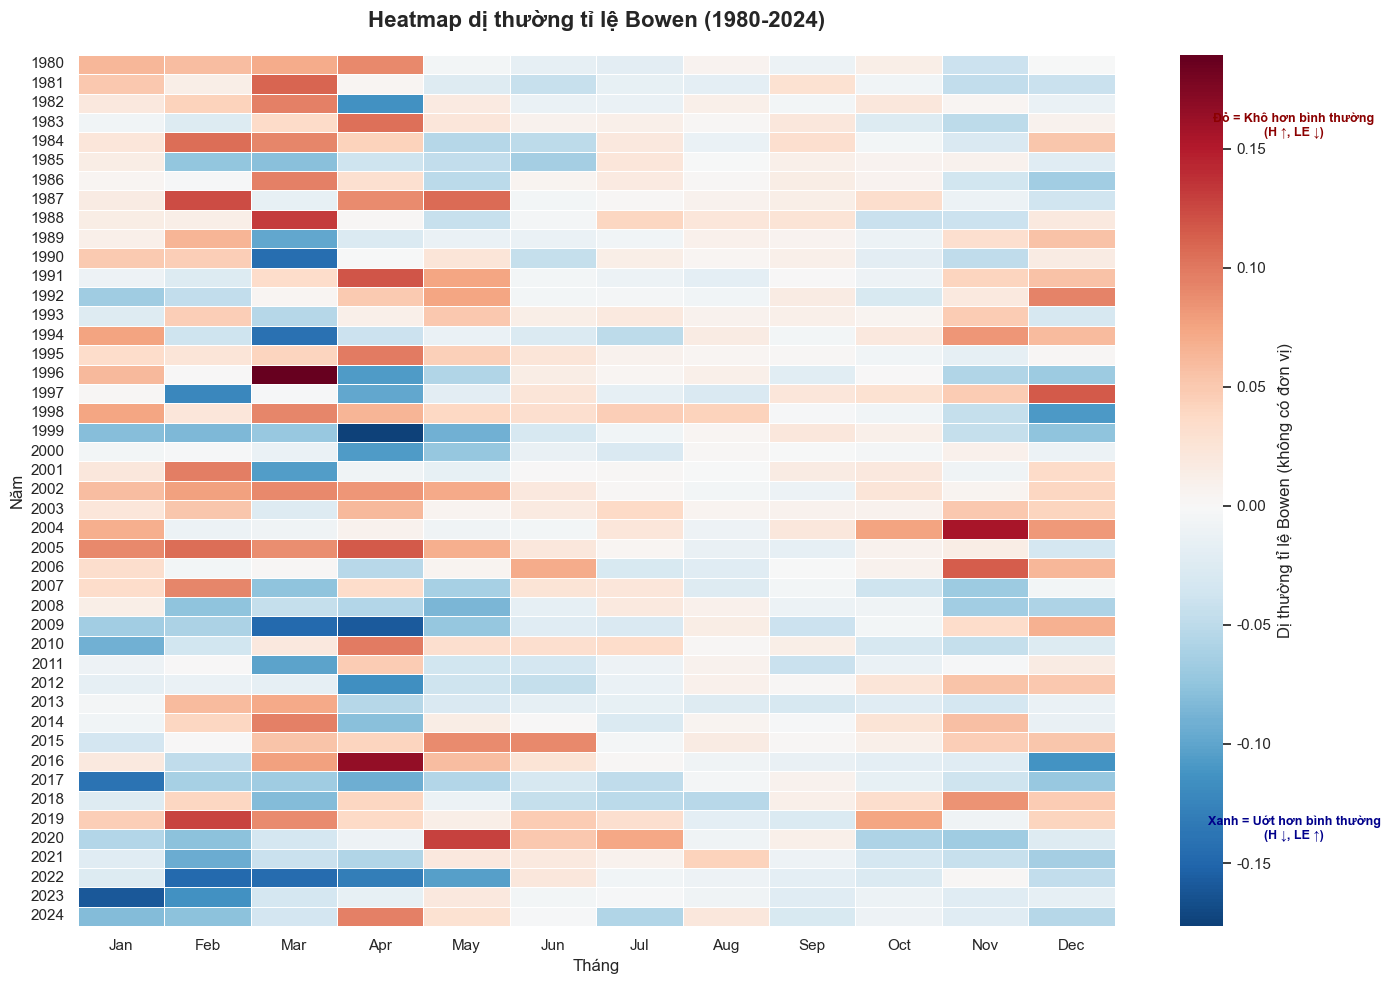
\includegraphics[width=0.7\textwidth]{images/3.10.3.png}
    \caption{Ma trận dị thường tỉ lệ Bowen hàng tháng (1980--2024)}
    \label{fig:bowen_anomaly_heatmap}
\end{figure}
\FloatBarrier

\subsubsection{Xu hướng chuyển dịch tỉ lệ Bowen qua các thập kỷ}
Sự thay đổi phân phối năng lượng theo mùa được trực quan hóa qua biểu đồ hộp tại \textbf{Hình \ref{fig:bowen_decadal}}.

\begin{itemize}
    \item \textbf{Đặc trưng khí hậu (RQ1):} Các hộp boxplot có xu hướng dịch dần xuống phía dưới qua mỗi thập kỷ. Đặc trưng này khẳng định bề mặt miền Trung đang trải qua quá trình ẩm hóa năng lượng hệ thống trong bối cảnh ấm hóa toàn cầu.
    \item \textbf{Tác nhân khắc nghiệt (RQ2):} Sự lấn lướt của nguồn ẩm Biển Đông gây áp lực nhiệt kép. Tác nhân biến đổi khí hậu khiến miền Trung phải đối mặt với trạng thái khắc nghiệt mới: nhiệt độ nền tăng cao nhưng không khí không khô mà lại bão hòa ẩm.
\end{itemize}

\FloatBarrier
\begin{figure}[H]
    \centering
    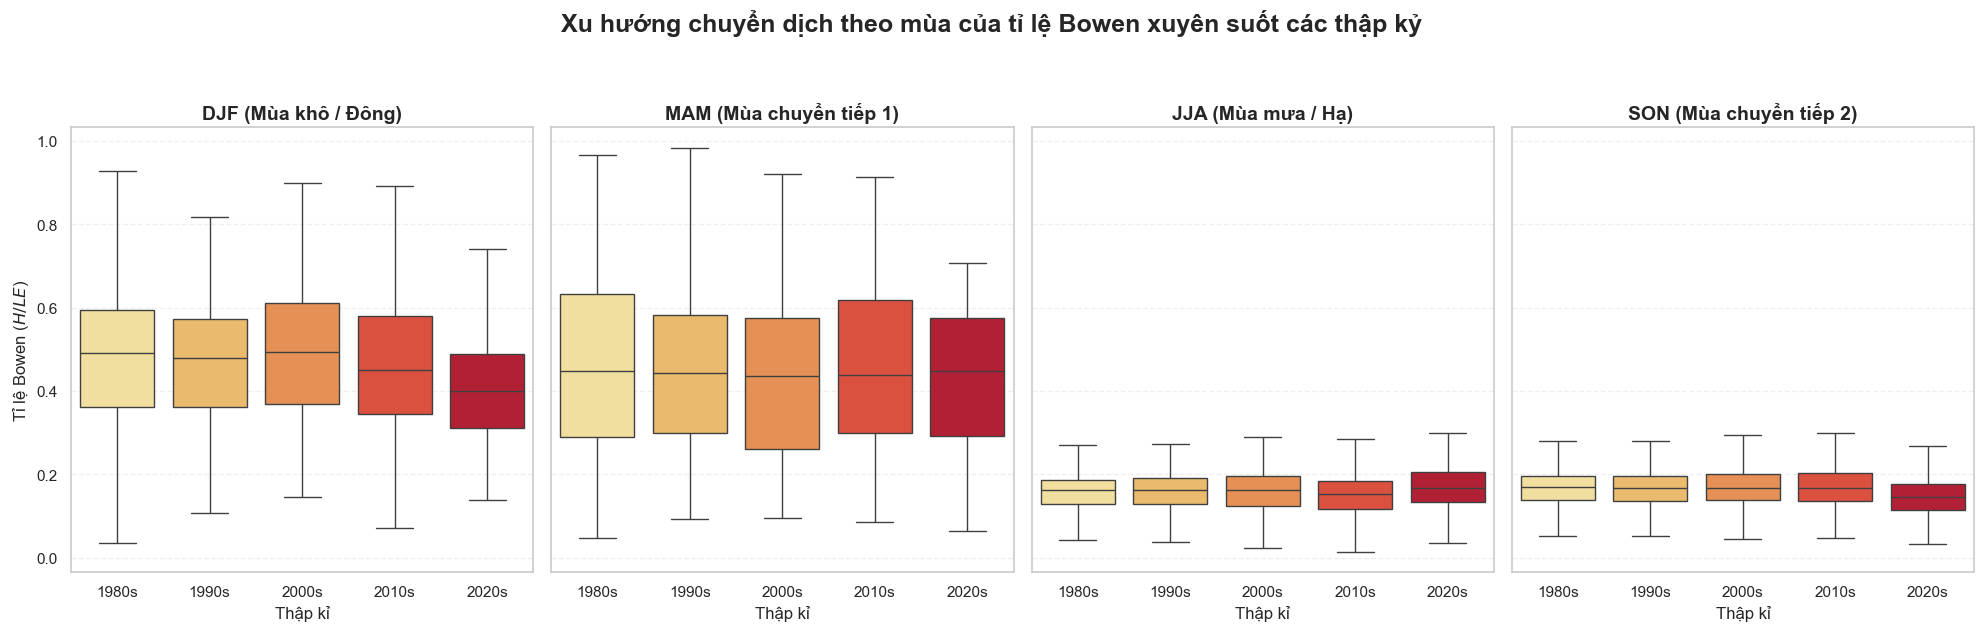
\includegraphics[width=0.7\textwidth]{images/3.10.4.png}
    \caption{Phân phối tỉ lệ Bowen theo các mùa qua từng thập kỷ}
    \label{fig:bowen_decadal}
\end{figure}
\FloatBarrier

\subsection{Cấu trúc thảm thực vật}

\subsubsection{Thành phần lớp phủ bề mặt \& Biến động LAI theo mùa}
Đặc trưng lớp phủ được thể hiện tại \textbf{Hình \ref{fig:veg_overview}(a)} và chu kỳ sinh trưởng diện tích lá tại \textbf{Hình \ref{fig:veg_overview}(b)}.

\begin{itemize}
    \item \textbf{Đặc trưng khí hậu (RQ1):} Lớp phủ miền Trung có sự phân chia cân bằng giữa rừng (33.2%) và đất trống. LAI của rừng luôn duy trì mức vượt trội, đạt đỉnh vào tháng 10--11 bám sát theo chu kỳ mùa mưa lệch muộn đặc thù của khu vực.
    \item \textbf{Tác nhân khắc nghiệt (RQ2):} Sụt giảm LAI vào các tháng 7--8 là minh chứng cho sự "căng thẳng sinh lý" của thực vật dưới tác động của \textbf{gió Lào}. Tác nhân khô nóng này làm suy giảm khả năng phòng hộ của rừng ngay trước thời điểm mùa bão đổ bộ.
\end{itemize}

\FloatBarrier
\begin{figure}[H]
    \centering
    \begin{subfigure}[b]{0.42\textwidth}
        \centering
        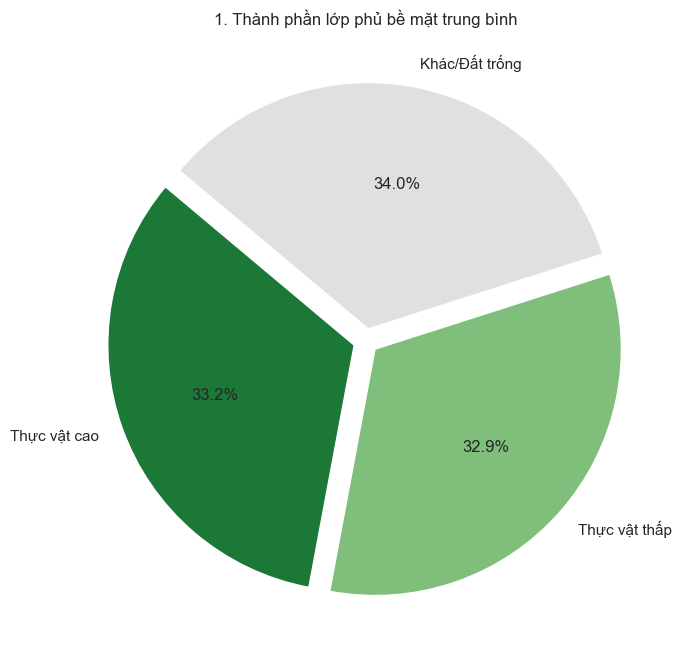
\includegraphics[width=\textwidth]{images/3.11.1.png}
        \caption{Cơ cấu lớp phủ}
    \end{subfigure}
    \hfill
    \begin{subfigure}[b]{0.54\textwidth}
        \centering
        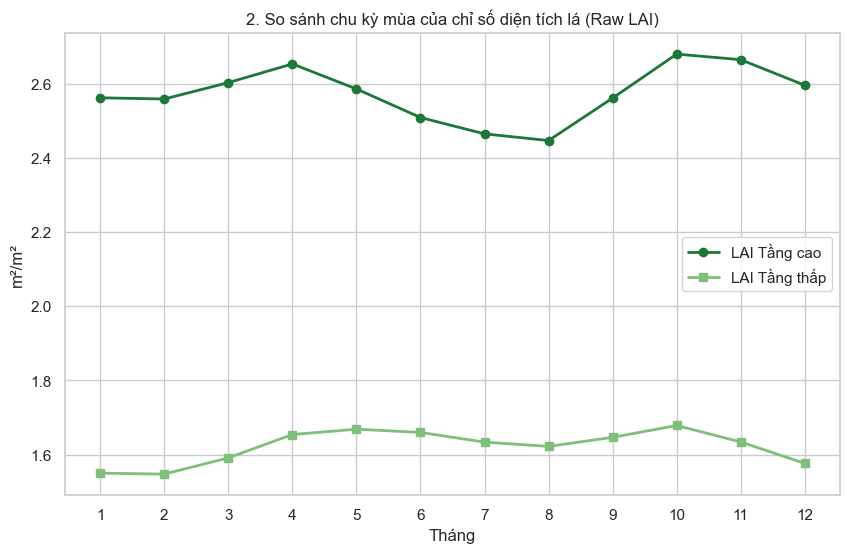
\includegraphics[width=\textwidth]{images/3.11.2.png}
        \caption{Chu kỳ sinh trưởng LAI}
    \end{subfigure}
    \caption{Đặc trưng cấu trúc lớp phủ và động lực thảm xanh thực vật miền Trung}
    \label{fig:veg_overview}
\end{figure}
\FloatBarrier

\subsubsection{Heatmap cường độ xanh của các tầng thực vật}
Ma trận tại \textbf{Hình \ref{fig:veg_greenness}} cho thấy sự ổn định sinh thái khác nhau giữa rừng và cây bụi.

\begin{itemize}
    \item \textbf{Đặc trưng khí hậu (RQ1):} Rừng tầng cao duy trì độ xanh ổn định, khẳng định vai trò điều tiết thủy văn cốt lõi của dãy Trường Sơn. Ngược lại, thực vật thấp biến động mạnh theo thời vụ, phản ánh tính phụ thuộc cao vào chế độ mưa bề mặt.
    \item \textbf{Tác nhân khắc nghiệt (RQ2):} Sự tương phản rõ rệt vào mùa khô phản ánh tính khốc liệt của hạn hán: thực vật thấp suy kiệt nhanh do mất nước mặt đệm. Trong khi đó, rừng tầng cao khai thác nguồn nước ngầm tầng sâu để chống chịu thiêu đốt của bức xạ.
\end{itemize}

\FloatBarrier
\begin{figure}[H]
    \centering
    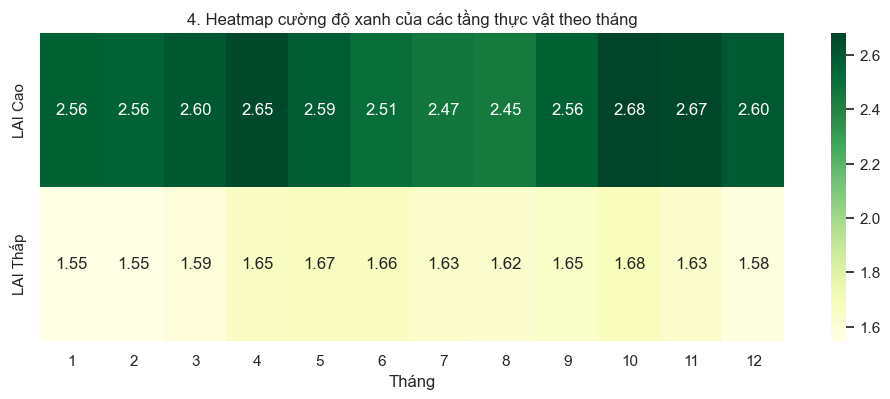
\includegraphics[width=0.7\textwidth]{images/3.11.4.png}
    \caption{Heatmap cường độ xanh của các tầng thực vật theo tháng}
    \label{fig:veg_greenness}
\end{figure}
\FloatBarrier

\subsubsection{Phân tích không gian trạng thái LAI \& Tương quan cấu trúc}
Quỹ đạo sinh trưởng thực vật được thể hiện tại \textbf{Hình \ref{fig:veg_dynamics}(a)} và tương quan tại \textbf{Hình \ref{fig:veg_dynamics}(b)}.

\begin{itemize}
    \item \textbf{Đặc trưng khí hậu (RQ1):} Biểu đồ Phase Plot thể hiện sự thích nghi dài hạn trước chu kỳ bão lũ. Rừng tầng cao luôn đóng vai trò là "mỏ neo" sinh thái ổn định cho khu vực trong mọi thời điểm năm.
    \item \textbf{Tác nhân khắc nghiệt (RQ2):} Tương quan yếu giữa hai tầng thảm phủ minh chứng tác động không đồng nhất: tầng thấp chịu hạn hán mặt đệm, tầng cao gánh chịu lực tàn phá của gió bão từ \textbf{Biển Đông}. Tác nhân bão làm gãy đổ cây tầng cao, gây thiệt hại rừng phòng hộ.
\end{itemize}

\FloatBarrier
\begin{figure}[H]
    \centering
    \begin{subfigure}[b]{0.48\textwidth}
        \centering
        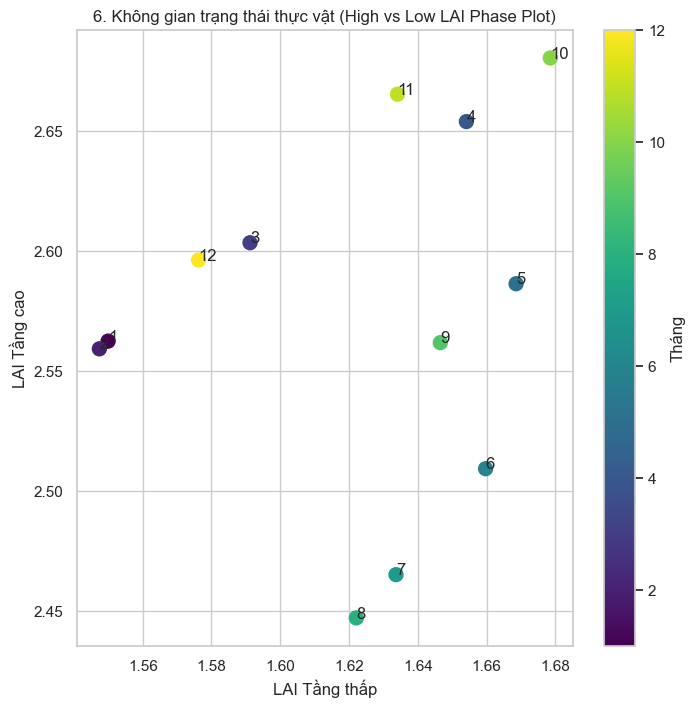
\includegraphics[width=\textwidth]{images/3.11.6.png}
        \caption{Không gian trạng thái thực vật}
    \end{subfigure}
    \hfill
    \begin{subfigure}[b]{0.48\textwidth}
        \centering
        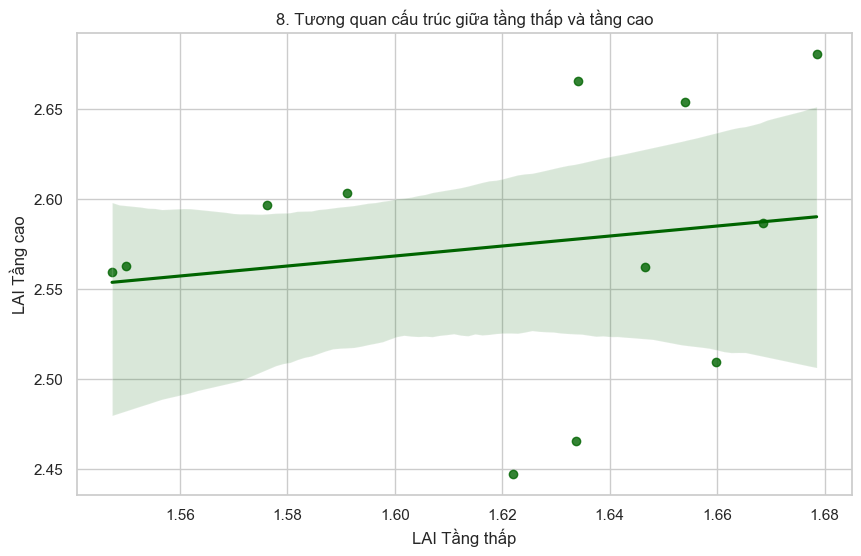
\includegraphics[width=\textwidth]{images/3.11.7.png}
        \caption{Tương quan High vs Low LAI}
    \end{subfigure}
    \caption{Phân tích mối quan hệ động lực và độ ổn định của các tầng thực vật}
    \label{fig:veg_dynamics}
\end{figure}
\FloatBarrier

\subsection{Độ che phủ mây}

\subsubsection{Khí hậu học độ che phủ mây: Tổng lượng mây vs Mây các tầng}
Cấu trúc phân tầng mây được trình bày tại \textbf{Hình \ref{fig:cloud_climatology}}.

\begin{itemize}
    \item \textbf{Đặc trưng khí hậu (RQ1):} Tổng lượng mây miền Trung duy trì ở ngưỡng cao, thống trị bởi mây tầng cao (HCC). Khu vực mang đặc trưng khí hậu "hiếm khi quang đãng" với số ngày u ám chiếm ưu thế, xác lập trạng thái bầu trời ít ánh sáng trực tiếp.
    \item \textbf{Tác nhân khắc nghiệt (RQ2):} Mây HCC mùa hè từ dải hội tụ \textbf{ITCZ}. Trong khi đó, mây LCC mùa đông do \textbf{gió mùa Đông Bắc} bị chặn bởi \textbf{Trường Sơn}, tạo đặc trưng u ám rét ẩm kéo dài khốc liệt cho khu vực ven biển.
\end{itemize}

\FloatBarrier
\begin{figure}[H]
    \centering
    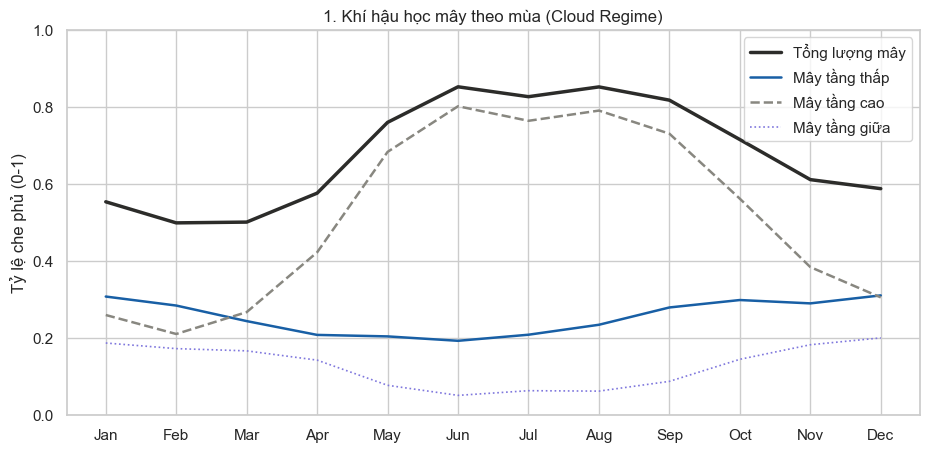
\includegraphics[width=0.7\textwidth]{images/3.12.1.png}
    \caption{Chu kỳ mùa trung bình của tổng lượng mây và mây các tầng}
    \label{fig:cloud_climatology}
\end{figure}
\FloatBarrier

\subsubsection{Chu kỳ mùa và xu hướng của chỉ số thống trị (LCC-HCC)}
Biến động chỉ số thống trị mây tại \textbf{Hình \ref{fig:cloud_trends}(a)} cho thấy sự dịch chuyển vật lý hệ thống.

\begin{itemize}
    \item \textbf{Đặc trưng khí hậu (RQ1):} Chỉ số thống trị âm khẳng định bầu trời miền Trung mang đặc tính mây đối lưu sâu. Xu hướng này duy trì ổn định, xác lập một cấu trúc tầng mây đặc thù của dải đất ven biển.
    \item \textbf{Tác nhân khắc nghiệt (RQ2):} Xu hướng giảm mạnh chỉ số thống trị xác nhận \textbf{gia tăng bất ổn định khí quyển}. Việc HCC ngày càng áp đảo LCC báo hiệu sự bùng nổ của các đám mây dông mạnh, gia tăng thiên tai giông sét nguy hiểm.
\end{itemize}

\subsubsection{Ma trận dị thường tổng lượng mây hàng tháng}
Biến động mây lịch sử được trực quan hóa tại \textbf{Hình \ref{fig:cloud_anomaly_heatmap}}.

\begin{itemize}
    \item \textbf{Đặc trưng khí hậu (RQ1):} Ma trận phản ánh các chu kỳ ít mây kỷ lục gắn chặt với pha El Niño. Ngược lại, dư thừa mây vào các năm La Niña gây tình trạng thiếu hụt ánh sáng kéo dài cho các hoạt động sản xuất nông nghiệp.
    \item \textbf{Tác nhân khắc nghiệt (RQ2):} Các năm ít mây đột biến chính là thời điểm \textbf{hiệu ứng phơn} khốc liệt nhất, cho phép bức xạ Mặt Trời thiêu đốt mặt đệm mà không được che chắn, bùng phát cháy rừng Trường Sơn.
\end{itemize}

\FloatBarrier
\begin{figure}[H]
    \centering
    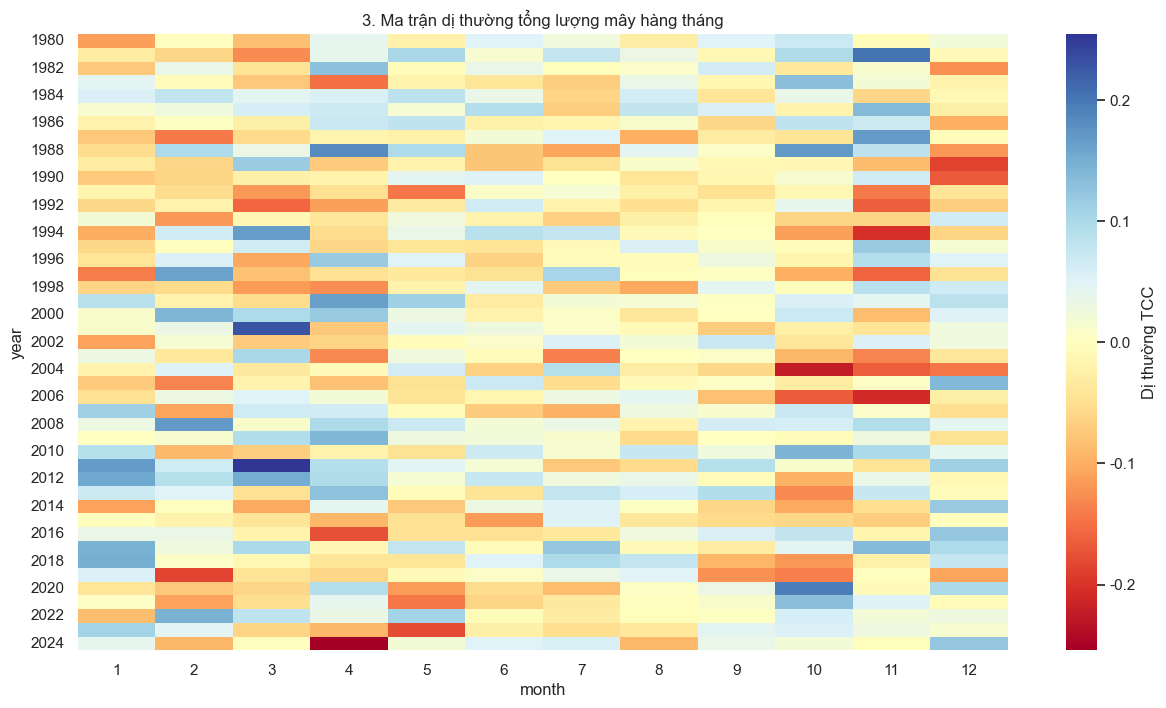
\includegraphics[width=0.7\textwidth]{images/3.12.3.png}
    \caption{Ma trận dị thường tổng lượng mây hàng tháng (1980--2024)}
    \label{fig:cloud_anomaly_heatmap}
\end{figure}

\begin{figure}[H]
    \centering
    \begin{subfigure}[b]{0.48\textwidth}
        \centering
        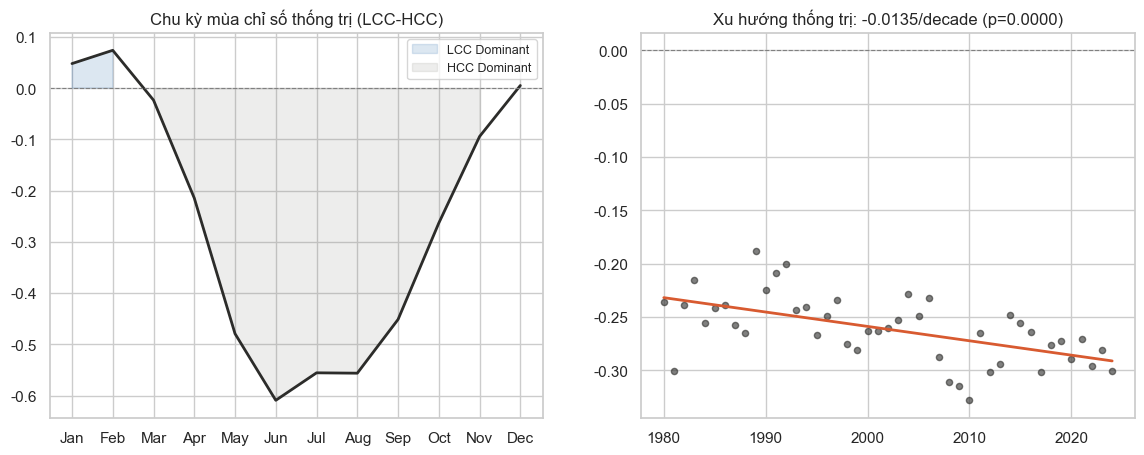
\includegraphics[width=\textwidth]{images/3.12.2.png}
        \caption{Chu kỳ và xu hướng thống trị}
    \end{subfigure}
    \hfill
    \begin{subfigure}[b]{0.48\textwidth}
        \centering
        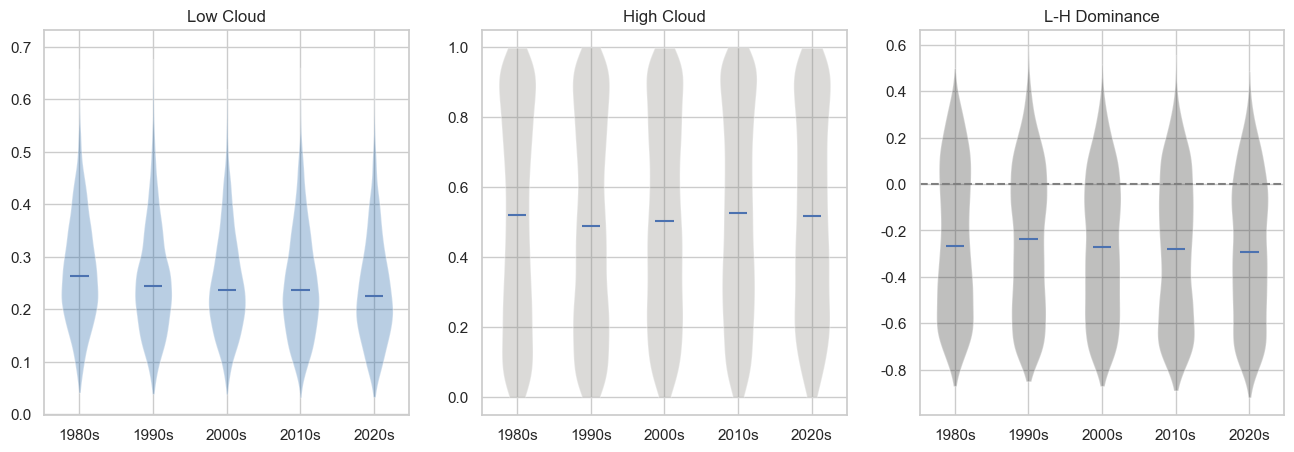
\includegraphics[width=\textwidth]{images/3.12.6.png}
        \caption{Phân phối cấu trúc mây}
    \end{subfigure}
    \caption{Phân tích xu hướng chỉ số thống trị mây và dịch chuyển phân phối theo thập kỷ}
    \label{fig:cloud_trends}
\end{figure}
\FloatBarrier

\subsection{Bất ổn định đối lưu}

\subsubsection{Khí hậu học chỉ số CAPE và các chỉ số bất ổn định}
Chu kỳ tiềm năng đối lưu được thể hiện tại \textbf{Hình \ref{fig:conv_overview}(a)} và động lực ngày đêm tại \textbf{Hình \ref{fig:conv_overview}(b)}.

\begin{itemize}
    \item \textbf{Đặc trưng khí hậu (RQ1):} Các chỉ số đối lưu đạt cực đại vào tháng 6, tích lũy năng lượng tiềm tàng mạnh nhất. CAPE mang đặc trưng ngày đêm vô cùng mạnh mẽ, thường đạt đỉnh cực đại vào lúc 19:00 giờ địa phương.
    \item \textbf{Tác nhân khắc nghiệt (RQ2):} Đỉnh chiều tối là hệ quả của tích lũy nhiệt suốt ngày kết hợp gió từ \textbf{Biển Đông} thổi vào. Cơ chế này lý giải tại sao các trận dông lốc thường kích phát đột ngột vào lúc chạng vạng, gây khó khăn cho phòng tránh.
\end{itemize}

\FloatBarrier
\begin{figure}[H]
    \centering
    \begin{subfigure}[b]{0.48\textwidth}
        \centering
        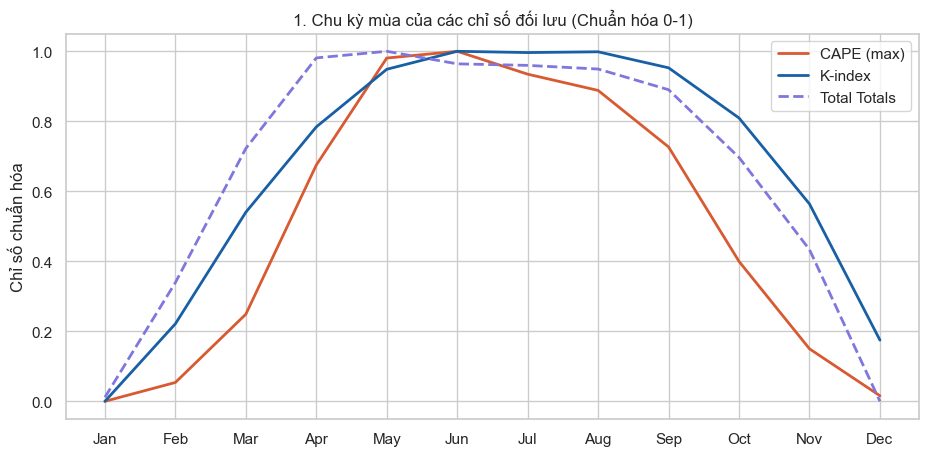
\includegraphics[width=\textwidth]{images/3.13.1.png}
        \caption{Chu kỳ mùa các chỉ số}
    \end{subfigure}
    \hfill
    \begin{subfigure}[b]{0.48\textwidth}
        \centering
        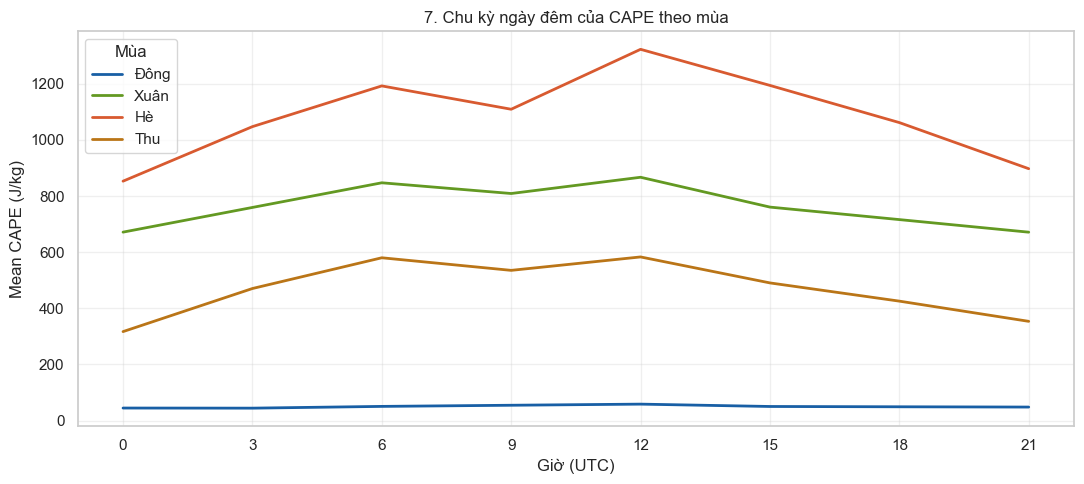
\includegraphics[width=\textwidth]{images/3.13.6.png}
        \caption{Chu kỳ ngày đêm của CAPE}
    \end{subfigure}
    \caption{Phân tích đặc trưng tích lũy năng lượng đối lưu và động lực ngày đêm theo mùa}
    \label{fig:conv_overview}
\end{figure}
\FloatBarrier

\subsubsection{Ma trận dị thường chỉ số đối lưu tổng hợp (CII)}
Biến động giông bão lịch sử được trình bày tại \textbf{Hình \ref{fig:cii_anomaly_heatmap}}.

\begin{itemize}
    \item \textbf{Đặc trưng khí hậu (RQ1):} Ma trận CII cho thấy "mùa giông bão" có xu hướng mở rộng sang các tháng chuyển tiếp đầu hè và cuối thu. Đặc trưng này xác lập dải thời gian nguy hiểm kéo dài cho các hoạt động ngoài trời tại miền Trung.
    \item \textbf{Tác nhân khắc nghiệt (RQ2):} Dị thường dương tập trung mạnh vào các năm nắng nóng kỷ lục do nhiệt độ nền tăng cao kích hoạt bất ổn định cực độ. Tác nhân này khiến miền Trung hứng chịu thời tiết nguy hiểm ngay sau mỗi đợt sóng nhiệt.
\end{itemize}

\FloatBarrier
\begin{figure}[H]
    \centering
    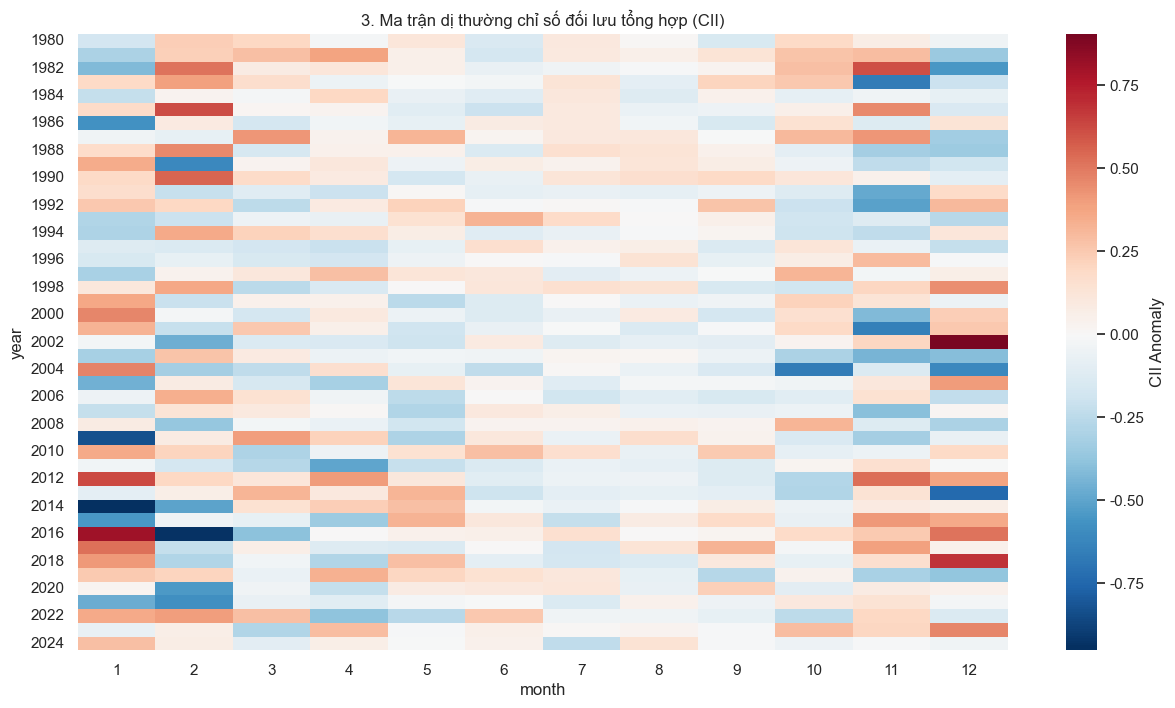
\includegraphics[width=0.7\textwidth]{images/3.13.3.png}
    \caption{Ma trận dị thường chỉ số đối lưu tổng hợp (CII) hàng tháng}
    \label{fig:cii_anomaly_heatmap}
\end{figure}
\FloatBarrier

\subsubsection{Xu hướng của các trị số CAPE cực đoan}
Sự thay đổi cấu trúc năng lượng được minh chứng qua xu hướng tại \textbf{Hình \ref{fig:conv_extremes}}.

\begin{itemize}
    \item \textbf{Đặc trưng khí hậu (RQ1):} Mặc dù năng lượng trung bình giảm nhẹ, các trị số cực hạn (p99) lại tăng mạnh (+24.3 J/kg/thập kỷ). Đặc trưng này cho thấy sự dồn nén năng lượng vào các sự kiện hiếm gặp có sức tàn phá khổng lồ.
    \item \textbf{Tác nhân khắc nghiệt (RQ2):} Gia tăng p99 báo hiệu tương lai \textbf{cực đoan hóa khí hậu}: dông bão trở nên hung hãn và dữ dội hơn gấp bội. Tác nhân này trực tiếp làm gia tăng cường độ giông lốc và cuồng phong tại khu vực.
\end{itemize}

\FloatBarrier
\begin{figure}[H]
    \centering
    \begin{subfigure}[b]{0.48\textwidth}
        \centering
        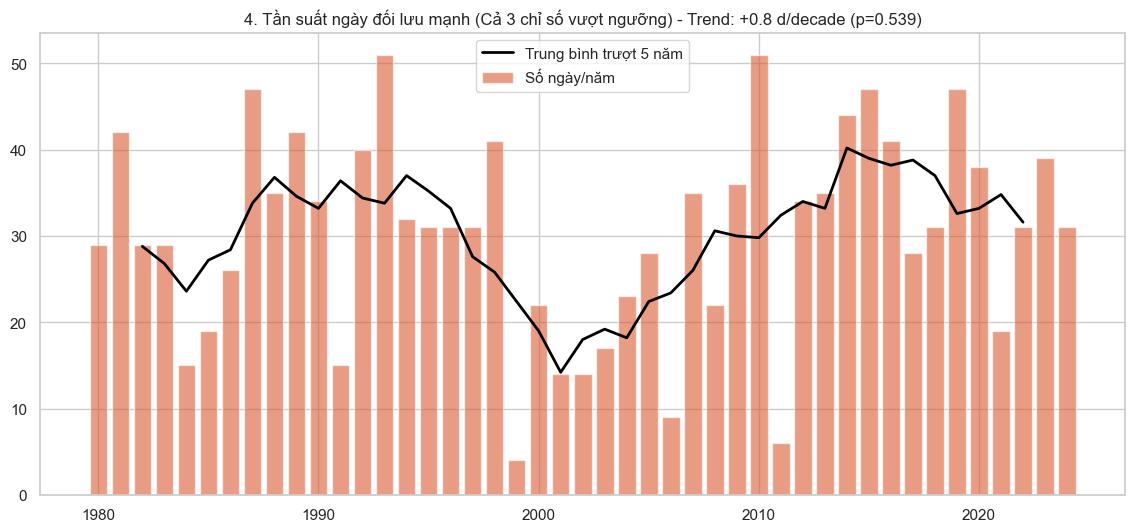
\includegraphics[width=\textwidth]{images/3.13.4.png}
        \caption{Số ngày đối lưu mạnh}
    \end{subfigure}
    \hfill
    \begin{subfigure}[b]{0.48\textwidth}
        \centering
        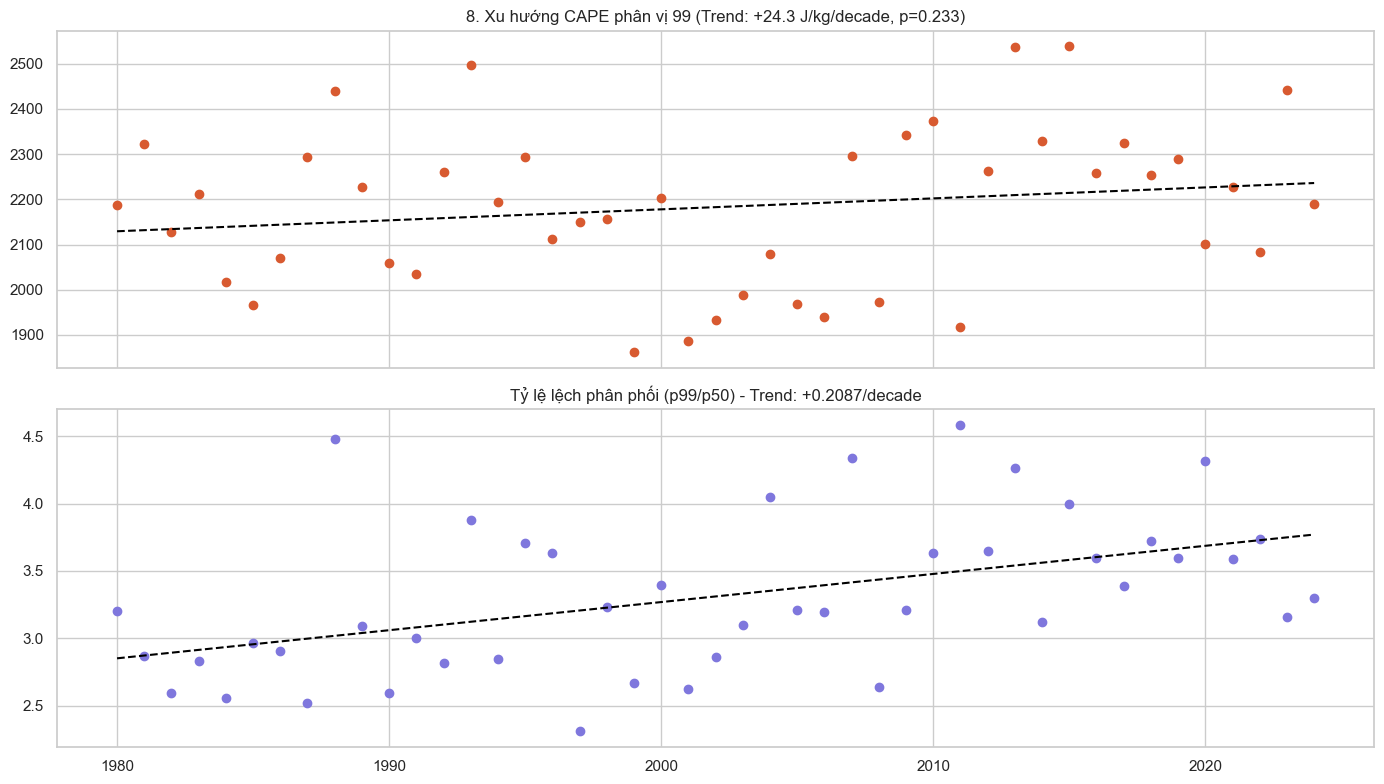
\includegraphics[width=\textwidth]{images/3.13.7.png}
        \caption{Xu hướng CAPE cực đoan (p99)}
    \end{subfigure}
    \caption{Phân tích tần suất giông bão và xu hướng cực đoan hóa năng lượng ẩm khí quyển}
    \label{fig:conv_extremes}
\end{figure}
\FloatBarrier

\subsection{Gió}

\subsubsection{Đặc điểm trường gió bề mặt (10m) và tầng cao (100m)}
Đặc trưng gió theo mùa được thể hiện rõ nét qua biểu đồ hoa gió tại \textbf{Hình \ref{fig:wind_climatology_roses}}.

\begin{itemize}
    \item \textbf{Đặc trưng khí hậu (RQ1):} Miền Trung thể hiện sự đảo chiều gió mùa rõ rệt: gió Đông Bắc (NE) vào mùa Đông và gió Tây Nam (SW) vào mùa Hạ. Tốc độ gió tại 100m luôn vượt trội và có độ tập trung hướng cao hơn so với tầng sát bề mặt.
    \item \textbf{Tác nhân khắc nghiệt (RQ2):} Khác nghiệt thể hiện qua \textbf{gió mùa Đông Bắc} mạnh mang khí lạnh tràn sâu xuống phía Nam. Ngược lại, luồng gió Tây Nam vượt qua \textbf{dãy Trường Sơn} tạo hiệu ứng phơn khô nóng, gây hạn hán và cháy rừng.
\end{itemize}

\FloatBarrier
\begin{figure}[H]
    \centering
    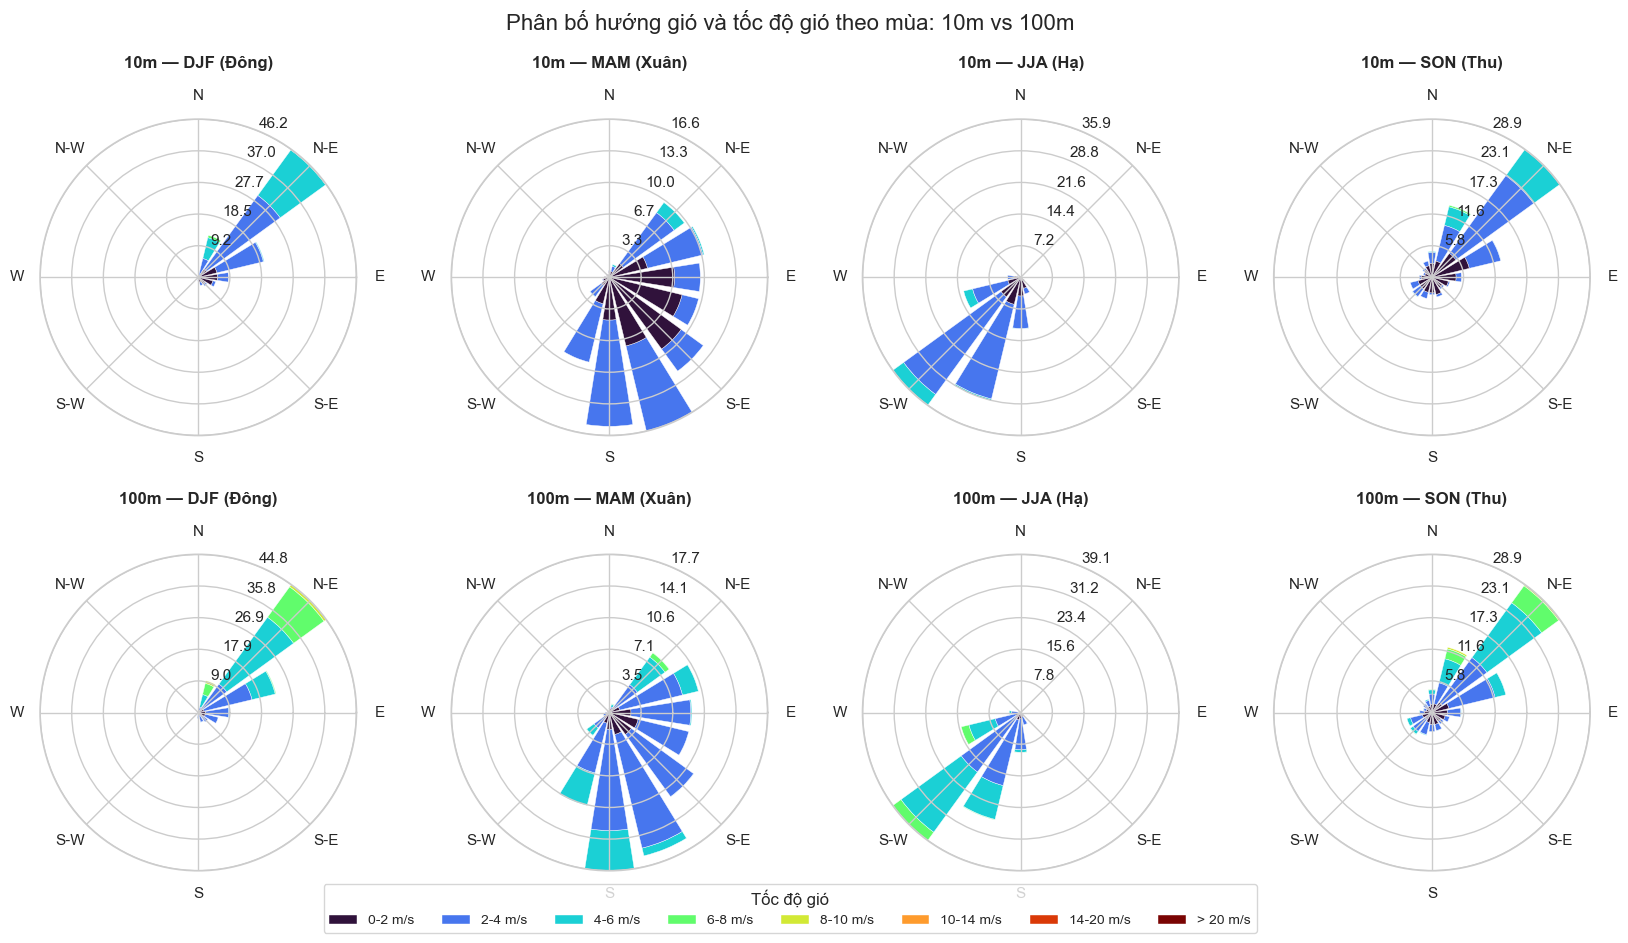
\includegraphics[width=0.85\textwidth]{images/3.14.1.png}
    \caption{Hoa gió phân bổ hướng và tốc độ gió theo mùa tại độ cao 10m và 100m}
    \label{fig:wind_climatology_roses}
\end{figure}
\FloatBarrier

\subsubsection{Biến động tốc độ gió theo mùa \& Xu hướng dài hạn của tốc độ gió}
Chu kỳ mùa tại \textbf{Hình \ref{fig:wind_speed_overview}(a)} và xu hướng năm tại \textbf{Hình \ref{fig:wind_speed_overview}(b)}.

\begin{itemize}
    \item \textbf{Đặc trưng khí hậu (RQ1):} Tốc độ gió có hai đỉnh: đỉnh chính tháng 12--1 và đỉnh phụ tháng 6--7. Về dài hạn, tốc độ gió trung bình duy trì sự ổn định đáng kinh ngạc trong suốt 45 năm qua với xu hướng biến đổi cực nhỏ.
    \item \textbf{Tác nhân khắc nghiệt (RQ2):} Khoảng cách tốc độ 10m và 100m nới rộng nhất vào mùa hè, minh chứng nung nóng bề mặt gia tăng đứt gãy gió. Tác nhân \textbf{không khí lạnh tăng cường} thường tạo ra các luồng xiết lạnh mạnh ở tầng cao.
\end{itemize}

\FloatBarrier
\begin{figure}[H]
    \centering
    \begin{subfigure}[b]{0.48\textwidth}
        \centering
        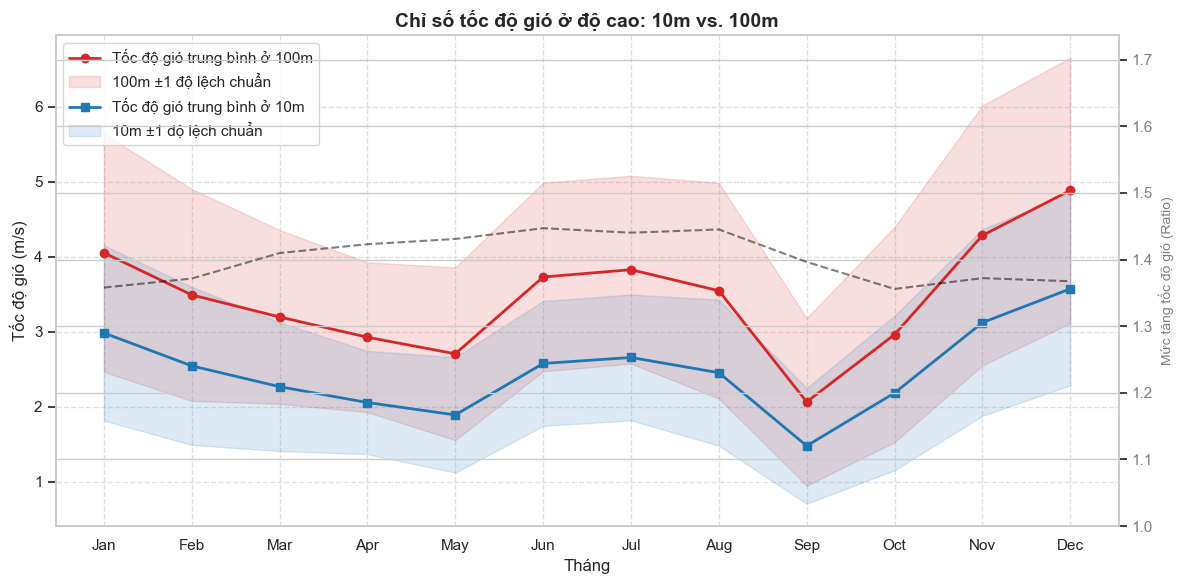
\includegraphics[width=\textwidth]{images/3.14.2.png}
        \caption{Chu kỳ mùa tốc độ gió}
    \end{subfigure}
    \hfill
    \begin{subfigure}[b]{0.48\textwidth}
        \centering
        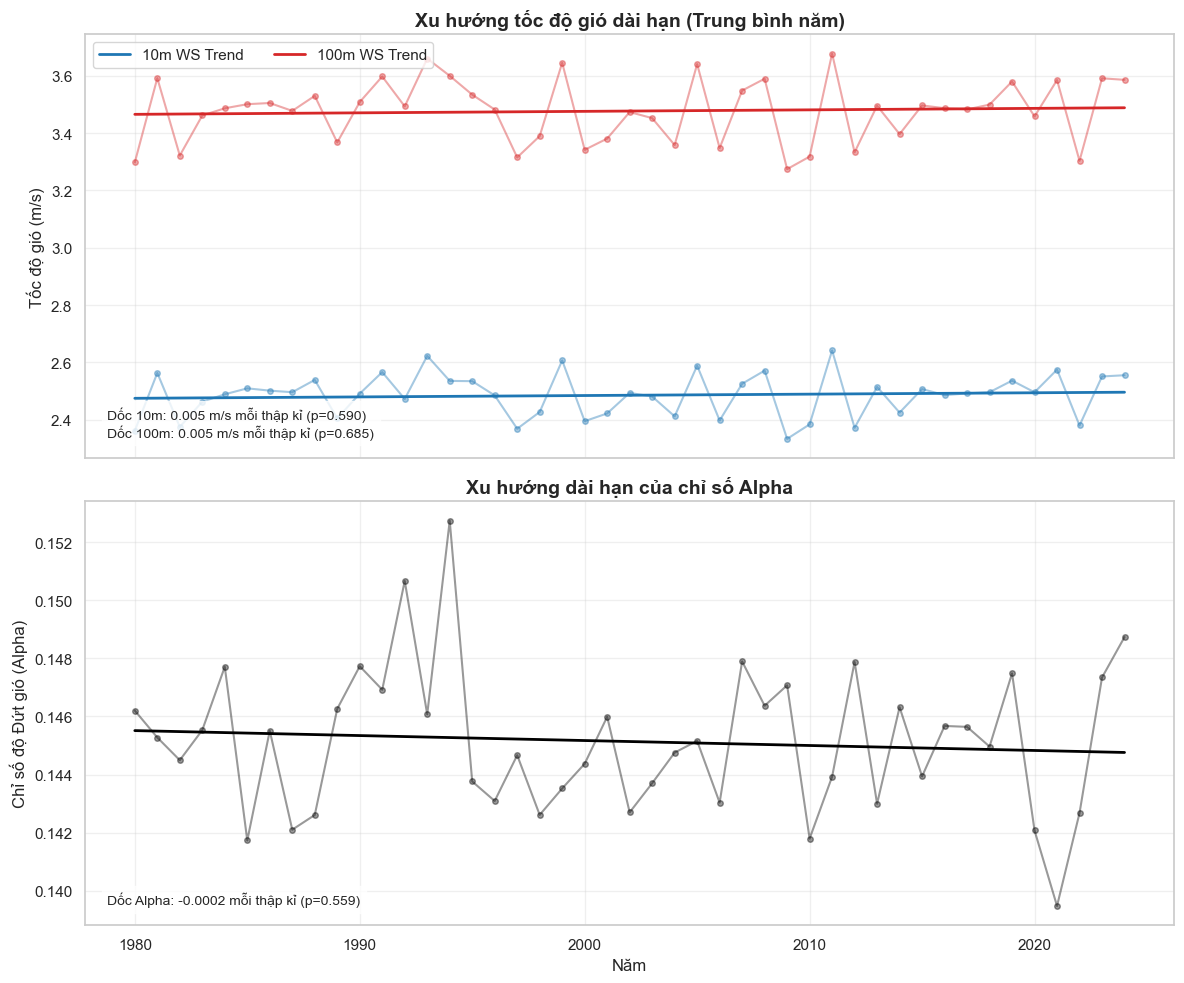
\includegraphics[width=\textwidth]{images/3.14.3.png}
        \caption{Xu hướng tốc độ gió dài hạn}
    \end{subfigure}
    \caption{Phân tích đặc trưng chu kỳ mùa và tính ổn định vận tốc gió liên năm}
    \label{fig:wind_speed_overview}
\end{figure}
\FloatBarrier

\subsubsection{Mật độ công suất gió (WPD) và tần suất vận hành}
Tiềm năng năng lượng gió được thể hiện tại \textbf{Hình \ref{fig:wind_power_density}}.

\begin{itemize}
    \item \textbf{Đặc trưng khí hậu (RQ1):} WPD tại 100m cho thấy xu hướng tăng (+0.66 $W/m^2$/thập kỷ). Tần suất gió đạt ngưỡng vận hành (>3 m/s) chiếm trên 55\% số ngày, xác lập miền Trung là khu vực giàu tiềm năng năng lượng tái tạo.
    \item \textbf{Tác nhân khắc nghiệt (RQ2):} Gia tăng WPD báo hiệu các sự kiện gió mạnh cực đoan mang năng lượng tàn phá lớn hơn. Tỉ lệ gió lặng cao (~43\%) mùa chuyển tiếp gây tích tụ nhiệt lượng và ô nhiễm không khí đô thị.
\end{itemize}

\FloatBarrier
\begin{figure}[H]
    \centering
    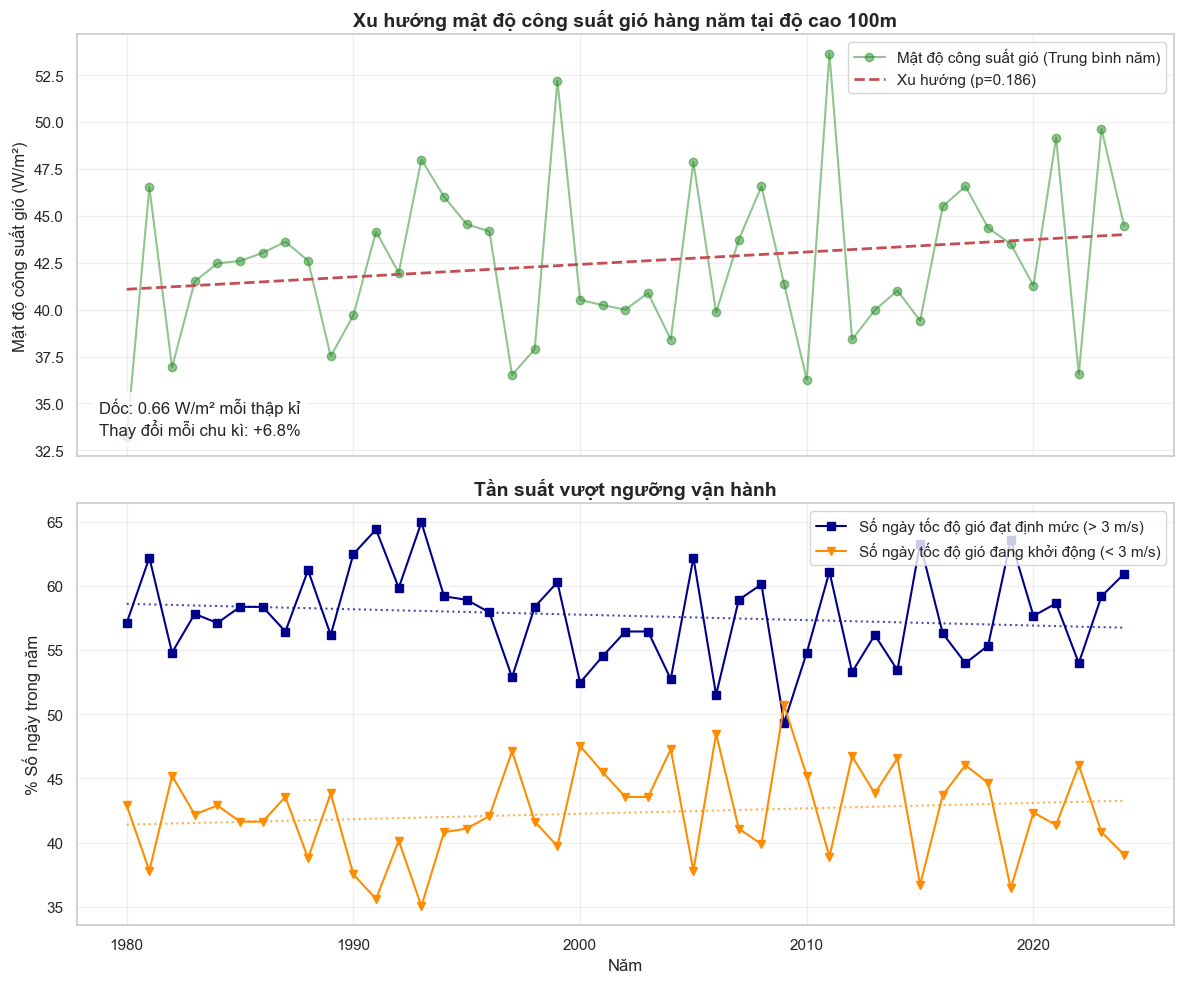
\includegraphics[width=0.7\textwidth]{images/3.14.4.png}
    \caption{Xu hướng mật độ công suất gió (WPD) và tần suất gió theo ngưỡng tại 100m}
    \label{fig:wind_power_density}
\end{figure}
\FloatBarrier

\subsubsection{Ma trận dị thường tốc độ gió hàng tháng}
Biến động liên năm được trực quan hóa tại ma trận \textbf{Hình \ref{fig:wind_anomaly_heatmap}}.

\begin{itemize}
    \item \textbf{Đặc trưng khí hậu (RQ1):} Ma trận phản ánh các dị thường đan xen phi tuyến tính, chứng minh trường gió chịu tác động từ các nhiễu động ngắn hạn. Đặc trưng này xác lập tính chất khó dự báo của trường gió.
    \item \textbf{Tác nhân khắc nghiệt (RQ2):} Dị thường dương mạnh vào cuối năm pha \textbf{La Niña} phản ánh gió mùa Đông Bắc hoạt động dồn dập. Giai đoạn gió yếu gắn liền với \textbf{El Niño}, làm suy giảm khả năng tự làm mát vùng ven biển.
\end{itemize}

\FloatBarrier
\begin{figure}[H]
    \centering
    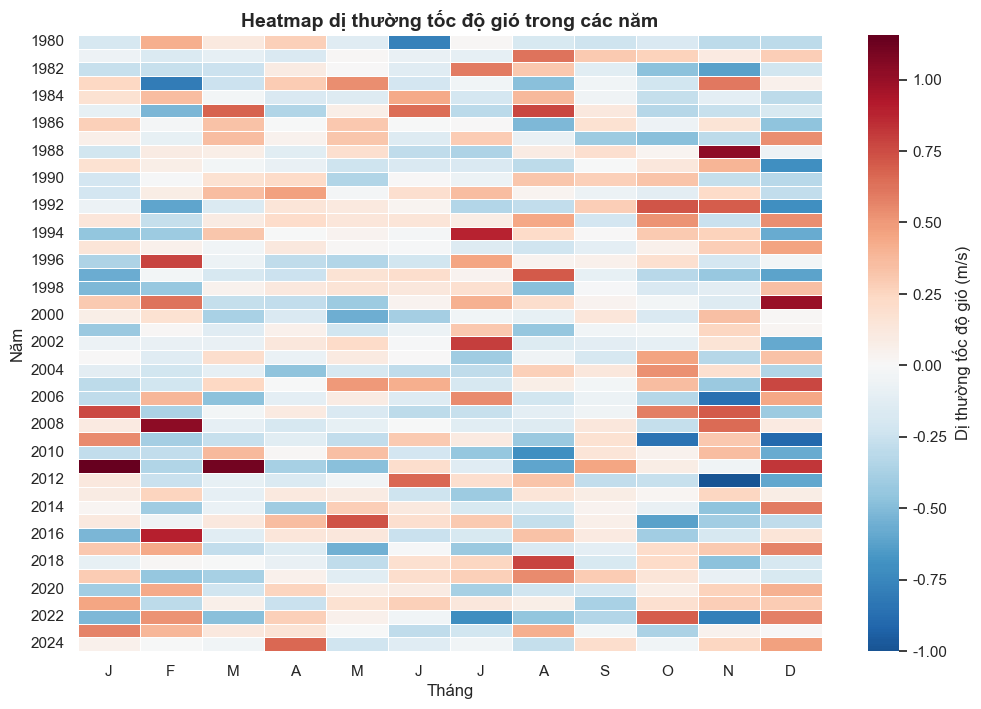
\includegraphics[width=0.85\textwidth]{images/3.14.5.png}
    \caption{Ma trận dị thường tốc độ gió hàng tháng tại miền Trung (1980--2024)}
    \label{fig:wind_anomaly_heatmap}
\end{figure}
\FloatBarrier

\subsubsection{Độ nhất quán của gió mùa Tây Nam \& Sự dịch chuyển phân phối Weibull}
Độ bền bỉ tại \textbf{Hình \ref{fig:wind_const_weibull}(a)} và mật độ tại \textbf{Hình \ref{fig:wind_const_weibull}(b)}.

\begin{itemize}
    \item \textbf{Đặc trưng khí hậu (RQ1):} Gió Tây Nam mùa hạ có độ nhất quán cực cao (~90\%). Phân phối Weibull duy trì cấu trúc ổn định nhưng ghi nhận sự tịnh tiến nhẹ của đỉnh xác suất sang phía vận tốc cao hơn.
    \item \textbf{Tác nhân khắc nghiệt (RQ2):} Chính độ nhất quán của gió Tây Nam duy trì \textbf{hiệu ứng phơn} kéo dài, biến miền Trung thành lõi khô hạn. Việc nới rộng "đuôi" hàm Weibull báo hiệu gia tăng các xung gió giật nguy hiểm trong bão.
\end{itemize}

\FloatBarrier
\begin{figure}[H]
    \centering
    \begin{subfigure}[b]{0.48\textwidth}
        \centering
        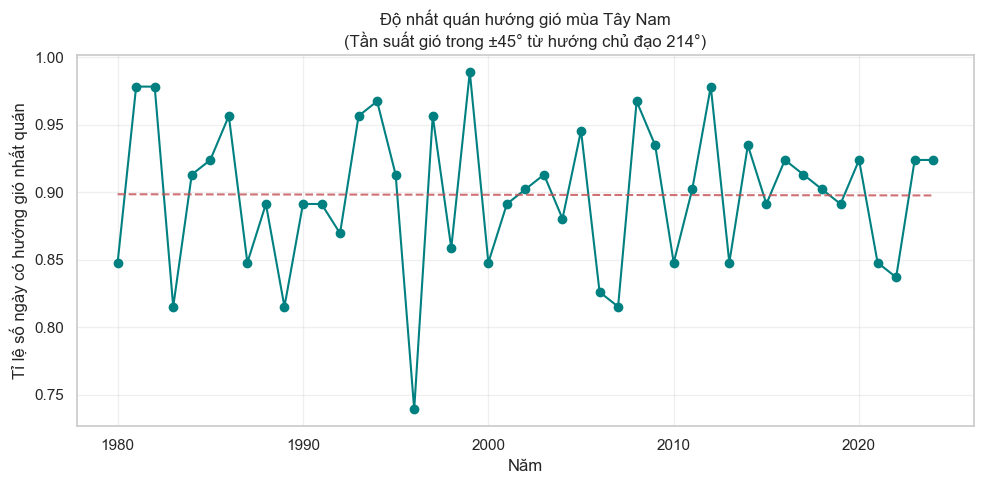
\includegraphics[width=\textwidth]{images/3.14.6.png}
        \caption{Độ nhất quán gió Tây Nam}
    \end{subfigure}
    \hfill
    \begin{subfigure}[b]{0.48\textwidth}
        \centering
        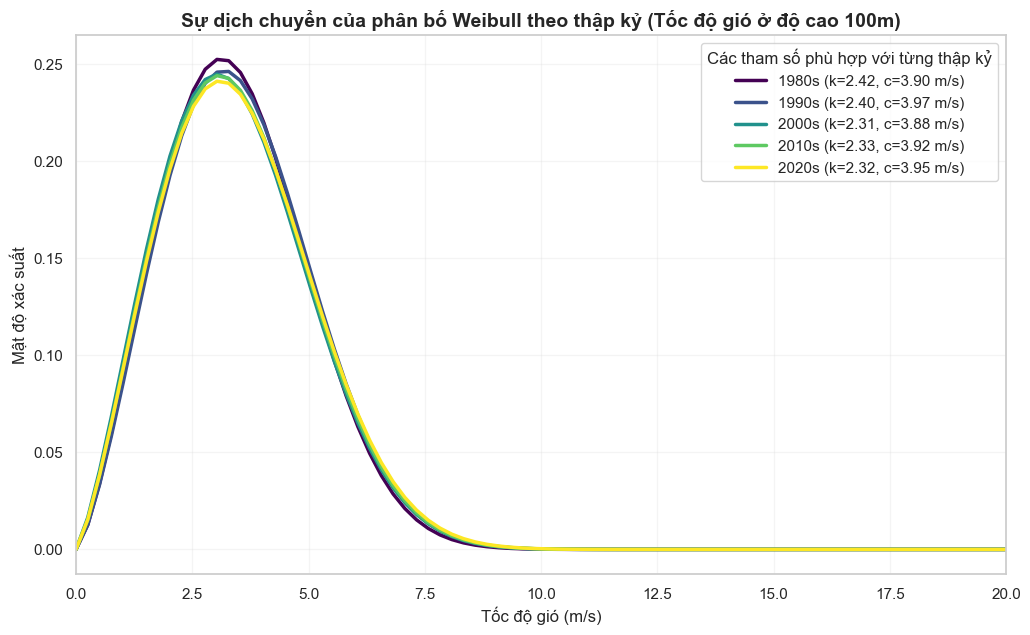
\includegraphics[width=\textwidth]{images/3.14.8.png}
        \caption{Hàm phân phối Weibull}
    \end{subfigure}
    \caption{Phân tích độ bền bỉ luồng gió mùa hạ và dịch chuyển mật độ xác suất vận tốc gió}
    \label{fig:wind_const_weibull}
\end{figure}
\FloatBarrier

\subsubsection{Động lực đứt gãy gió theo mùa và cực đoan}
Chỉ số Alpha tại \textbf{Hình \ref{fig:wind_shear}} thể hiện phân tầng không khí.

\begin{itemize}
    \item \textbf{Đặc trưng khí hậu (RQ1):} Chỉ số Alpha đạt cực đại mùa hè (~0.16), phân tầng gió giữa bề mặt và tầng cao mạnh nhất khi nắng nóng. Đặc trưng này hạn chế sự xáo trộn nhiệt ẩm trong mùa khô.
    \item \textbf{Tác nhân khắc nghiệt (RQ2):} Đỉnh Alpha mùa hè phản ánh thống trị của \textbf{áp thấp nóng phía Tây}, ngăn cản đối lưu lên cao, giam hãm nhiệt lượng sát bề mặt đệm đô thị.
\end{itemize}

\FloatBarrier
\begin{figure}[H]
    \centering
    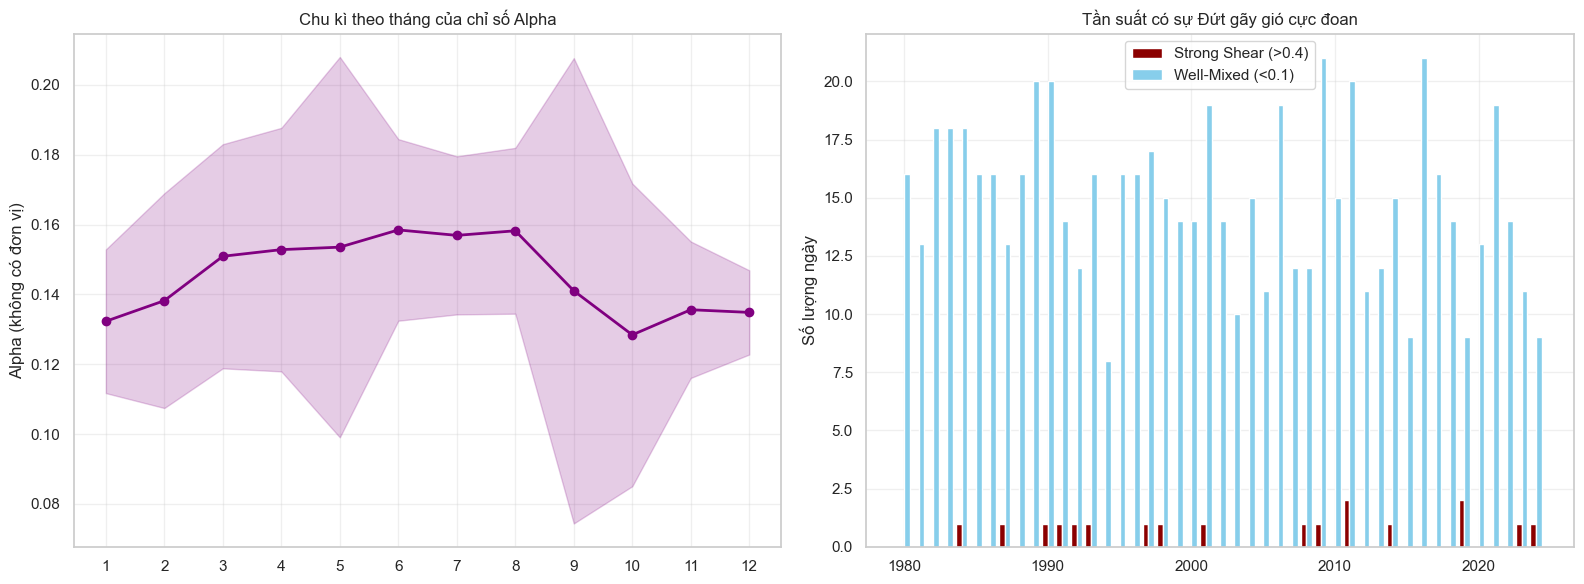
\includegraphics[width=0.7\textwidth]{images/3.14.7.png}
    \caption{Chu kỳ theo tháng của chỉ số Alpha và tần suất đứt gãy gió cực đoan}
    \label{fig:wind_shear}
\end{figure}
\FloatBarrier

\subsection{Phân kỳ ẩm}

\subsubsection{Ma trận dị thường độ hội tụ ẩm hàng tháng}
Tính chất "bồn trũng" được thể hiện qua ma trận tại \textbf{Hình \ref{fig:moisture_anomaly_heatmap}}.

\begin{itemize}
    \item \textbf{Đặc trưng khí hậu (RQ1):} Miền Trung là vùng hội tụ ẩm ròng lớn nhất với các dị thường dương tập trung vào tháng 9--11. Chu kỳ "hút ẩm" từ đại dương chi phối hoàn toàn chế độ mưa bão và lũ lụt.
    \item \textbf{Tác nhân khắc nghiệt (RQ2):} Hội tụ ẩm cực mạnh (tháng 10/2020) là dấu ấn của \textbf{tổ hợp thiên tai} bão và không khí lạnh. Luồng ẩm khi va đập vào \textbf{dãy Trường Sơn} bị cưỡng bức hội tụ, gây đại hồng thủy.
\end{itemize}

\FloatBarrier
\begin{figure}[H]
    \centering
    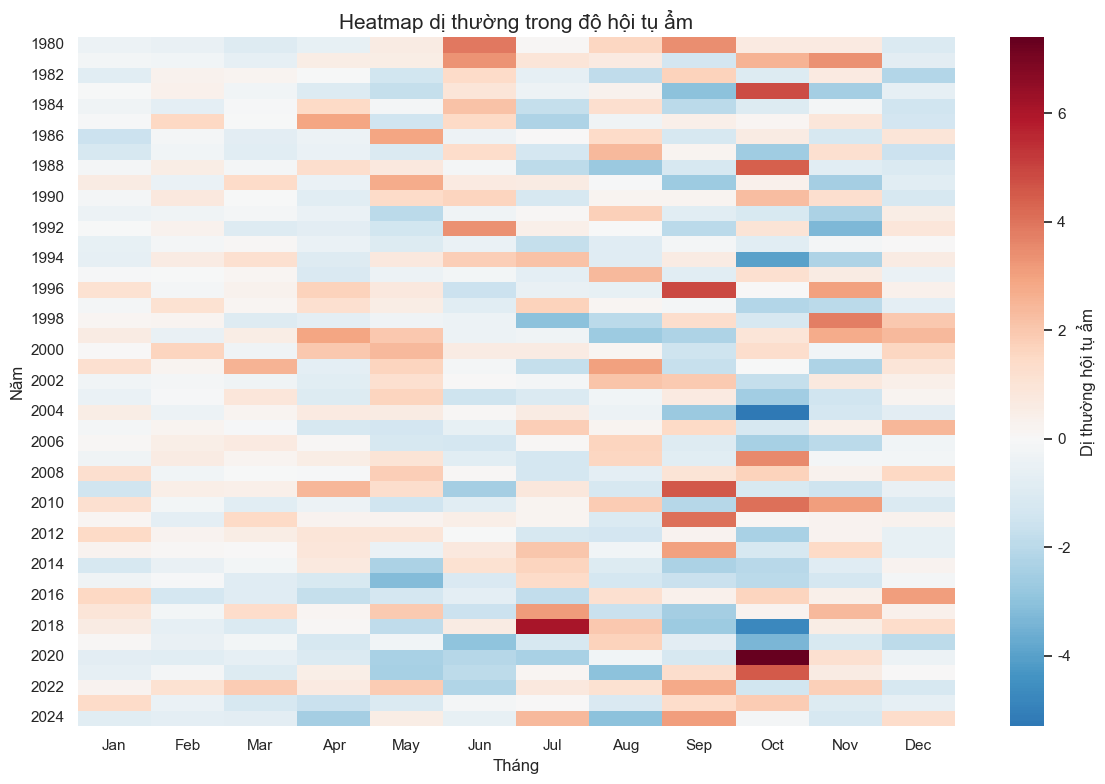
\includegraphics[width=0.85\textwidth]{images/3.15.1.png}
    \caption{Ma trận dị thường độ hội tụ ẩm hàng tháng (1980--2024)}
    \label{fig:moisture_anomaly_heatmap}
\end{figure}
\FloatBarrier

\subsubsection{Xu hướng dài hạn của hội tụ ẩm trung bình năm}
Biến động động lực dài hạn được trình bày tại \textbf{Hình \ref{fig:moisture_conv_trend}}.

\begin{itemize}
    \item \textbf{Đặc trưng khí hậu (RQ1):} Hội tụ ẩm năm duy trì giá trị dương với biên độ biến động lớn. Đặc trưng này khẳng định miền Trung nhận ẩm ròng bền bỉ nhưng cực kỳ nhạy cảm trước biến động khí hậu.
    \item \textbf{Tác nhân khắc nghiệt (RQ2):} Sự xuất hiện dày đặc các điểm cực trị hội tụ ẩm cho thấy các đợt vận chuyển hơi nước đang trở nên \textbf{đột ngột và mãnh liệt hơn}, dẫn đến mưa lũ quét thảm khốc.
\end{itemize}

\FloatBarrier
\begin{figure}[H]
    \centering
    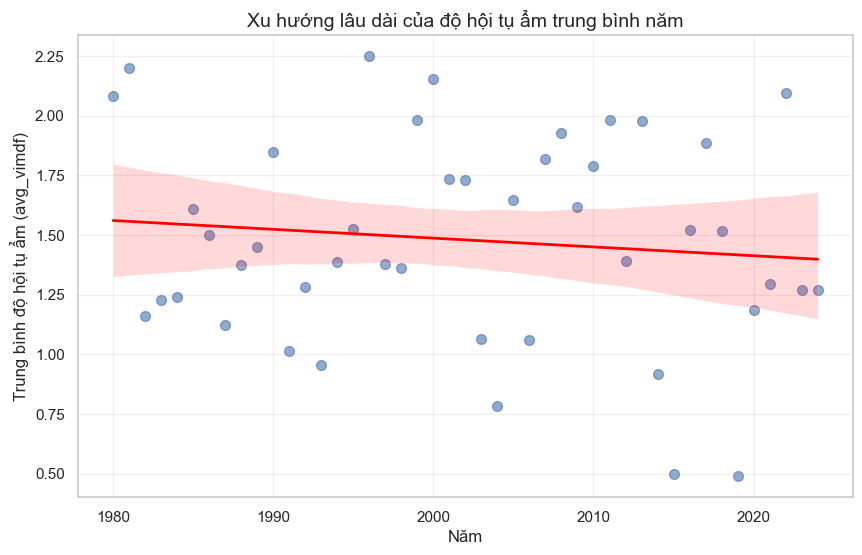
\includegraphics[width=0.7\textwidth]{images/3.15.2.png}
    \caption{Xu hướng biến đổi dài hạn của độ hội tụ ẩm trung bình năm}
    \label{fig:moisture_conv_trend}
\end{figure}
\FloatBarrier

\subsection{Nhiệt độ biển và độ cao sóng}

\subsubsection{Biến động hải văn theo mùa \& Xu hướng nóng lên của biển}
Chu kỳ hải văn tại \textbf{Hình \ref{fig:ocean_general}(a)} và xu hướng tại \textbf{Hình \ref{fig:ocean_general}(b)}.

\begin{itemize}
    \item \textbf{Đặc trưng khí hậu (RQ1):} SST đạt đỉnh tháng 8 (~29.4$^\circ$C), sóng đạt đỉnh mùa đông (>1.5m). SST ven bờ tăng với tốc độ \textbf{+0.179$^\circ$C/thập kỷ}, đồng bộ với xu hướng nóng lên toàn cầu.
    \item \textbf{Tác nhân khắc nghiệt (RQ2):} Biển nóng lên liên tục là tác nhân "tiếp củi" năng lượng cho \textbf{xoáy thuận nhiệt đới}. SST cao khiến bão khi tiến sát bờ có xu hướng duy trì hoặc tăng cấp đột ngột.
\end{itemize}

\FloatBarrier
\begin{figure}[H]
    \centering
    \begin{subfigure}[b]{0.48\textwidth}
        \centering
        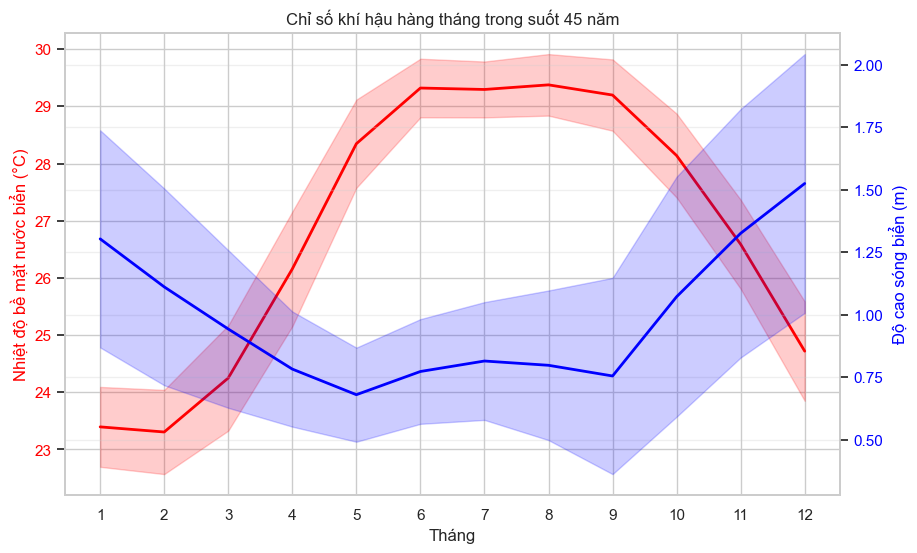
\includegraphics[width=\textwidth]{images/3.16.1.png}
        \caption{Chu kỳ SST và Độ cao sóng}
    \end{subfigure}
    \hfill
    \begin{subfigure}[b]{0.48\textwidth}
        \centering
        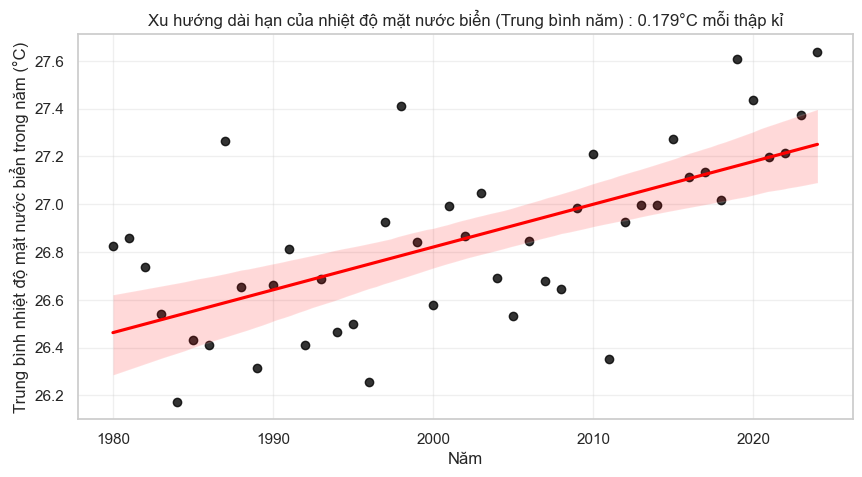
\includegraphics[width=\textwidth]{images/3.16.2.png}
        \caption{Xu hướng dài hạn SST}
    \end{subfigure}
    \caption{Đặc trưng trạng thái nhiệt - động lực mặt nước biển ven bờ miền Trung}
    \label{fig:ocean_general}
\end{figure}
\FloatBarrier

\subsubsection{Ma trận dị thường nhiệt độ mặt nước biển (SST)}
Biến động SST lịch sử được trực quan hóa qua ma trận tại \textbf{Hình \ref{fig:sst_anomaly_heatmap}}.

\begin{itemize}
    \item \textbf{Đặc trưng khí hậu (RQ1):} Ma trận SST lật trạng thái sang "nóng" tuyệt đối sau mốc 2014. Đặc trưng này phản ánh sự thay đổi căn bản trong chế độ nhiệt của vùng biển ven bờ trong thập kỷ qua.
    \item \textbf{Tác nhân khắc nghiệt (RQ2):} Nền nhiệt biển cao bất thường tập trung vào \textbf{El Niño} phá hủy hệ sinh thái và làm đảo lộn quy luật bão. Tác nhân này khiến các hệ thống thời tiết trên Biển Đông trở nên dị thường.
\end{itemize}

\FloatBarrier
\begin{figure}[H]
    \centering
    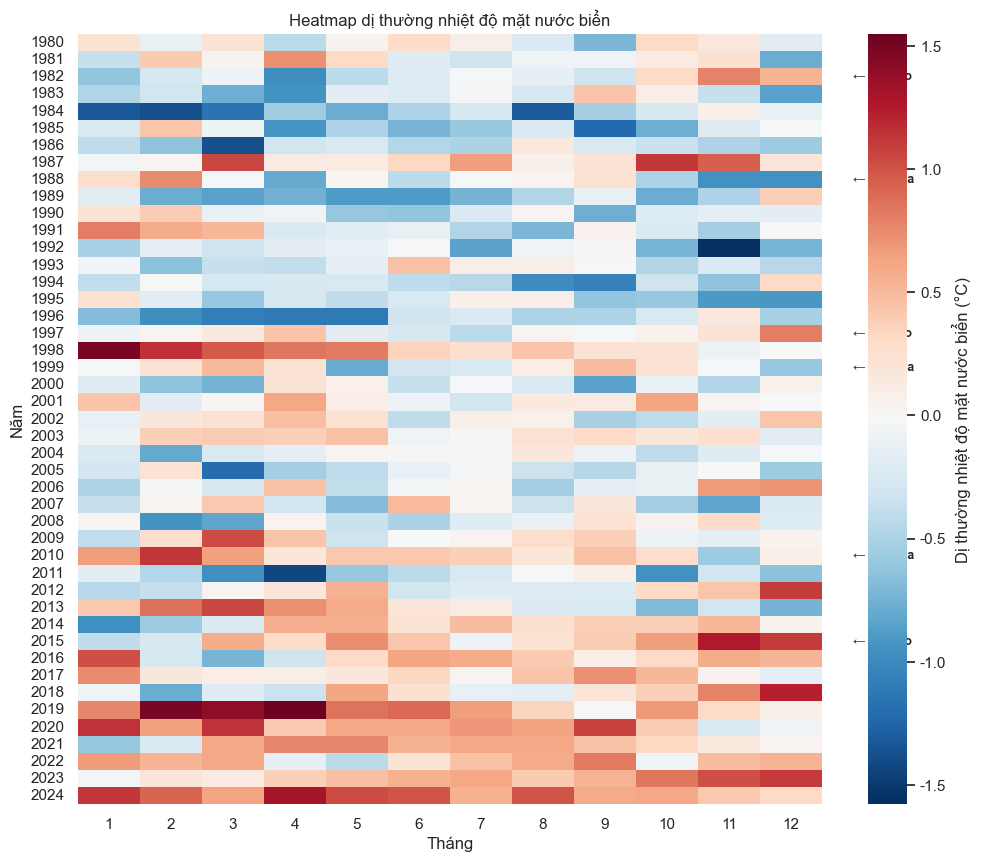
\includegraphics[width=0.85\textwidth]{images/3.16.3.png}
    \caption{Ma trận dị thường nhiệt độ mặt nước biển (SST) hàng tháng (1980--2024)}
    \label{fig:sst_anomaly_heatmap}
\end{figure}
\FloatBarrier

\subsubsection{Sóng nhiệt đại dương (MHW) \& Tần suất sóng cực đoan}
Cực đoan hải văn tại \textbf{Hình \ref{fig:ocean_extreme}(a)} và trường sóng tại \textbf{Hình \ref{fig:ocean_extreme}(b)}.

\begin{itemize}
    \item \textbf{Đặc trưng khí hậu (RQ1):} Số ngày MHW bùng nổ lên ngưỡng 100--160 ngày/năm. Tần suất sóng cực đoan phản ánh tính nhạy bén của trường sóng trước biến động động lực khí quyển.
    \item \textbf{Tác nhân khắc nghiệt (RQ2):} Sự bùng nổ MHW năm 2024 minh chứng tác động cộng hưởng giữa biến đổi khí hậu và El Niño. Các đỉnh sóng cực đoan gắn liền với \textbf{bão mạnh và gió mùa Đông Bắc}, uy hiếp an toàn đê kè.
\end{itemize}

\FloatBarrier
\begin{figure}[H]
    \centering
    \begin{subfigure}[b]{0.48\textwidth}
        \centering
        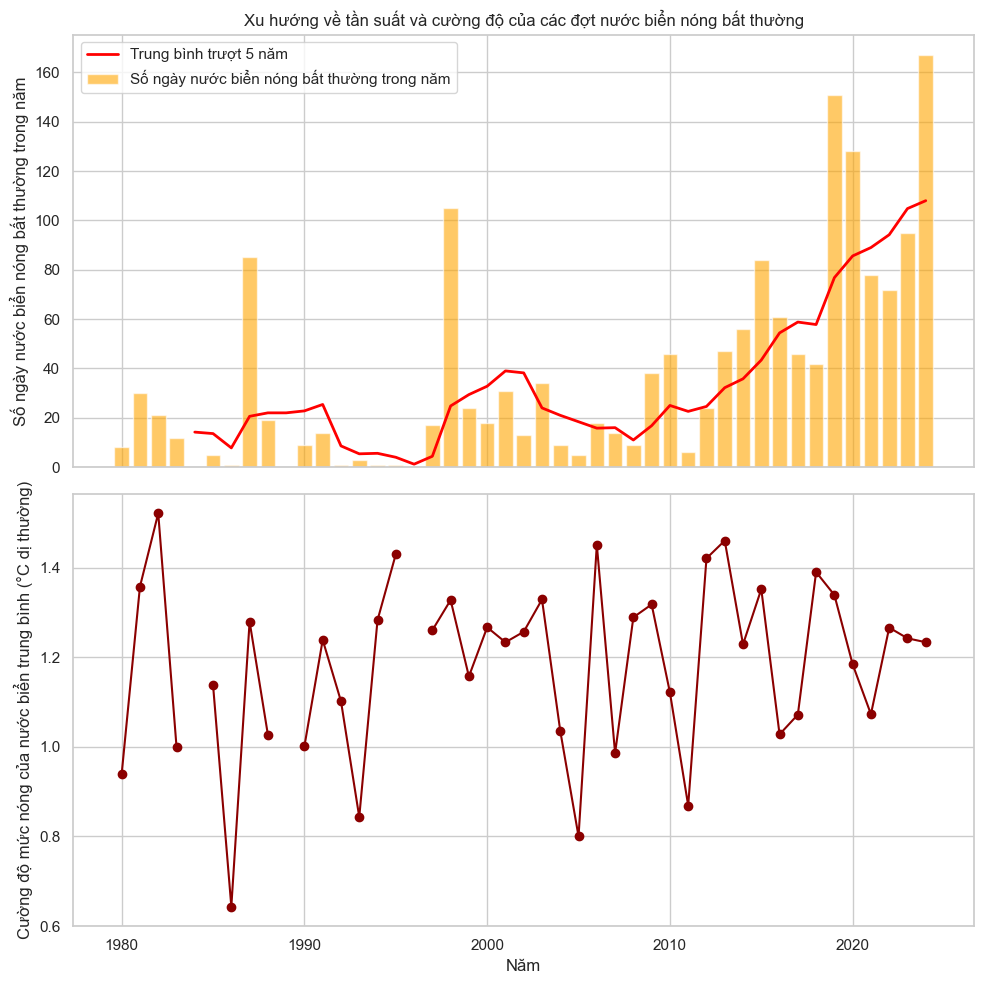
\includegraphics[width=\textwidth]{images/3.16.4.png}
        \caption{Sóng nhiệt đại dương MHW}
    \end{subfigure}
    \hfill
    \begin{subfigure}[b]{0.48\textwidth}
        \centering
        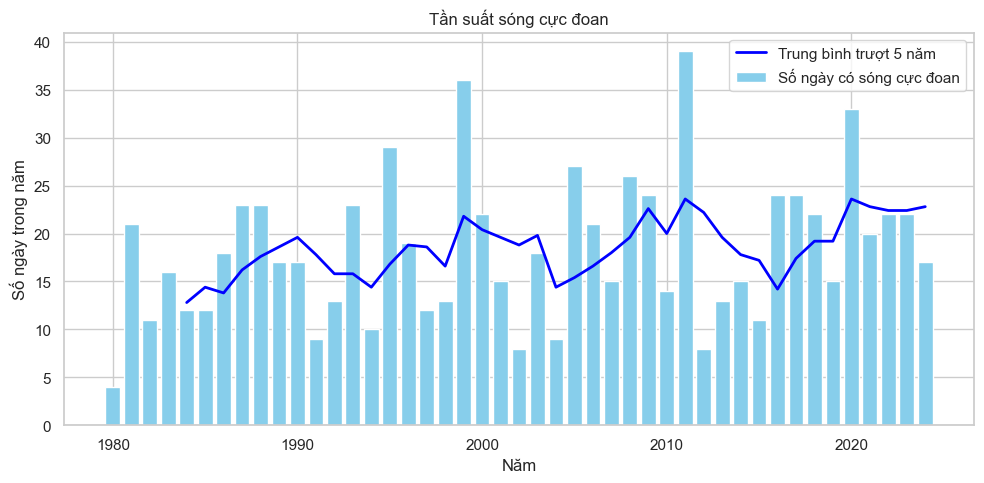
\includegraphics[width=\textwidth]{images/3.16.5.png}
        \caption{Tần suất sóng cực đoan}
    \end{subfigure}
    \caption{Phân tích cực đoan nhiệt đại dương và động lực trường sóng ven bờ}
    \label{fig:ocean_extreme}
\end{figure}
\FloatBarrier

% =========================================================================
% SECTION 4 VÀ 5: PHẦN KẾT LUẬN (ẢNH SẼ BỊ CHẶN LẠI KHÔNG THỂ NHẢY XUỐNG ĐÂY)
% =========================================================================
\FloatBarrier
\section{Kết luận}

Thông qua quá trình phân tích toàn diện các yếu tố khí hậu của khu vực miền Trung Việt Nam, báo cáo đã làm rõ được bức tranh khí hậu đặc thù và phức tạp của vùng đất này. Từ các yếu tố cơ bản như nhiệt độ không khí và bề mặt, nhiệt độ đất, điểm sương và độ ẩm, cho đến các yếu tố động lực như chế độ gió, phân kỳ ẩm, bất ổn định đối lưu, tất cả đều được xem xét và đánh giá một cách hệ thống. Kết quả cho thấy miền Trung là khu vực có sự phân hóa khí hậu rõ rệt cả theo không gian lẫn thời gian, với sự tương tác phức tạp giữa địa hình Trường Sơn, Biển Đông và các hệ thống thời tiết nhiệt đới là nguyên nhân cốt lõi tạo nên đặc trưng khí hậu độc đáo của vùng.

Về các yếu tố nhiệt và ẩm, phân tích đã chỉ ra sự phân hóa rõ ràng giữa sườn Đông và sườn Tây Trường Sơn trong chế độ nhiệt độ và lượng mưa. Hiệu ứng phơn tạo nên mùa khô gay gắt trong khi nguồn ẩm từ Biển Đông lại tập trung gây mưa lớn trong thời gian ngắn, dẫn đến sự đối lập cực đoan giữa hai mùa. Các yếu tố liên quan đến chu trình nước như lượng mưa, bốc hơi, độ ẩm đất và dòng chảy cũng cho thấy mối quan hệ tương tác chặt chẽ, phản ánh một hệ thống thủy văn khí hậu vận hành theo quy luật riêng biệt so với các khu vực khác trong cả nước. Bức xạ mặt trời và thông lượng nhiệt bề mặt đóng vai trò quan trọng trong việc điều tiết nhiệt độ và bốc hơi, đặc biệt trong các tháng mùa khô khi lượng mây che phủ thấp.

Về phía các yếu tố động lực và cấu trúc khí quyển, chế độ gió và phân kỳ ẩm đã làm rõ cơ chế vận chuyển hơi nước vào khu vực, trong khi bất ổn định đối lưu giải thích cho sự hình thành của các hình thái mưa cực đoan đặc trưng. Độ che phủ mây và lượng hơi nước cột khí quyển cũng cho thấy sự biến động theo mùa rõ rệt, phù hợp với chu kỳ hoạt động của gió mùa. Nhiệt độ biển và độ cao sóng tại vùng ven bờ Biển Đông cũng được ghi nhận là có mối liên hệ mật thiết với cường độ và hướng di chuyển của các hệ thống thời tiết ảnh hưởng đến khu vực.

Nhìn chung, các kết quả phân tích trong báo cáo này góp phần cung cấp một cơ sở khoa học có hệ thống về đặc trưng khí hậu miền Trung Việt Nam. Thông qua việc xây dựng notebook phân tích và dashboard trực quan hóa, nhóm mong muốn không chỉ phục vụ mục đích học thuật mà còn giúp người xem không chuyên có thể dễ dàng nắm bắt được thực trạng khí hậu của khu vực. Trong tương lai, hướng nghiên cứu có thể được mở rộng theo chiều sâu bằng cách tích hợp thêm dữ liệu chuỗi thời gian dài hạn để phân tích xu hướng biến đổi, hoặc mở rộng phạm vi so sánh với các khu vực khác trong cả nước nhằm làm nổi bật hơn nữa tính đặc thù của khí hậu miền Trung trong bối cảnh biến đổi khí hậu toàn cầu.

\section{Tài liệu tham khảo}
\begin{enumerate}
    \item Hersbach, H., Bell, B., Berrisford, P., Hirahara, S., Horányi, A., Muñoz‐Sabater, J., ... \& Thépaut, J. N. (2020). The ERA5 global reanalysis. \textit{Quarterly Journal of the Royal Meteorological Society}, 146(730), 1999-2049.
    
    \item Muñoz-Sabater, J., Dutra, E., Agustí-Panareda, A., Albergel, C., Arduini, G., Balsamo, G., ... \& Thépaut, J. N. (2021). ERA5-Land: A state-of-the-art global land surface reanalysis dataset. \textit{Earth System Science Data}, 13(9), 4349-4383.
    
    \item Nguyễn Đức Ngữ, \& Nguyễn Trọng Hiệu (2004). \textit{Khí hậu và tài nguyên khí hậu Việt Nam}. Nhà xuất bản Nông nghiệp, Hà Nội.
    
    \item Trần Thục, Nguyễn Văn Thắng, Huỳnh Thị Lan Hương, Nguyễn Đăng Mậu, Trường Bá Nghiêm, \& Nguyễn Xuân Hiển (2016). \textit{Kịch bản biến đổi khí hậu và nước biển dâng cho Việt Nam}. Nhà xuất bản Tài nguyên - Môi trường và Bản đồ Việt Nam.
    
    \item Phan Văn Tân, \& Ngô Chí Tuấn (2014). Biến đổi khí hậu ở miền Trung Việt Nam: Xu hướng quá khứ và kịch bản tương lai. \textit{Tạp chí Khoa học ĐHQGHN: Các Khoa học Trái đất và Môi trường}, 30(2), 1-13.
    
    \item Nguyễn Minh Trường, Phan Văn Tân, \& Tập thể tác giả (2019). Đánh giá chất lượng dữ liệu lượng mưa tái phân tích ERA5 trên khu vực Trung Bộ, Việt Nam. \textit{Tạp chí Khoa học Tài nguyên và Môi trường}, (28), 45-56.
    
    \item Vũ Thanh Hằng, Phan Văn Tân, \& Ngô Thị Thanh Hương (2012). Thống kê các đặc trưng nắng nóng và cực đoan nhiệt độ ở Việt Nam giai đoạn 1961-2010. \textit{Tạp chí Khí tượng Thủy văn}, (617), 33-39.
    
    \item Bowen, I. S. (1926). The ratio of heat losses by conduction and by evaporation from any water surface. \textit{Physical Review}, 27(6), 779-787.
    
    \item Trenberth, K. E., Fasullo, J. T., \& Kiehl, J. (2009). Earth's global energy budget. \textit{Bulletin of the American Meteorological Society}, 90(3), 311-324.
    
    \item Monahan, A. H. (2006). The probability distribution of sea surface wind speeds. \textit{Journal of Climate}, 19(19), 4978-4992.
    
    \item Riemann-Campe, K., Fraedrich, K., \& Lunkeit, F. (2009). Global climatology of Convective Available Potential Energy (CAPE) in ECMWF reanalysis data. \textit{International Journal of Climatology}, 29(8), 1141-1151.
    
    \item Allan, R. P., \& Soden, B. J. (2008). Atmospheric warming and the amplification of precipitation extremes. \textit{Science}, 321(5895), 1481-1484.

    \item Vicente-Serrano, S. M., Beguería, S., \& López-Moreno, J. I. (2010). A multiscalar drought index sensitive to global warming: the standardized precipitation evapotranspiration index. \textit{Journal of Climate}, 23(7), 1696-1718.
    
    \item Sheffield, J., Goteti, G., \& Wood, E. F. (2006). Development of a 50-year high-resolution global dataset of meteorological forcings for land surface modeling. \textit{Journal of Climate}, 19(13), 3088-3111.
    
    \item Bộ Tài nguyên và Môi trường (2021). \textit{Báo cáo kịch bản biến đổi khí hậu cập nhật cho khu vực Trung Bộ và xu thế thiên tai hệ thống}. Tổng cục Khí tượng Thủy văn Việt Nam.
\end{enumerate}

\end{document}